\chapter{Four Formulations of the SEAS Problem}

\section{First Order Differential Equation}
The problem stated in \autoref{ssec:physicalDescriptionSEAS2D} is a first order DAE, as the involving terms only depend on the unknown quantities and at most there first time derivatives:
\begin{align}
    \dot{S_i} &= V_i \label{eq:SEASDAE_dV_dt} \\
	\dot{\psi_i} &= g(\psi_i, V_i) =\frac{bV_0}{L}\left(e^{\frac{f_0-\psi_i}{b}} - \frac{V_i}{V_0}\right) \label{eq:SEAS_DAE_ageing_law} \\
	0 &= f_i(U,S,\psi,V) = \tau_i(U,S) - a\sigma_n\text{arsinh}\left(\frac{V_i}{2V_0}e^{\frac{\psi_i}{a}}\right) -\eta V_i \label{eq:SEASDAE_frictionLaw}\\
    0 &= AU - b(S) \label{eq:SEAS_DAE_AU=b}  
\end{align}
The index $i\in[0,n]$ refers to all interpolation points of the elements located on the fault, meaning that $S_i$, $V_i$ and $\psi_i$ are respectively the slip, the velocity and the value of the state variable on the fault. The matrix-vector system in \autoref{eq:SEAS_DAE_AU=b} stems from the DG formulation of the Poisson problem and needs to be solved for all nodes with index $j\in[0,N]$ in the DG domain. Usually, there are much more nodes in the full domain then purely on the fault, so $n \ll N$. The slip $S_i$ at the fault is related to the displacement $U_j$ by $\llbracket U_j \rrbracket = U_j^+ - U_j^- = -S_i$, where $j$ is the index of the fault node $i$ in the discretization of the full DG domain. The displacements $U_j^+$ and $U_j^-$ correspond to the displacements on the two sides of the fault, for the current symmetric problem, they have the same magnitude with opposite signs. Outside of the fault, the term $S$ is used to enforce boundary conditions on the domain, and typically increases with time, simulating constant tectonic movements of the plates. Nodes on the fault will first resist to this environment slip and when the forces reach a certain level, an earthquake is triggered. \\
To use implicit time solvers, a nonlinear equation has to be solved at each time step. For this purpose, Newton iterations are often used, however they require the Jacobian matrices of the right-hand side functions in (\ref{eq:SEAS_DAE_ageing_law}) and (\ref{eq:SEASDAE_dV_dt}). In general, if it is unknown, it is approximated along with the solution during the Newton iteration using for instance a Broyden iteration [cite Broyden]. However, this impairs the convergence speed of the Newton iteration compared to the analytical expression. It is especially relevant if a DAE formulation of the problem is chosen, for which an iterative solver is indispensable. An analytic expression of the Jacobian is provided for both the ODE and the DAE formulations of the problem, so that the Newton iterations can be solved efficiently when using implicit methods.
 

\subsection{Formulation as a first order ODE}
\subsubsection{Problem}
The first approach to solve the problem is to formulate the system as a classical ODE. The solution vector contains the values for the slip and for the state variable, and at each timestep, the the slip rate $V$ is calculated from \autoref{eq:SEASDAE_frictionLaw} from the state with an iterative solver.
\begin{align}
	\label{eq:ODE_formulation_SEAS}
	x &= \begin{pmatrix}
		S \\ \psi
	\end{pmatrix} & \dot{x} &= \begin{pmatrix}
								  \dot{S} \\ \dot{\psi}
							   \end{pmatrix} = \begin{pmatrix}
												   V(S,\psi) \\ g(\psi, V)
											   \end{pmatrix} = F
\end{align} 
Such a formulation allows us to use many well-known and proved numerical schemes, both implicit and explicit. 

\subsubsection{Jacobian matrix}
\label{sssec:Jacobian_ODE}
For the ODE formulation in \autoref{eq:ODE_formulation_SEAS}, it is not straightforward to calculate the Jacobian matrix because of the implicit evaluation of the slip rate within the right-hand side function. The matrix $\mathbf{J}_{\psi,S}(F)$ consists of four block matrices, which each contains the Jacobians related to the two quantities:
\begin{equation}
\label{eq:Jacobian_ODE_formulation}
\mathbf{J}_{\psi_j,S_j}\left(F_i\left(\psi,V(\psi,S)\right)\right) = \begin{pmatrix} 
\frac{\partial V_i}{\partial S_j} &
\frac{\partial V_i}{\partial \psi_j} \\ 
\frac{\partial g(\psi_i,V_i)}{\partial S_j} &
\frac{\partial g(\psi_i,V_i)}{\partial \psi_j}  \end{pmatrix}
\end{equation}
In a first step, the partial derivatives of the slip rate $V$ will be calculated. As this quantity is obtained implicitly from the friction law in \autoref{eq:SEASDAE_frictionLaw}, the implicit function theorem has to be applied. The function $f()$ is continuously differentiable and its Jacobian matrix with respect to the slip rate $\frac{\partial f}{\partial V}$ is invertible. Indeed, from the analytic expression in \autoref{eq:partial_df_dV}, it appears that the matrix is diagonal and its entries are all non-zero. All necessary conditions to apply the implicit function are fulfilled and it states that the partial derivatives of $V$ are given by the product:
\begin{align}
\frac{\partial V}{\partial S} &= -\left(\frac{\partial f}{\partial V}\right)^{-1}\frac{\partial f}{\partial S} \\ 
\frac{\partial V}{\partial \psi} &= -\left(\frac{\partial f}{\partial V}\right)^{-1}\frac{\partial f}{\partial \psi} 
\end{align}
Two of the occurring Jacobian matrices can be easily obtained from the respective derivatives of the friction law. 
\begin{equation}
\frac{\partial f_i(S,\psi,V)}{\partial \psi_j} = \left( -\frac{\sigma_n}{2V_0} \frac{Ve^{\frac{\psi_i}{a}}}{\sqrt{\frac{e^{\frac{2\psi_i}{a}}V_i^2}{4V_0^2}+1}}\right)\delta_{ij} 
\label{eq:partial_df_dpsi}
\end{equation}	
\begin{equation}
\frac{\partial f_i(S,\psi,V)}{\partial V_j} = \left( -\frac{\sigma_na}{2V_0} \frac{e^{\frac{\psi_i}{a}}}{\sqrt{\frac{e^{\frac{2\psi_i}{a}}V_i^2}{4V_0^2}+1}}-\eta\right)\delta_{ij} 
\label{eq:partial_df_dV}
\end{equation}
Since $\frac{\partial f}{\partial V}$ is a diagonal matrix, its inverse is very easy to calculate and does not require to solve a linear system of equations. The evaluation of the last missing partial derivative is more complex to obtain and will be one reason for a partial filling of the Jacobian matrix.
\begin{align}
\label{eq:partialDerivative_df_dS}
\frac{\partial f_i}{\partial S_j} = \frac{d \tau_i(U)}{d S_j} = \frac{\partial \tau_i(U)}{\partial U_k}\frac{\partial U_k}{\partial S_j} + \frac{\partial \tau_i(U)}{\partial S_j}
\end{align}
The problem shifted to calculate the partial derivative $\frac{\partial U}{\partial S}$. Since $U = A^{-1}b(S)$ and the matrix $A$ does not depend on $S$, we just need to find the derivative of $b(S)$. We get, for elements on the fault:
\begin{align}
\frac{\partial b_i(S)}{\partial S_j} &= \frac{\partial }{\partial S_j}\int_e \eta \{\{c_{mnkl}\epsilon_{kl}(w)\eta_n^e\}\}\llbracket U_m \rrbracket + \frac{\delta_e}{|e|^\beta}\llbracket U_m \rrbracket\llbracket w_m \rrbracket dx
\end{align}
As already stated earlier, we have $\llbracket U_i \rrbracket = -S_i$, therefore we can straight eliminate this term. On all other interpolation points not located on the fault, the right hand side $b$ does not depend on the fault displacement $S$ and the derivatives at these points consequently vanish. We then obtain:
\begin{equation}
\frac{\partial b_i(S)}{\partial S_j} = -\int_e 
\eta  \{\{c_{jnkl}\epsilon_{kl}(w)\eta_n^e\}\} +
\frac{\delta_e}{|e|^\beta}\llbracket w_j \rrbracket dx
\end{equation}
This expression can be calculated by plugging the unit vector $e^i$ as argument of the right-hand side vector $b$. The Jacobian term $\frac{\partial U_i}{\partial S_j}$ is therefore evaluated by applying the solver method of the Poisson problem to the unit vectors as slips. We get:
\begin{equation}
\frac{\partial U_i}{\partial S_j} = A_{ik}^{-1}b_k(e^i)
\end{equation}
The traction term $\tau(U,S)$ is calculated as $\tau = \mu \frac{\partial u}{\partial x_i}n_i$, and is numerically approximated on the nodal basis as $\tau_p = M_{rp}^{-1}e_{qr}^Tw_q(\nabla u)_{kq}n_{kq}$, where $M$ is the mass matrix of the fault basis, $e^T$ maps from fault to quadrature points, $w$ are the quadrature weights and $n$ is the normal at the quadrature points. The gradient of $u$ is approximated by $(\nabla u)_{pq} = \frac{1}{2}\left(D_{lpq}^0u_l^0 + D_{lpq}^1u_l^1\right) + c_0\left(E_{lq}^0u_l^0 - E_{lq}^1u_l^1 - f_q\right)n_{pq}$. The tensor $E$ maps from the quadrature points to the element basis and $D$ is its gradient and the superscripts $0$ and $1$ refer to the adjacent elements on opposite sides of the fault. The term $f_q$ denotes the actual slip transformed to the quadrature points. The evaluation of the derivative of the traction with respect to the displacement requires to derivate the gradient of the displacement with respect to itself. We obtain: 
\begin{align}
\frac{(\nabla u)_{pq}}{\partial u_k} &= \frac{1}{2}\left(D_{lpq}^0\frac{\partial u_l^0}{\partial u_k} + D_{lpq}^1\frac{\partial u_l^1}{\partial u_k}\right) + c_0\left(E_{lq}^0\frac{\partial u_l^0}{\partial u_k} - E_{lq}^1\frac{\partial u_l^1}{\partial u_k}\right)n_{pq} \\
&= \frac{1}{2}\left(D_{lpq}^0\delta_{lk}^0 + D_{lpq}^1\delta_{lk}^1\right) + c_0\left(E_{lq}^0\delta_{lk}^0 - E_{lq}^1\delta_{lk}^1\right)n_{pq} \\
&= \frac{1}{2}\left(D_{kpq}^0 + D_{kpq}^1\right) + c_0\left(E_{kq}^0 - E_{kq}^1\right)n_{pq} 
\end{align}
And further we get: 
\begin{equation}
\frac{\partial \tau_p}{\partial u_l} = M_{rp}^{-1}e_{qr}^Tw_q
\frac{(\nabla u)_{kq}}{\partial u_l}n_{kq}
\end{equation}
In addition, the traction needs to be derivated with respect to the current slip directly for the term $\frac{\partial \tau_i(U)}{\partial S_j}$, which is contained in the term $f_q = e_{qj}S_j$. It appears again in the gradient, so its derivative with respect to the slip is also needed. 
\begin{align}
\frac{(\nabla u)_{pq}}{\partial S_j} = -c_0 \frac{\partial f_q}{\partial S_j}n_{pq} 
= -c_0 e^T_{qk}\frac{\partial S_k}{\partial S_j}n_{pq} 
= -c_0 e^T_{qj}n_{pq} \\	
\end{align}
With this expression, we obtain: 
\begin{equation}
\frac{\partial \tau_p}{\partial S_j} = -M_{rp}^{-1}e_{qr}^Tw_qc_0e^T_{qj}n_{kq}n_{kq}
\end{equation}
This derivative term does not depend on the current slip anymore but only on the geometry of the discretization, so it can be calculated once at the beginning of the simulation. All components of the remaining partial derivative in \autoref{eq:partialDerivative_df_dS} are now available and the Jacobian matrices of the slip rate with respect to the slip and to the state variable can be calculated. \\
To express the full Jacobian matrix of the ODE in \autoref{eq:Jacobian_ODE_formulation}, the partial derivatives of the ageing law $g(\psi, V)$ are still missing. They can be expressed in term of the already known partial derivatives: 
\begin{align}
\frac{\partial g_i}{\partial S_j} &= -\frac{b}{L}\frac{\partial V}{\partial S} \\
\frac{\partial g_i}{\partial S_j} &= -\frac{V_0}{L}e^{\frac{f_0 - \psi}{b}}\delta_{ij} -
\frac{b}{L}\frac{\partial V}{\partial \psi}
\end{align}



\subsection{Formulation as a DAE}
\subsubsection{Problem}
The ODE form looks pretty and like an easy-to-tackle numerical problem, but may run into some trouble because of the implicit evaluation of the slip rate, which is treated independently of the numerical integration. Alternatively, the friction law could be solved for the slip rate together with the time-variant solution components. The solution vector is then extended by one quantity, and the evaluation of the slip rate with a separate iterative does not occur anymore.
\begin{align}
	\label{eq:DAE_formulation_SEAS}
	x &= \begin{pmatrix}
			S \\ \psi \\ V
		 \end{pmatrix} & \dot{x} &= \begin{pmatrix}
										\dot{S} \\ \dot{\psi} \\ 0
									\end{pmatrix} = \begin{pmatrix}
										V \\ g(\psi, V) \\ f(S,\psi,V)
									\end{pmatrix}
\end{align}
This system cannot be used anymore with pure explicit solvers, since no time discretization can be set up for the algebraic equation. It is however well-suited for implicit methods, which iteratively solve for the time-variant quantities $S$ and $\psi$ as well for the algebraic state $V$. A notable advantage of this formulation is that the tolerances of the numerical solver can be specified independently for $S$, $\psi$ and $V$, whereas in the ODE formulation of the problem, the error control is limited to the parameters $S$ and $\psi$. \\
The PETSc interface requires us to provide a DAE in the form
\begin{align}
	F(t, x,\dot{x}) = G(t,x) 
\end{align}
where the left-hand side function $F()$ depends on the solution vector and its time derivative whereas the right-hand side function $G()$ only depends on the solution vector. For now, we choose a fully implicit formulation of the problem, in which $G()$ vanishes. The DAE can then be expressed in the following way: 
\begin{align}
\label{eq:DAE_extended_formulation_SEAS}
	x &= \begin{pmatrix}
		S \\ \psi \\ V
	\end{pmatrix} & F(t, x,\dot{x}) &= \begin{pmatrix}
	 	V - \dot{S} \\ g(\psi, V) - \dot{\psi}  \\ f(S,\psi,V)
	\end{pmatrix} = \begin{pmatrix}
		0 \\ 0 \\ 0
	\end{pmatrix} = G(t,x)
\end{align}

Another class of solvers, the so called IMEX (implicit-explicit) solvers [cite IMEX], offer an interesting approach to numerically solve this problem, by mixing an implicit, iterative method for the algebraic states with an explicit method for the remaining simple time-dependent quantities. Technically, the function $F()$ is expected to be integrated implicitly, while the right-hand side function $G()$ is solved explicitly. In the given formulation, the right hand side is equal to 0, this means that the system has to be solved fully implicitly and the advantages of IMEX methods cannot be used here. 

\subsubsection{Jacobian matrix}
\label{sssec:Jacobian_DAE}
For the DAE formulation of the system in \autoref{eq:DAE_extended_formulation_SEAS}, another approach can be chosen to calculate the Jacobian matrix of the system. With now three different components in the solution vector, the Jacobian matrix contains the partial derivatives with respect to the slip rate in addition to the slip and to the state variable. Similarly, the function $F$ on which the Jacobian is applied is extended by the friction law. Each block $i,j$ in the structure of the Jacobian is given by:
\begin{equation}
\label{eq:Jacobian_DAE_formulation}
\mathbf{J}_{S_j,\psi_j,V_j}F_i(S,\psi,V) = 	\begin{pmatrix}
\frac{\partial V_i}{\partial S_j} & \frac{\partial V_i}{\partial \psi_j} & \frac{\partial V_i}{\partial V_j} \\
\frac{\partial g_i(\psi,V)}{\partial S_j} & \frac{\partial g_i(\psi,V)}{\partial \psi_j} & \frac{g_i(\partial \psi,V)}{\partial V_j} \\
\frac{\partial f_i(S,\psi,V)}{\partial S_j} & \frac{\partial f_i(S,\psi,V)}{\partial \psi_j} & \frac{\partial f_i(S,\psi,V)}{\partial V_j}
\end{pmatrix}
\end{equation}
In the previous section, a complicated approach had to be followed to obtain the derivative for the slip rate because of the nonlinear friction law, which was indirectly solved for each evaluation of the slip rate. Since the slip rate is now obtained directly from the solution vector $x$ and not from an iterative solver for the friction law, all its partial derivatives except with each component itself vanish. 

\begin{align}	
\frac{\partial V_i}{\partial S_j} &= 0 & \frac{\partial V_i}{\partial \psi_j} &= 0 & \frac{\partial V_i}{\partial V_j} &= \delta_{ij}
\end{align}

Similarly, the partial derivatives of the ageing law can be directly evaluated from its definition in \autoref{eq:SEAS_DAE_ageing_law}.
\begin{align}
\frac{\partial g_i(\psi,V)}{\partial S_j} &=  0 &
\frac{\partial g_i(\psi,V)}{\partial\psi_j} &= -\frac{V_0}{L}e^{\frac{f_0-\psi_i}{b}}\delta_{ij} &	
\frac{\partial g_i(\psi,V)}{\partial V_j} &= -\frac{b}{L} \delta_{ij}
\end{align}
For the friction law, the Jacobian matrices have already been calculated in \autoref{eq:partial_df_dpsi} for $\frac{\partial f(S,\psi,V)}{\partial psi}$, in \autoref{eq:partialDerivative_df_dS} for $\frac{\partial f(S,\psi,V)}{\partial S}$ and in \autoref{eq:partial_df_dV} for $\frac{\partial f(S,\psi,V)}{\partial V}$.

This formulation of the Jacobian cannot be directly used in the Newton iteration to calculate the next timestep. Typically, the Jacobian has to be adapted to represent the time-stepping scheme. For instance, the implicit Euler method results requires to solve the nonlinear equation $0 = 1/h(x_n - x_{n+1}) + F(x_{n+1})$ for the solution at the next timestep $x_{n+1}$ and the Jacobian matrix $J_N$ for the corresponding Newton iteration is constructed from $J$. 
\begin{equation}
J_N = -\frac{1}{h}I + J
\end{equation}
Here, the problem arises that the evolution over time is only defined for two components in the solution vector: the slip $S$ and the state variable $\psi$. The slip rate $V$ needs to be solved algebraically at every Newton iteration, but this component should not be included in the time-stepping scheme. The nonlinear equation to calculate a step of the implicit Euler has to be adapted to include properly the slip rate. 
\begin{align}
0 = \begin{pmatrix} \frac{1}{h}S_n     \\ \frac{1}{h}\psi_n     \\ 0 \end{pmatrix} - 
\begin{pmatrix} \frac{1}{h}S_{n+1} \\ \frac{1}{h}\psi_{n+1} \\ 0 \end{pmatrix} + 
\begin{pmatrix} V_{n+1}            \\ g(\psi_{n+1},V_{n+1}) \\ f(S_{n+1}, \psi_{n+1}, V_{n+1}) \end{pmatrix}
\end{align}
The Jacobian matrix to be used in a Newton iteration to solve this problem has to be changed accordingly.
\begin{align}
\label{eq:Jacobian_Newton_Iteration_extended_DAE}
\mathbf{J}_N = 
\begin{pmatrix} 
-\frac{1}{h}\mathbf{I} & \mathbf{0}            & \mathbf{0} \\ 
\mathbf{0}             &-\frac{1}{h}\mathbf{I} & \mathbf{0} \\ 
\mathbf{0}             & \mathbf{0}            & \mathbf{0} 
\end{pmatrix} + 
\begin{pmatrix}  
\mathbf{J}_S(S)    &  \mathbf{J}_\psi(S)    &  \mathbf{J}_V(S)    \\ 
\mathbf{J}_S(\psi) &  \mathbf{J}_\psi(\psi) &  \mathbf{J}_V(\psi) \\ 
\mathbf{J}_S(V)    &  \mathbf{J}_\psi(V)    &  \mathbf{J}_V(V)
\end{pmatrix} =
\begin{pmatrix} 
-\frac{1}{h}\mathbf{I}         &  \mathbf{0} 			            &
\mathbf{I}                     \\ 
\mathbf{0}                    & 
-\frac{1}{h}\mathbf{I} +  \frac{\partial g}{\partial \psi}       &  \frac{\partial g}{\partial V} \\ 
\frac{\partial f}{\partial S} & \frac{\partial f}{\partial \psi} &  \frac{\partial f}{\partial V} 
\end{pmatrix}
\end{align}
If other implicit numerical schemes are used than the implicit Euler, such as higher order BDF methods, $\mathbf{J}_N$ can be easily changed by multiplying the identity matrices $\mathbf{I}$ with a coefficient that depends on the chosen method. Albeit this formulation of the Jacobian matrix is perfectly valid, it is very specific to the SEAS problem and is therefore hard to implement as such within the PETSc framework. \\
To solve general implicit DAEs of the form $F(t,x,\dot{x}) = G(t,x)$, PETSc offers a convenient interface to provide the Jacobian matrices. In fact, three matrices have to be provided. The first Jacobian matrix, denoted by $\mathbf{F}_{\dot{x}}$, corresponds to the variation of the left-hand side function $F()$ with respect to the derivative of the solution vector. The second matrix $\mathbf{F}_x$ describes the variation of the same function under the actual solution vector. Finally, the third Jacobian matrix $\mathbf{G}_x$ represents the variation of the right hand side function $G()$ under the influence of $x$. In our case, the formulation is fully explicit and the right hand side function $G(t,x)$ is zero everywhere, and by extension, its Jacobian matrix $\mathbf{G}_x$ also vanishes. It remains to express the Jacobian matrix of the Newton iteration $\mathbf{J}_N$ in terms of $\mathbf{F}_x$ and $\mathbf{F}_{\dot{x}}$:
\begin{equation}
\mathbf{J}_N = \frac{dF}{dx_n} = \mathbf{F}_{\dot{x}}\frac{d\dot{x}_n}{dx_n} + \mathbf{F}_x	
\end{equation}
The term $\frac{d\dot{x}_n}{dx_n}$ is a constant scalar and depends only on the chosen time step scheme, which can be denoted by $\sigma$. For the implicit Euler method for instance, we have $\sigma = 1/h$. The Jacobian matrix $\mathbf{F}_x$ is exactly the one expressed in \autoref{eq:Jacobian_DAE_formulation} and $\mathbf{F}_x$ contains negative identity matrices at the entries for the slip $S$ and for the state variable $\psi$.
\begin{align}
\mathbf{F}_x = \begin{pmatrix} 
\mathbf{0}                     &  \mathbf{0}                       & 
\mathbf{I}                    \\ 
\mathbf{0}                     &  \frac{\partial g}{\partial \psi} & 
\frac{\partial g}{\partial V} \\ 
\frac{\partial f}{\partial S}  &  \frac{\partial f}{\partial \psi} &  
\frac{\partial f}{\partial V} 
\end{pmatrix} &&&
\mathbf{F}_{\dot{x}} = \begin{pmatrix} 
-\mathbf{I}  &  \mathbf{0}  & \mathbf{0} \\ 
\mathbf{0}  & -\mathbf{I}  & \mathbf{0} \\ 
\mathbf{0}  &  \mathbf{0}  & \mathbf{0}
\end{pmatrix}
\end{align}
With this too matrices, the Jacobian matrix for the Newton iteration of the implicit Euler method is exactly the same as calculated in \autoref{eq:Jacobian_Newton_Iteration_extended_DAE}.



\subsection{Compact formulation as a DAE}
\subsubsection{Problem}
It is important to remember that the slip rate is the time derivative of the slip, so the variables $\dot{S}$ and $V$ are equal and can be interchanged in the problem formulation. As such, the friction law can be solved directly for $\dot{S}$ and the term $V$ is not required anymore. The solution vector then remains with the components of the slip $S$ and of the state variable $\psi$, as previously in the ODE formulation.
 \begin{align}
	\label{eq:DAE_compact_formulation_SEAS}
	x &= \begin{pmatrix}
			S \\ \psi
	     \end{pmatrix} & F(t, x,\dot{x}) &= \begin{pmatrix}
												f(S,\psi,V) \\ g(\psi, V) - \dot{\psi}
											\end{pmatrix} = \begin{pmatrix}
																0 \\ 0
															\end{pmatrix} = G(t,x)
\end{align}
As in the developed DAE formulation, the friction law is solved along with time-variant quantities $S$ and $\psi$. It therefore requires an iterative solver method from an implicit time solver and it can be used only with an implicit integrator. \\

\subsubsection{Jacobian matrix}
The compact DAE formulation of the problem in \autoref{eq:DAE_compact_formulation_SEAS} needs again to be solved fully implicitly and involves again the three Jacobian matrices, $\mathbf{F}_{\dot{x}}$, $\mathbf{F}_x$ and $\mathbf{G}_x$, where the last one also vanishes because the right-hand side function is zero. The block matrices that appear in this formulation are calculated in exactly the same way as previously but are arranged in a different manner.
\begin{align}
	\label{eq:Jacobian_compact_DAE}
	\mathbf{F}_{\dot{x}}&=  \begin{pmatrix}
								\pdv{f}{V} &  \mathbf{0} \\
							    \pdv{g}{V} & -\mathbf{I}
							\end{pmatrix} & 
	\mathbf{F}_x        &=  \begin{pmatrix}
								\pdv{f}{S} & \pdv{f}{\psi} \\
								\mathbf{0} & \pdv{g}{\psi}
							\end{pmatrix} & 
	\mathbf{G}_x        &=  \begin{pmatrix}
								\mathbf{0} & \mathbf{0} \\
							    \mathbf{0} & \mathbf{0}
							\end{pmatrix}
\end{align}

\subsection{Verification of the Jacobian matrices}
All Jacobian matrices defined in this section have been checked for accuracy. For that, a second order central finite difference approximation \cite[p. 184]{introductionPartialDiffEquations} is used to approximate each term of the Jacobian. 
\begin{equation}
	\mathbf{J}_{ij} = \pdv{F_i}{x_j} \approx \frac{F_i(x + he_j) - F_i(x - he_j)}{2h}
\end{equation}
The function $F$ has to be evaluated $2n$ times with the current solution vector $x$ and a variation $h$ applied in positive and negative direction to each component of $x$ respectively. For this, the function to evaluate the right-hand side of the ODE or respectively the left-hand side for the DAEs is called. For an appropriate choice of $h$, not too large to be accurate and not too small to avoid truncation errors, the relative error between the analytic expression of the Jacobian and its approximation is inferior to $10^{-5}$ in all components and therefore, the expressions for the Jacobian matrices can be considered to be exact.

\subsection{Practical limitations of the Jacobian matrices}
The main advantage of implicit methods over explicit methods is to allow larger time steps without loss in accuracy. The program execution is therewith expected to be accelerated. The proposed calculation of the Jacobian matrix and its application in Newton iterations comes along with some drawbacks with respect to the required calculation effort. \\
As described in \autoref{sssec:Jacobian_ODE}, the computation of the Jacobian matrix can be split up in one constant part $\frac{\partial \tau_p}{\partial S_l}$ that has to be evaluated once at the beginning of the simulation and only depends on the domain geometry and in one variable part, that needs to be updated after each evaluation of the solution vector $x_n$. The initialization can be quite computationally expensive, at it requires, for each column of $\frac{\partial \tau_p}{\partial S_l}$, to solve the Discontinuous Galerkin system for the entire domain with the corresponding unit vector as right-hand side vector. Each calculation of this linear system is approximately as expensive as performing one time iteration with an explicit solver, since solving the same linear system is the most expensive operation of a time iteration. For large domains with several hundreds or thousands of fault elements, which each contains a couple of fault nodes, this initialization operation takes a considerable amount of time. In comparison with an explicit scheme, a potential implicit method starts the race for the fastest solver with a penalty of about $n$ explicit time iterations, where $n$ is the total number of nodes on the fault. The advantages of implicit methods will therefore only pay off after a high number of iterations and make such methods of interest only if the simulated time frame is very long. \\
Another potential drawback of the Newton method is that a linear system of size $n$ needs to be solved at each iteration step. This might still sound much less than solving for the displacement on the whole DG-domain of size $N$ as it is required to evaluate the right-hand side of the ODE at each iteration too. However, the DG system has a constant matrix $A$ whose LU-decomposition can be calculated once at the beginning of the simulation and each evaluation of the right-hand side only requires a backward substitution of complexity $\mathcal{O}\left(N^2\right)$. For the Jacobi matrix, such a pre.processing is not available since it changes along with the solution vector. Every calculation to solve the linear system in the Newton iteration is achieved with a complexity of the order $\mathcal{O}\left(n^3\right)$. In particular in large domains with many fault nodes the solver with cubic complexity may involve a substantially higher execution time than the one with quadratic complexity. 

\subsection{Iterative solvers for the Jacobian matrices}
\label{ssec:iterative_solver_Jacobian}
As discussed in the previous section, a linear system of equations has to be solved at each Newton iteration, and since the Jacobian matrices depend on the current solution vector, an expensive LU decomposition in $\mathcal{O}\left(n^3\right)$ has to be calculated at each step. For the two DAE formulations, the system of equations can however be reformulated in a way that iterative methods can be applied effectively, reducing the complexity of each Newton step to $\mathcal{O}\left(kn^2\right)$, where $k$ is the number of iterations in the matrix solver. We use the fact that among all submatrices, that are used to set-up the Jacobian matrix, the only dense matrix is the constant term $\pdv{f}{S}$, and all other terms, are diagonal matrices. Let us consider the example of the Jacobian of the compact DAE formulation in \autoref{eq:Jacobian_compact_DAE}, with the linear system in which it appears in the Newton iteration. The dense term is denoted by the matrix $\mathbf{B}$ and all other block matrices $J_{ij}$ are diagonal.
\begin{equation}
	\begin{pmatrix}
		\mathbf{B} & \mathbf{J}_{12} \\ 
		\mathbf{J}_{21} & \mathbf{J}_{22} 
	\end{pmatrix} \begin{pmatrix}
		x_1 \\ x_2
	\end{pmatrix} = \begin{pmatrix}
		b_1 \\ b_2
	\end{pmatrix} 
\end{equation}
The vector $x$ describes the change in each component at the current Newton step and is the searched unknown and $b$ contains the left-hand side of the DAE system. Under the assumption that there are no zero entries on the diagonals, we first transform the Jacobian matrix to a lower triangular block matrix and obtain the following modified system: 
\begin{equation}
	\begin{pmatrix}
		\mathbf{B} - \mathbf{J}_{12}\mathbf{J}_{22}^{-1}\mathbf{J}_{21} & \mathbf{0} \\ 
		\mathbf{J}_{12} & \mathbf{J}_{22} 
	\end{pmatrix} \begin{pmatrix}
		x_1 \\ x_2
	\end{pmatrix} = \begin{pmatrix}
		b_1 - \mathbf{J}_{12}\mathbf{J}_{22}^{-1}b_2 \\ b_2
	\end{pmatrix} 
\end{equation}
Now, an iterative solver can be applied on the subsystem in the first line on the dense, but diagonally dominant to solve for the components in $x_1$. The components $x_2$ can then be easily derived in $\mathcal{O}(n)$ operations with a forward substitution. \\
A similar transformation was obtained for the extended DAE formulation too, where the iterative solver is only required on a subsystem of size $n$ and where the missing components can be updated linearly in time. Without the reduction, no iterative methods that converges fast could be found. For the first order ODE formulation, such a Gaussian elimination is not expedient because two out of the four submatrices are dense, however iterative methods can directly be used on the entire Jacobian matrix.


\section{Second Order Differential Equation}
So far, the original problem in \autoref{ssec:physicalDescriptionSEAS2D} has been formulated as a first order ODE in \autoref{eq:ODE_formulation_SEAS}, in which the friction law is solved implicitly within each evaluation of the right-hand side, such that explicit time integrators can be used. The solution vector has a compact size and only includes the slip $S$ and the state variable $\psi$. Alternatively, the problem can be directly formulated as a DAE, where the solution vector is extended by the slip rate $V$, such that it can be solved through the friction law iteratively together with the time quantities $S$ and $\psi$. A compact form of the DAE has also been formulated, where the derivative slip rate is directly used in the friction law instead of introducing a new variable $V$. \\
The original motivation was to define an extended ODE formulation as counterpart to the extended DAE form, such that the solution vector contains an additional component for the slip rate $V$. To achieve this goal, it is necessary to find a function $h(t,S,\psi,V)$ which describes the change in time of the slip rate $\frac{dV}{dt}$. Since $V$ itself is the time derivative of the slip, this function $h()$ corresponds to the second time derivative of the slip, or the slip acceleration. The new ODE formulation is: 
\begin{align}
&&	 x      =& \begin{pmatrix}	S                     \\ \psi           \end{pmatrix}      &
	 		   \begin{pmatrix}	\ddot{S}              \\ \dot{\psi}     \end{pmatrix}
			=& \begin{pmatrix}	h(t,S,\psi,\dot{S})   \\ g(\psi, V)     \end{pmatrix}
			 	 		 \\ &\Leftrightarrow&	 		  		 
	 x      =& \begin{pmatrix}	S       \\ \psi       \\ V	            \end{pmatrix}      &
   	\dot{x}  = \begin{pmatrix}	\dot{S} \\ \dot{\psi} \\ \dot{V}        \end{pmatrix}
	 		=& \begin{pmatrix}	 V      \\ g(\psi, V) \\ h(t,S,\psi,V)  \end{pmatrix}
	 		 = F	
	\label{eq:2nd_order_ODE_formulation}
\end{align}
Here, the friction law does not appear in the right-hand side anymore and is implicitly included in the function $h()$. Unlike the previous ODE formulation, it does not require anymore to solve the friction law implicitly at every time step for the slip rate $V$ (or any other quantity), therefore, the new formulation is in some sense a "true" ODE and not a hidden DAE anymore. Another very beneficial advantage is, that if the boundary conditions of the DG domain are linear in time, it does not require to solve the DG system at every time step anymore, which is the main performance bottleneck after initialization in the first order formulations. 

\subsection{Derivation of the second order ODE}
This section will focus on the derivation of the right-hand side function $h(t,S,\psi,V)$, which is necessary to formulate the second order ODE. Starting point is the expression for the friction law in \autoref{eq:SEASDAE_frictionLaw}. At any time in the simulation, this algebraic equation always evaluates to zero, and therefore, its time derivative is also equal to 0. With the help of the formula of total derivatives, we obtain following expansions: 
\begin{align}
	0 = \dv{f}{t} &= \pdv{f}{t} + \pdv{f}{S}\dv{S}{t} + \pdv{f}{\psi}\dv{\psi}{t} +  \pdv{f}{V}\dv{V}{t} \\
					  &= \pdv{f}{t} + \pdv{f}{S}V + \pdv{f}{\psi}g(\psi,V) + \pdv{f}{V}h(t,S,\psi,V)
\end{align}
The partial derivatives of $f$ that occur are calculated in the same way as for the Jacobian matrices of the first order formulations. The terms $\pdv{f}{\psi}$ and $\pdv{f}{V}$ are diagonal matrices with the entries stated in \autoref{eq:partial_df_dpsi} and \autoref{eq:partial_df_dV} and the term $\pdv{f}{S}$ is a constant, full matrix which depends on the geometry of the domain and is derived in \autoref{eq:partialDerivative_df_dS}. None of these terms depends on the slip $S$ anymore, so $h()$ can be calculated independently from $S$. After some transformations, it can be expressed as: 
\begin{equation}
	\label{eq:2nd_order_ODE_formulation_sum_of_Jacobians}
	h(t,\psi,V) = -\left(\pdv{f}{V}\right)^{-1}\left(\pdv{f}{t} + \pdv{f}{S}V + \pdv{f}{\psi}g(\psi,V)\right)
\end{equation}
It can be noted that this expression is very similar to the Jacobian matrix of the first order ODE formulation. If $x=(S,\psi)^T$ stands for its solution vector and $\mathbf{J}_{S}$ denotes the first row of block matrices of its Jacobian matrix in \autoref{eq:Jacobian_ODE_formulation}, an alternative definition of $h()$ could be: 
\begin{equation}
	h(t,\psi,V) = \mathbf{J}_{S}\dv{x}{t} -\left(\pdv{f}{V}\right)^{-1}\pdv{f}{t}
\end{equation}
The last missing term is the partial derivative of the friction law $f$ with respect to the time variable $t$. In its definition, the only component that directly depends on time is the traction $\tau$ through the boundary conditions of the DG domain. Typically, at boundary nodes which are not on the seismic fault, the slip $S_b$ there is prescribed and evolves with time to represent the natural movement of the tectonic plate. For a constant environment slip rate $V_p$, we calculate $S_b=V_pt$ for the general case or $S_b=V_p/2\;t$ if the domain is symmetric. The boundary slip is linear in time, so its first derivative $\dot{S}_b$ will be constant. In the DG formulation, boundary conditions are included in the term $f_q$ of \autoref{eq:???}, and are added to the traction $\tau$ on the fault only after linear transformations. To obtain $\pdv{\tau}{t}$ on the fault, it is then sufficient to solve the Poisson problem with only $\dot{S}_b$. Since this term is constant, $\pdv{f}{t}$ is also constant it is enough to solve the Poisson problem once at the beginning of the simulation and then, at each evaluation of the right-hand side of the ODE, use the same term $\pdv{f}{t}$. To reuse existent code structures, $\pdv{\tau}{t}$ can be pre-calculated with the DG solver for $\tau$ using a slip of 0 everywhere on the fault and by evaluating the boundary condition at the time $t=1$. \\
In comparison with the first order ODE formulation, the new second order formulation needs a considerable initialization phase, but evaluates the right-hand side of the ODE much faster. In addition of the LU-decomposition of the DG matrix $A$, the initialization of the Jacobian $\pdv{f}{S}$ needs to solve the Poisson problem on the DG domain of size $N$ once per fault node, so in total $n$ times. Moreover, the problem needs to be solved once to calculate the initial condition of $V$ from the initial $S$ and $\psi$ and once to initialize the time derivative of the friction law $\pdv{f}{t}$. At each evaluation of the right-hand side of the first order ODE, the DG system needs to be solved with its LU-decomposition in $\mathcal{O}\left(N^2\right)$ and the remaining components of the vector set up in $\mathcal{O}\left(n^2\right)$ because of the matrix-vector product in $\tau$, so the total complexity is $\mathcal{O}\left(n^2+N^2\right)$. In contrast, the second order formulation only needs matrix-vector multiplications on the fault node, so its total complexity per evaluation is reduced to $\mathcal{O}\left(n^2\right)$. Since $n\ll N$, it is expected that the new formulation performs much better for long simulation times. \\
However, if the boundary conditions are not linear in time, their derivation is not constant in time anymore and needs to be evaluated at every time step, and therefore the solution of the Poisson problem is needed again at every time step. The complexity increases back to $\mathcal{O}\left(n^2+N^2\right)$ and the main advantage of the second order formulation is lost. For now, we do not consider this case and always assume that the boundary conditions are linear in time.  \\
\autoref{fig:timeEvolution_2ndOrderODE_vs_1stOrderODE} shows the maximum slip rate that occurs throughout the simulation time for both ODE formulations. Both curves overlap well, at least up to 1000 years of simulation time, so it proves that the new approach leads to the same results. This graph also indicates at which times earthquakes happen: after two initial earthquakes, a regular pattern of three close earthquakes alternates with one singular earthquake every 90 years approximately.
\begin{figure}[H]
	\centering
	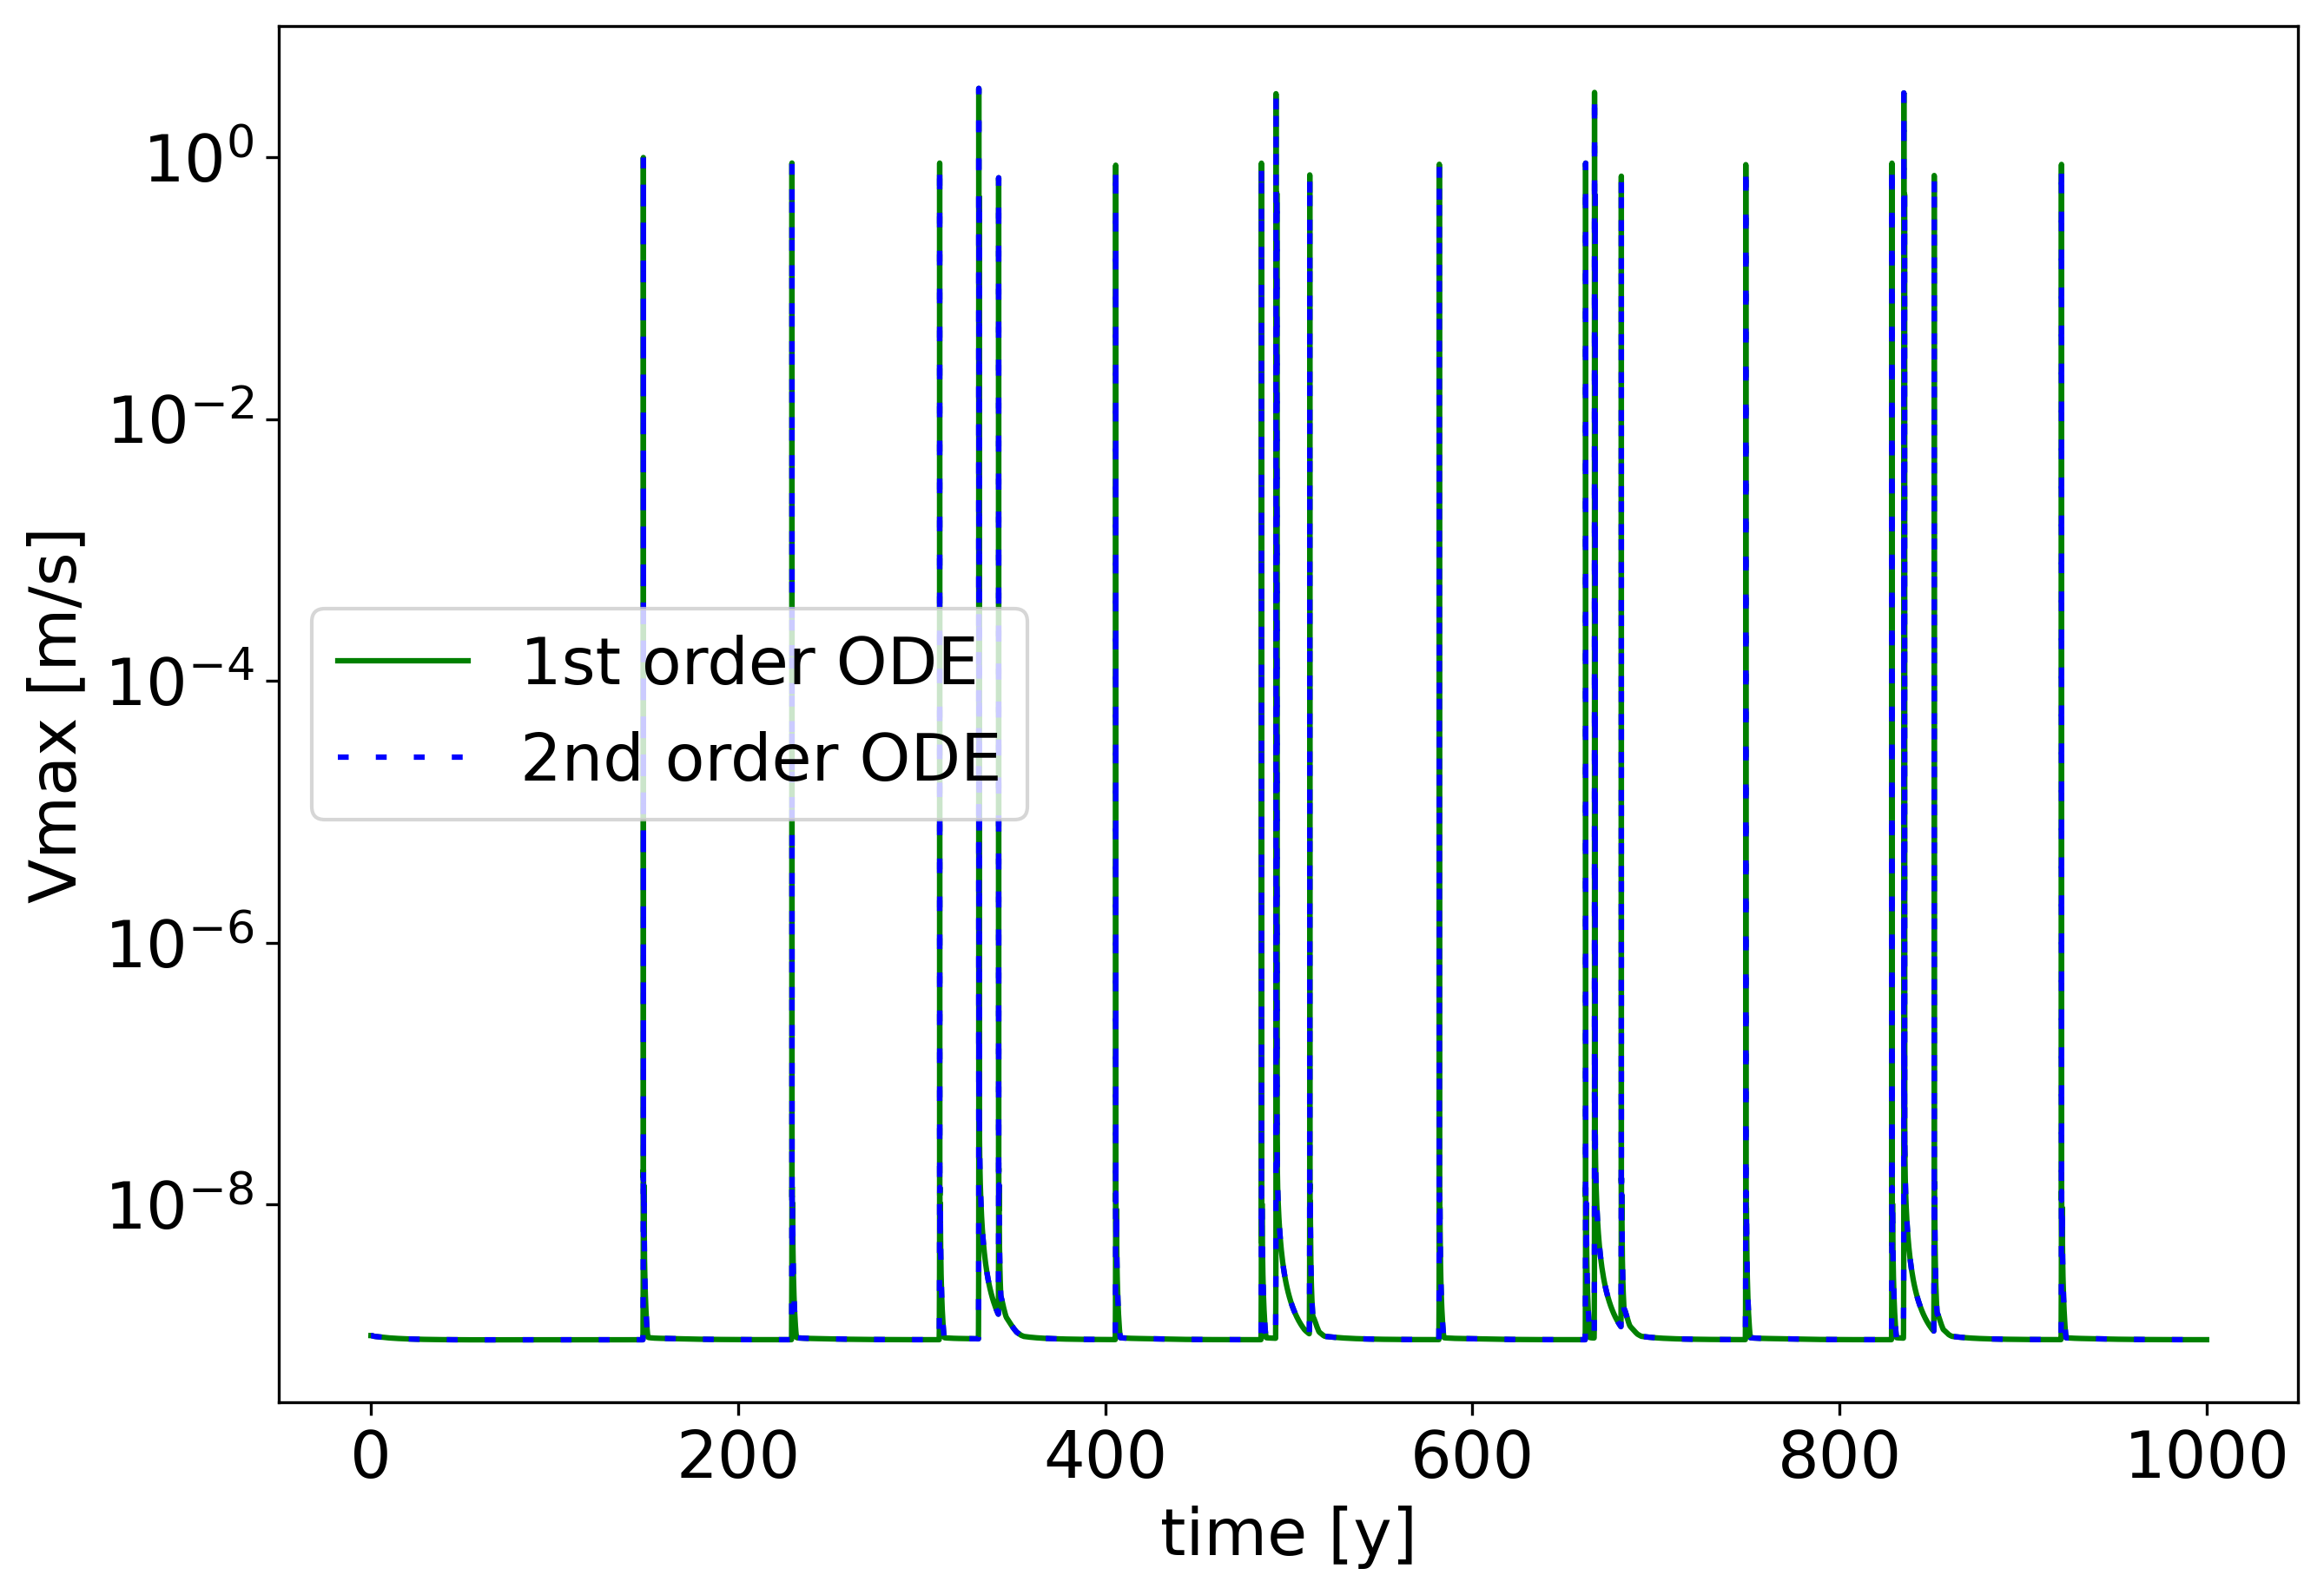
\includegraphics[width=0.45\textwidth]{images/TANDEMtimeEvolutionVExtendedODE1stvs2ndOrder.png}
	\caption{Maximum slip rate in the 1st and 2nd order formulations on a domain with 5 fault elements for 1000 years} 
	\label{fig:timeEvolution_2ndOrderODE_vs_1stOrderODE}
\end{figure}

\subsection{Derivation of the analytic Jacobian}
The Jacobian of the second order ODE formulation in \autoref{eq:2nd_order_ODE_formulation} has components in the slip $S$, the state variable $\psi$ and in the slip rate $V$. The block structure is given by:
\begin{equation}
\label{eq:Jacobian_2nd_order_ODE_formulation}
	\mathbf{J}_{S_j,\psi_j,V_j}F_i(S,\psi,V) = 	\begin{pmatrix}
	\pdv{V_i}{S_j} 				& \pdv{V_i}{\psi_j}	 			& \pdv{V_i}{V_j} \\
	\pdv{g_i(\psi,V)}{S_j} 		& \pdv{g_i(\psi,V)}{\psi_j}	 	& \pdv{g_i(\psi,V)}{V_j} \\
	\pdv{h_i(t,\psi,V)}{S_j} 	& \pdv{h_i(t,\psi,V)}{\psi_j} 	& \pdv{h_i(t,\psi,V)}{V_j}
\end{pmatrix}
\end{equation}
It can be directly seen that none of the terms $V$, $g$ and $h$ depend on the slip $S$, therefore all entries in the first column of block matrices evaluate to 0. A direct consequence is the singularity of the Jacobian matrix, which makes it unsuitable for the Newton iteration. Under consideration of all 0-entries, the matrix takes the form, where $\mathbf{K}$ is invertible with a partial diagonal structure:
\begin{equation}
\label{eq:Jacobian_2nd_order_ODE_formulation_with_zeros}
\mathbf{J}_{S_j,\psi_j,V_j}F_i(S,\psi,V) = 	\begin{pmatrix}
\mathbf{0} 												& \begin{matrix}\mathbf{0} & \mathbf{I} \end{matrix} \\
\;\,\begin{matrix}\mathbf{0} \\ \mathbf{0} \end{matrix} & \mathbf{K} 	\\
\end{pmatrix}
\end{equation}

To cope with this issue, recall that $g$ and $h$ do not depend on $S$, it is thus possible to apply the Newton iteration only on $\psi$ and $V$ with the reduced Jacobian $\mathbf{K}$. Once the slip rate $V^{(n+1)}$ is known for the next timestep, the implicit scheme can be directly applied to $S$ without the need to solve a nonlinear system of equations. Indeed, the value of the right-hand side of the ODE at the next timestep for $\dot{S^{(n+1)}} = V^{(n+1)}$ is directly available and can be plugged in the BDF scheme. If $S^{(n-i)}$ are the solutions at the $i$ previous timesteps, $\alpha_{n-i}$ the time adaptive BDF coefficients at these steps and $\sigma$ the current shift, the new slip rate $S^{(n+1)}$ can be calculated as: 
\begin{equation}
	\label{eq:update_S_2ndOrderODE}
	S^{(n+1)} = \frac{1}{\sigma}\left(V^{(n+1)} - \sum_{i=0}^{k}\alpha_{n-i}S^{(n-i)}\right)
\end{equation}

For the remaining unknown Jacobian $\mathbf{K}$, the entries in the first line are identical to the partial derivatives $\pdv{g}{\psi}$ and $\pdv{g}{V}$ \autoref{eq:Jacobian_DAE_formulation} and are trivial to compute. The entries in the second line are more challenging to obtain as they describe the variation of the product and sum of other Jacobian matrices. \\

We start from the expression for $h$ in \autoref{eq:2nd_order_ODE_formulation_sum_of_Jacobians} and introduce the new variables $C = \pdv{f}{t}$, a constant vector from the partial time derivative, $\mathbf{A} = \pdv{f}{S}$, a constant and dense matrix from the DG discretization defined in \autoref{eq:partialDerivative_df_dS}, and $\xi(\psi,V) = \left(\pdv{f}{V}\right)^{-1}$ and $\zeta(\psi,V) = \pdv{f}{\psi}$, two diagonal matrices which depend on the state variable and the slip rate. With these new variables, the components of $h$ can be expressed as:
\begin{equation}
	h_i = -\xi_{ii}\left(C_i + \mathbf{A}_{ik}V_k + \zeta_{ii}g_i\right)
\end{equation}
The first partial derivative $\pdv{h_i}{S_j}$ can be directly evaluated to 0 since none of the terms depends on the slip $S$. Next, the derivative with respect to the slip rate is already more complex:
\begin{align}
	\pdv{h_i}{\psi_j} &= -\left[\pdv{\xi_{ii}}{\psi_j}\left(C_i + \mathbf{A}_{ik}V_k + \zeta_{ii}g_i\right) + \xi_{ii}\left(\pdv{\zeta_{ii}}{\psi_j}g_i + \zeta_{ii}\pdv{g_i}{\psi_j}\right)\right]\delta_{ij}
\end{align}
The derivatives of $\xi$ and $\zeta$ can be directly computed from Equations \ref{eq:partial_df_dpsi} and \ref{eq:partial_df_dV}:

\begin{align}
	\pdv{\xi_{ii}}{\psi_j} &= \frac{2V_0\sigma_n e^{\frac{\psi_i}{a}}}{\sqrt{\frac{e^{\frac{2\psi_i}{a}}V_i^2}{4V_0^2}+1}\left(2V_0\eta\sqrt{\frac{e^{\frac{2\psi_i}{a}}V_i^2}{4V_0^2}+1}+a\sigma_n e^{\frac{\psi_i}{a}}\right)^2}\delta_{ij} \\
	\pdv{\zeta_{ii}}{\psi_j} &= -\frac{\sigma_nV_ie^{\frac{\psi_i}{a}}}{2aV_0\left(\frac{e^{\frac{2\psi_i}{a}}V^2}{4V_0^2}+1\right)^{\frac{3}{2}}}\delta_{ij}
\end{align}

The last derivative with respect to the slip rate $V$ is not a diagonal matrix anymore:
\begin{align}
	\pdv{h_i}{V_j} &= -\left[\pdv{\xi_{ii}}{V_j}\left(C_i + \mathbf{A}_{ik}V_k + \zeta_{ii}g_i\right)\delta_{ij} + \xi_{ii}\left(\mathbf{A}_{ij} + \pdv{\zeta_{ii}}{V_j}g_i\delta_{ij} + \zeta_{ii}\pdv{g_i}{V_j}\delta_{ij}\right)\right]
\end{align}
Again, the unknown derivatives can be calculated:
\begin{align}
	\pdv{\xi_{ii}}{V_j} &= -\frac{a\sigma_n V_ie^{\frac{3\psi_i}{a}}}{2V_0\sqrt{\frac{e^{\frac{2\psi_i}{a}}V_i^2}{4V_0^2}+1}\left(2V_0\eta\sqrt{\frac{e^{\frac{2\psi_i}{a}}V_i^2}{4V_0^2}+1}+a\sigma_n e^{\frac{\psi_i}{a}}\right)^2}\delta_{ij} \\
	\pdv{\zeta_{ii}}{V_j} &= -\frac{\sigma_n e^{\frac{\psi_i}{a}}}{2V_0\left(\frac{e^{\frac{2\psi_i}{a}}V_i^2}{4V_0^2}+1\right)^{\frac{3}{2}}}\delta_{ij}
\end{align}
By now, all components to set up the Jacobian matrix in \autoref{eq:Jacobian_2nd_order_ODE_formulation} are provided and the formulation is ready to be used with implicit methods. \\
In the implementation, the singularity is handled slightly differently: solving the Newton iteration with the matrix $\mathbf{K}$ in \autoref{eq:Jacobian_2nd_order_ODE_formulation_with_zeros} would require to copy the entries for $V$ and $\psi$ from the solution vector to another vector whose size matches the dimensions of $\mathbf{K}$. Instead, $\mathbf{K}$ is extended with ones on the diagonal elements related to the $S$, and in each Newton step, just before solving the linear system, the corresponding entries in the right-hand side vector are set to zero. As such, the change in $S$ always vanishes and the convergence of the Newton iteration is not altered. After a successful termination, the entries for $S$ are updated as described in \autoref{eq:update_S_2ndOrderODE}.

\section{Numerical Aspects and Implementation Details}
So far, 4 different methods have been proposed, which can be solved explicitly or implicitly. An overview of the available is given in \autoref{tab:availableMethods}, which in addition states the length of the solution vector. Methods with a size $2n$ contain the slip $S$ and the state variable $\psi$ in the solution vector, and methods with $3n$ contain in addition the slip rate $V$.
\begin{table}[H]
	\centering 
	\begin{tabular}{ | c | c c | c |}
		\hline	
						& explicit	& implicit 	& Vector length\\ \hline
		1st order ODE 	& yes 		& yes 		& 2$n$\\  
		extended DAE  	& no 		& yes 		& 3$n$\\
		compact DAE  	& no 		& yes 		& 2$n$\\
		2nd order ODE  	& yes 		& yes 		& 3$n$\\
		\hline
	\end{tabular}
	\caption{Overview of the available methods}
	\label{tab:availableMethods}
\end{table}
This section provides more details about the necessary components to solve each of these methods numerically. The focus is first on adaptive time integration methods followed by a discussion about the proper definition of tolerances. Next, the Newton iteration and its convergence properties is described to solve the nonlinear systems which arise in the implicit problem formulations. Finally, the data layout is described along with a quick estimate of the memory requirements for each problem formulation. In addition, the section exposes the peculiarities and possible limitations of the respective methods.

\section{Time integration}
The PETSc environment is used to handle most of the time integration. Among all available integrator, the new code is only compatible with Runge-Kutta methods for explicit formulations and BDF methods for implicit formulations. \\
For the explicit methods, the 2nd order Bogacki-Shampine scheme with a 3rd order error estimate and the 4th order Dormand-Prince scheme with a 5th order error estimate will be compared later in the results section. Their respective Butcher tableaus are given in /:TODO////---APPENDIX-----////. \\
For now, only the basic PETSc timestep adapter is used. The next timestep size is calculated in function of the estimation of the local truncation error $\epsilon$ and of the order of the estimate $\bar{k}$. In general, $\bar{k}=k+1$, where $k$ is the order of the numerical scheme. 
\begin{equation}
	h_{n+1} = C\epsilon^{-1/\bar{k}}h_n
\end{equation}
The safety factor $C$ is set to 0.9, and the scaling from one timestep to another is restricted to values between 0.1 and 10. In the native PETSc implementation for BDF, this upper bound for the factor is set to 2, but this only matters for the very first timesteps, since the relative change between timestep sizes is generally below 2 afterwards.

\subsection{Implementation of the BDF schemes}
For the implicit methods, any BDF scheme of order 1 to 6 can be used. For the first few timesteps, not all necessary previous solutions are available yet to perform a $k$-order scheme. In this case, the highest possible order is used until the order $k$ is reached. If for example, a 4th order BDF scheme is required, the first three steps will be actually performed with the respective orders 1, 2 and 3. \\
The native PETSc error estimate uses the Lagrangian polynomials as described in \autoref{sssec:errorEstimateBDFLagrange}. The second method with an embedded higher order execution of the BDF scheme from \autoref{sssec:errorEstimateBDFEmbeddedScheme}, was manually implemented and the user can choose between both possibilities. Again, in the first few steps, the solution vectors are not yet available to execute the BDF scheme of order $k+1$ for the error estimate. In this case, the error is evaluated with a lower order scheme $k-1$ until enough old solution vectors are available. \\
Further, the adaptive BDF order finding from \autoref{sssec:adaptiveBDFOrder} has been implemented and is used if the user provided "0" for the BDF order. 

\subsection{Switching between different methods}
The simulation supports the use of different solvers and time integration methods for the aseismic slip phase and for the earthquake phase. To detect in which phase the simulation is currently in, the maximum slip rate $V_{max}$ at the current timestep is compared to the environment slip $V_0$. If $V_{max}>V_0$ is verified, it means that the simulation is currently in an earthquake, else wise it is in the aseismic slip. When the simulation detects a switch from one state to the other, and if a different problem formulation or integration method is defined by the users for both states, the program overwrites the PETSc configuration and restarts the solver at the current timestep with the new methods. It is thus possible, for instance, to use the compact DAE formulation for the aseismic slip and the 2nd order ODE formulation with an explicit Runge-Kutta scheme for the earthquake. 

\subsection{Tolerances for the time integration}
Tolerances play a crucial role fort adaptive time-stepping methods. A proposed timestep is accepted only if the estimated error is inferior to a defined tolerance $t$, therefore a carefully chosen tolerance has a direct impact on the timestep size and consequently on the total number of time iterations to reach the final simulation time. If $u_i$ refers to all components of the solution vector and $u_i^{(e)}$ to the components of the embedded solution used for the error estimate, then a step is acceptable if following condition is fulfilled: 
\begin{equation}
\left\|\frac{u_i - u_i^{(e)}}{t_i}\right\|_\infty = \max_i \left|\frac{u_i - u_i^{(e)}}{t_i}\right|
\quad \leq \quad 1
\end{equation}
The infinity norm is used because a too large deviation in one node of the fault can erroneously provoke an earthquake at a too early time and thus strongly affects the accuracy of the results for the whole system. If the 2-norm was used, as it is common for other applications, too large errors at some nodes may occur, which are then compensated by nodes where the actual and the embedded solutions match well. \\

The tolerance $t_i$ can be defined independently for each component of the solution vector. It is calculated for each time step with an absolute tolerance $t_i^a$ and a relative tolerance $t_i^r$. 
\begin{equation}
t_i = t_i^a + \max\left(u_i,u_i^{(e)}\right)t_i^r
\end{equation}
Since some components of the solution vector correspond to the values of the state variable $\psi$ and the other components correspond to the slip $S$, it is appropriate to use two different tolerances for the respective quantities. Thus, $t_i^a$ and $t_i^r$ take the values $t_\psi^a$ and $t_\psi^r$ for the components in $\psi$, the values $t_S^a$ and $t_S^r$ for the slip, and, for the 2nd order ODE, $t_V^a$ and $t_V^r$ for the slip rate. As seen in \autoref{fig:EvolutionAllQuantitiesMinMaxStacked200Elements}, the slip increases steadily over the simulation time. A relative tolerance does not make a lot of sense here, because the difference between the maximum and minimum slips are relevant for the simulation and not its magnitude. A relative tolerance would be effectively less strict after many timesteps, whereas a carefully chosen absolute tolerance keeps the accuracy. The state variable remains at values in the range $[0.4, 0.8]$ throughout the simulation, so either an absolute or a relative tolerance or both can be defined. The slip rate also remains within a range of values, but the large difference between the aseismic slip, where $V=10^{-9}$m/s, and the earthquake with $V_{max}=5m/s$, indicates that a relative tolerance is appropriate, combined with an eventual absolute tolerance. 

\subsubsection{Lower bound for the tolerances}
\label{ssec:LowerBoundTimeTolerance}
For the 1st order ODE and both DAE formulations, the slip $S$ and the state variable $\psi$ are integrated over time and thus require tolerances. To get an idea about the range of values they can take, we estimate the smallest local truncation error in  $S$ and $\psi$ that can be achieved at all. For that, we use the fact that the friction law can only be calculated iteratively up to an error $\varepsilon_{max} < 10^{-12}$ and we assume that in the worst case this error propagates entirely to the slip $S$ or to the state variable $\psi$. The impact of a perturbation $\varepsilon^{\psi}$ or $\varepsilon^{S}$ on the friction law is set to $\varepsilon_{max}$ and is solved with a first order Taylor polynomial.

\begin{align}
&\begin{cases}
	\varepsilon_{max} < f(S+\varepsilon^{S},\psi,V) - f(S,\psi,V) \\
	\varepsilon_{max} < f(S,\psi+\varepsilon^{\psi},V) - f(S,\psi,V) 
\end{cases} &&
\Leftrightarrow&
&\begin{cases}
		\varepsilon_{max} < \left|\pdv{f_i}{S_j}\right|\mathbbm{1}_j \varepsilon^S + \mathcal{O}\left(\left(\varepsilon^S\right)^2\right) & \forall i \\[0.2cm]
		\varepsilon_{max} < \left|\pdv{f_i}{\psi_j}\delta_{ij}\right|\varepsilon^\psi + \mathcal{O}\left(\left(\varepsilon^\psi\right)^2\right) & \forall i 
\end{cases} \\
&&&\Leftrightarrow &
&\begin{cases}
	\varepsilon^S > \left[\min_i\left|\pdv{f_i}{S_j}\right|\mathbbm{1}_j\right]^{-1}\varepsilon_{max}  \\[0.2cm]
	\varepsilon^\psi > \left|\frac{\sigma_n}{2V_0}\frac{V_i e^{\frac{\psi_i}{a}}}{\sqrt{\frac{e^{2\psi_i/a}V_i^2}{4V_0^2} + 1}} \right|^{-1}\varepsilon_{max} & \forall i
\end{cases}
\end{align}
In the first condition, $\mathbbm{1}$ denotes the one vector, so we try to find the minimum absolute row sum of the constant matrix $\pdv{f}{S}$. A look at the range of the absolute row sums in \autoref{tab:rangeCdotONE} tells that the searched value does not depend of the problem size, so a lower bound for the error in $S$ can be conveniently calculated by $\varepsilon^S > \varepsilon_{max}/0.257=4\cdot10^{-12}$.
\begin{table}[H]
	\centering 
	\begin{tabular}{ | c | c c c c c |}
		\hline	
		Number of fault elements	& 21 	& 40 	& 80 	& 200 	& 400 	\\ \hline
		Maximum absolute row sum    & 62.3	& 129	& 283	& 624 	& 1230	\\  
		Minimum absolute row sum  	& 0.257	& 0.257 & 0.257	& 0.257 & 0.257 \\
		\hline
	\end{tabular}
	\caption{Range of the components in $\pdv{f_i}{S_j}\mathbbm{1}_j$ for different problem sizes} 
	\label{tab:rangeCdotONE}
\end{table}

In the second condition, the lower bound of the exponential term in the denominator $e^{2\psi_{min}/a_{max}} = e^{2 \cdot 0.5 / 0.025} \approx 5.5\cdot10^{34}$ is already extremely high, so that the term $+1$ can be neglected in the square root. Then, the expression simplifies dramatically as $\pdv{f}{\psi} \approx \sigma_n = 50$, which can be safely used for the lower bound of the error in $\varepsilon^\psi > \varepsilon_{max}/50 = 2\cdot10^{-14}$. \\
For the second order ODE, the tolerance in $V$ is also required, so the same procedure is applied to determine a lower bound for the error term $\varepsilon^V$.
\begin{align}
	&\varepsilon_{max} < f(S,\psi,V+\varepsilon^{V}) - f(S,\psi,V)
	&&\Leftrightarrow&&
	\varepsilon_{max} < \left|\pdv{f_i}{V_j}\delta_{ij}\right|\varepsilon^V + \mathcal{O}\left(\left(\varepsilon^V\right)^2\right) & \forall i \\
	&&&\Leftrightarrow &&
	\varepsilon^V > \left|\frac{\sigma_n}{2V_0}\frac{ e^{\frac{\psi_i}{a}}}{\sqrt{\frac{e^{2\psi_i/a}V_i^2}{4V_0^2} + 1}} + \eta\right|^{-1}\varepsilon_{max} & \forall i
\end{align}
With the same approximation as earlier for the denominator, the expression simplifies to $\varepsilon^V > V_i\varepsilon_{max}/(\sigma_n + V_i\eta)$. As opposed to $\varepsilon^S$ and $\varepsilon^\psi$, the error depends on the maximum slip rate in the current iteration, which is in line with the postulate from the previous section that a relative tolerance definition for the slip rate is more appropriate. Sadly, the expression for the lower bound of $\varepsilon^V$ is not an affine function and can not be used as such as a tolerance. Instead, we can use the condition $\varepsilon^V > V_i\varepsilon_{max}/\sigma_n$, which is still a very accurate lower bound for most of the encountered slip rates. As seen in \autoref{fig:LowerBoundErrorEstimateV}, only for very high slip rates that occur at the peak of an earthquake, the linearized lower bound for $\varepsilon^V$ exceeds significantly the exact value.
\begin{figure}[H]
	\centering
	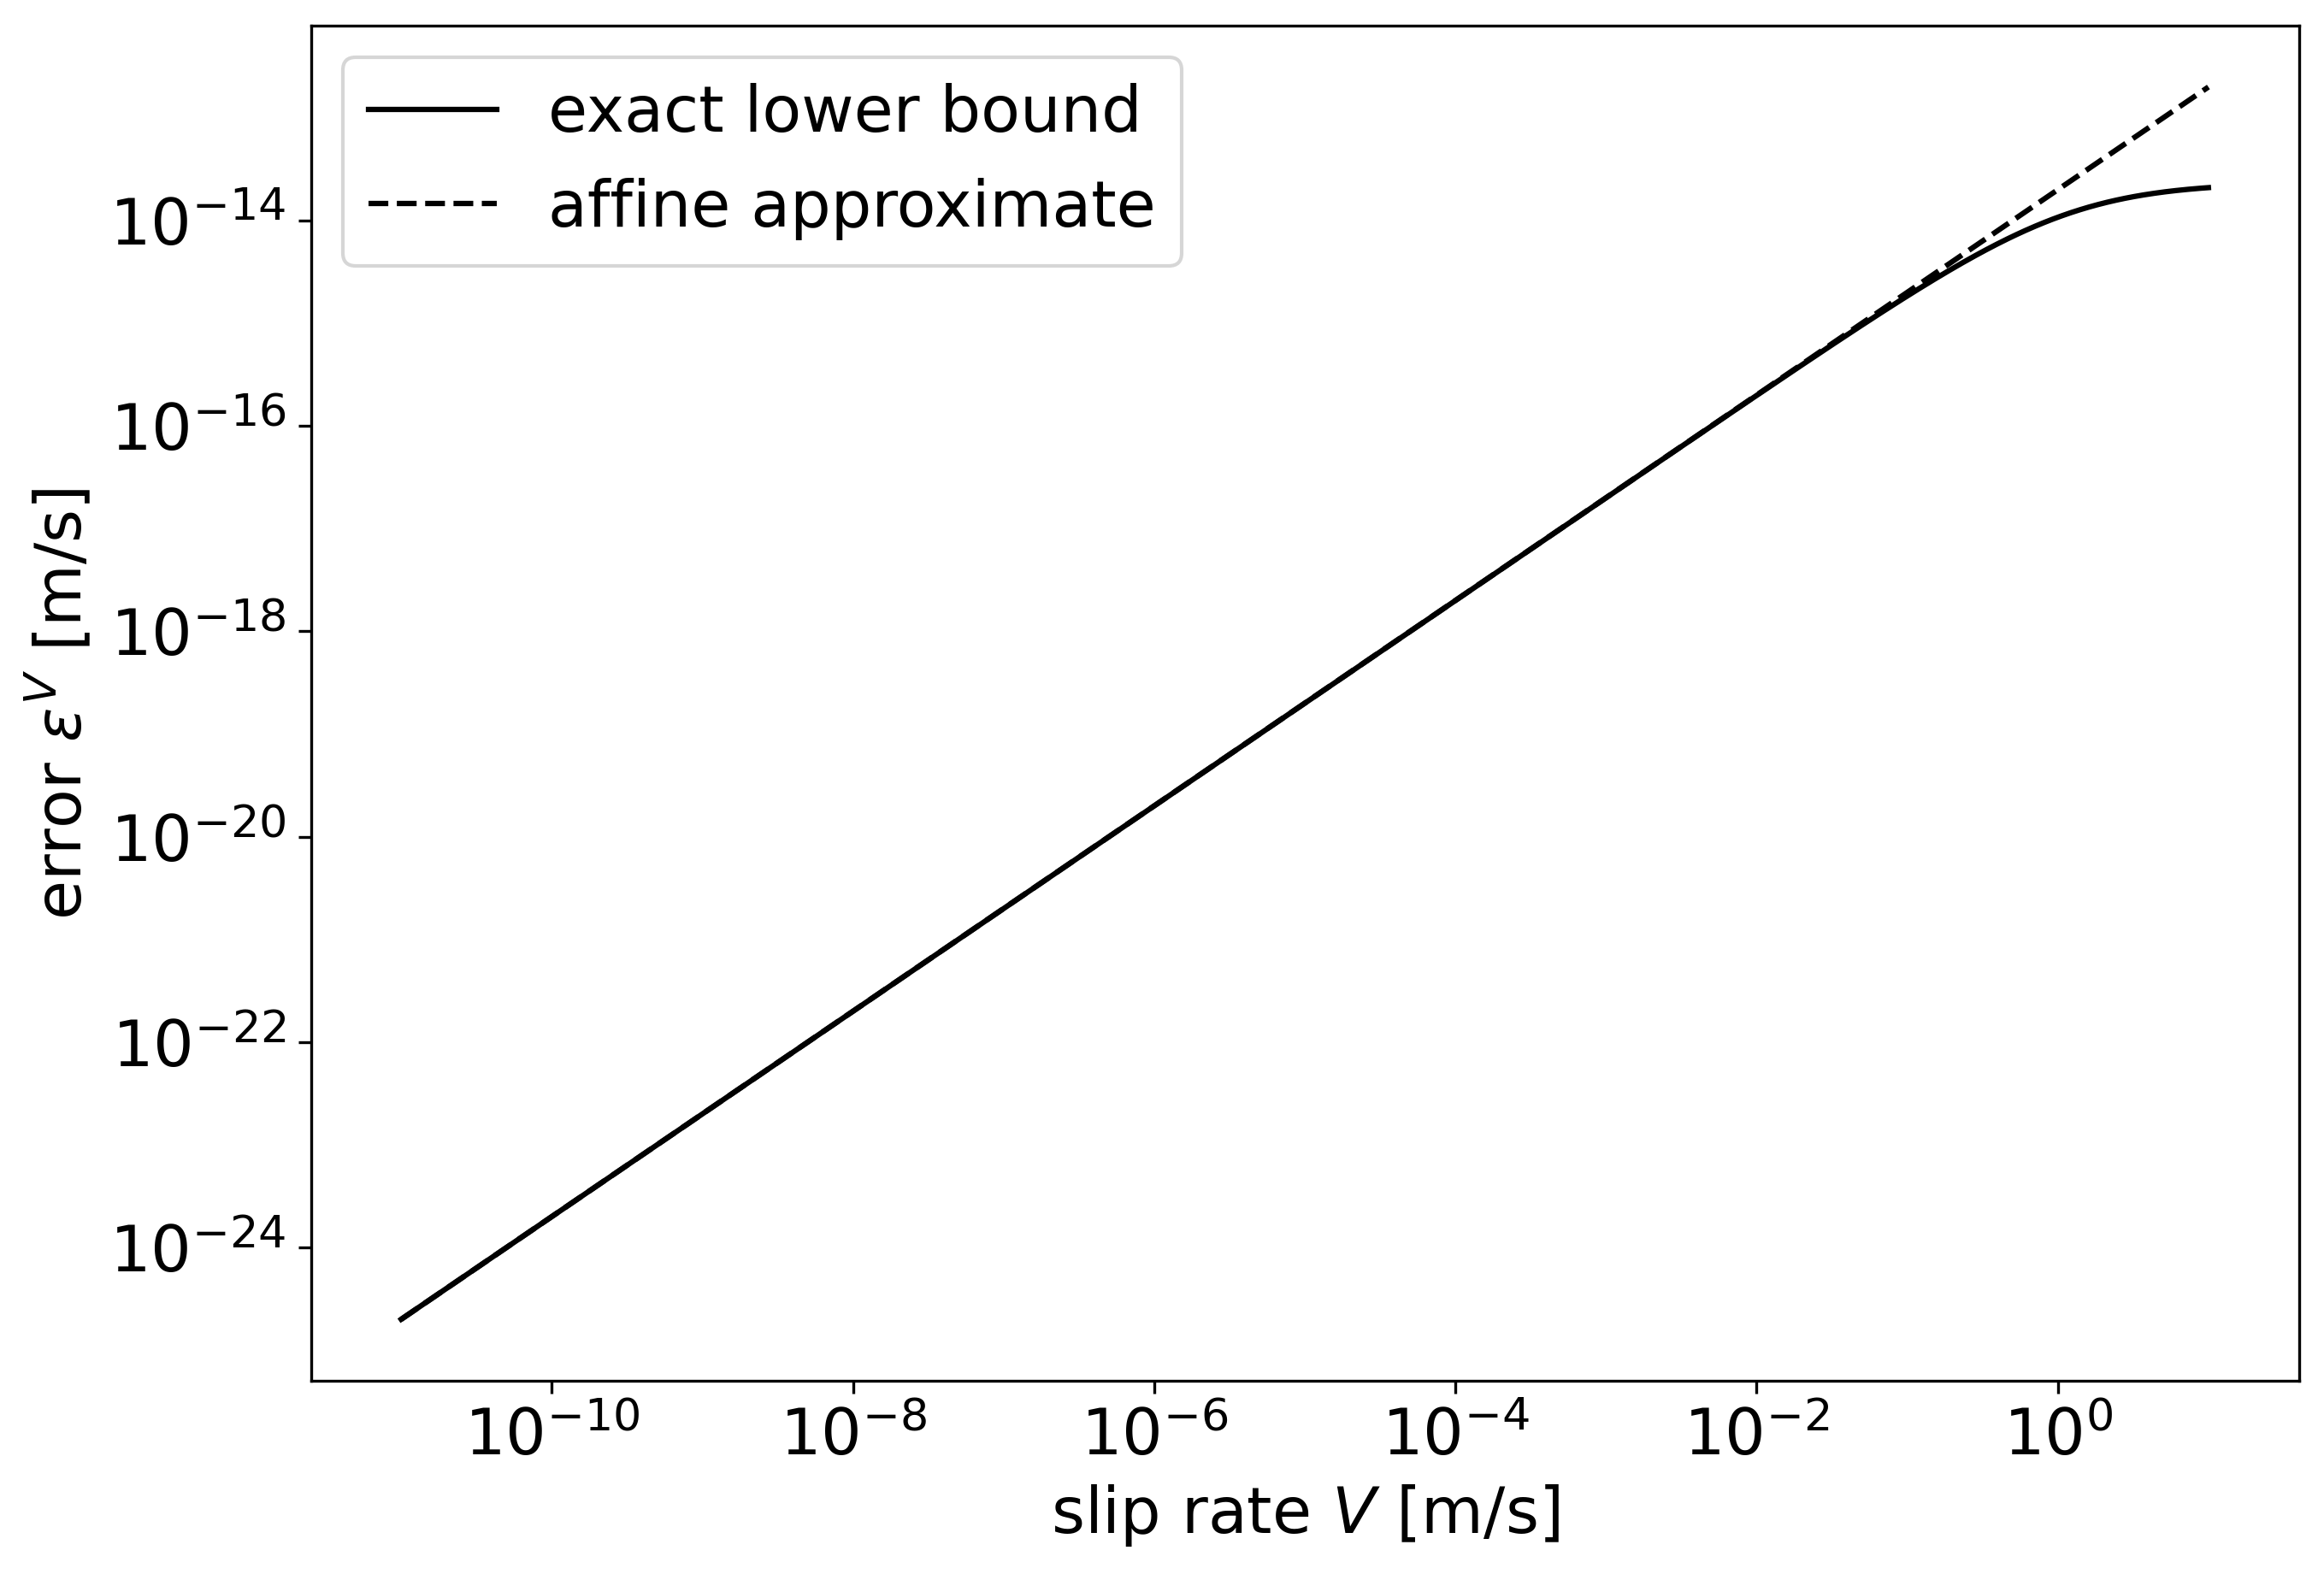
\includegraphics[width=0.5\textwidth]{images/ErrorRelationPSI_VAbsoluteRelative.png}
	\caption{Lower bound for the error in the slip rate $V$ compared to its linear approximate in function of the slip rate}
	\label{fig:LowerBoundErrorEstimateV}
\end{figure}
The proposed tolerances are only of theoretical nature, as they assume that the error only stems from the iterative solver of the friction law. However, the time integration would most likely fail because numerical errors or the sum of the LTE from the different stages of a RK scheme have not been considered. Moreover the error estimate itself is not exact, and, as already discussed in \autoref{ssec:QualityErrorEstimate_0D}, it tend to overestimate the local truncation error, which means that even if the error is within the tolerance, the program would not understand it as such. If one wants to run the simulation with maximal accuracy, it is still wise to add a safety factor to the tolerances.


\section{Newton Iteration}
\label{ssec:ConvergenceNewtonIteration}
The Jacobian matrix is needed to apply implicit numerical methods to the SEAS problem. Unlike explicit methods, they evaluate the right hand side of the ODE with the current solution which is not known yet. To calculate the solution vector at a given time step, a nonlinear algebraic equation of the form $\phi(x) = 0$ needs to be solved where $x$ is the solution vector to be determined. The Newton method is often used to solve the equation because of its ease to implement and its second-order convergence. 

\begin{itemize}
	\item Calculate an initial guess $x_0$
	\item Repeat until tolerance is reached $\|\phi(x_n)\| < TOL$: 
	\begin{itemize}
		\item $x_{n+1} = x_n - J_\phi^{-1}(\phi(x_n)) \phi(x_n)$
	\end{itemize} 
\end{itemize}

The matrix $J_\phi^{-1}(f(x_n))$ is the Jacobi matrix of the function $\phi$ evaluated at the point $x_n$. \\

\subsection{Convergence Properties}
Next, the convergence properties of the Newton iteration with the analytic Jacobian is investigated on the 1st order ODE formulation. For this, we solve one timestep of the implicit Euler method starting from the initial condition of the simulation. The function $\phi$ and its Jacobian matrix are given by: 
\begin{align}
\phi(x) &= -x + x^{(0)} + h F(x) \\
J_\phi(x) &= -I + h J_F(x)
\end{align}
The vector $x$ contains both the components related to the slip $S$ and to the state variable $\psi$ and the right hand-side vector $F(x)$ contains their respective time derivative. The Jacobian of the proposed Newton iteration needs the Jacobian $J_F(x)$ of the right-hand side vector, of which the correctness is evaluated here. The success of the Newton iteration, thus observable second-order convergence, indicates the correctness of the Jacobian matrix. \\
Furthermore, the behavior of the analytic expression of the Jacobian is compared to the behavior of an iterative approximation of it. The Broyden's method \cite{BroydenIteration} provides an enhancement of the Newton method which updates the Jacobian matrix at each iteration without the need of its analytical expression. The main difficulty is to find an appropriate initial guess to achieve a fast convergence. 

\begin{itemize}
	\item Calculate the initial guesses $x_0$ and $J_0$
	\item Repeat until tolerance is reached $\|\phi(x_n)\| < TOL$: 
	\begin{itemize}
		\item $\Delta x_n = x_n - x_{n-1}$ and $\Delta \phi_n = \phi(x_n) - \phi(x_{n-1})$ 
		\item $J_n = J_{n-1} + \frac{\Delta \phi_n - J_{n-1}\Delta x_n}{\|\Delta x_n\|^2} \Delta x_n^T$
		\item $x_{n+1} = x_n - J_n \phi(x_n)$
	\end{itemize} 
\end{itemize}

The motivation behind this update scheme is to minimize the Frobenius norm $\|J_n - J_{n-1}\|_F$. As a matter of simplicity, the initial guess of the Jacobian is obtained with the analytical expression of it, even though its correctness has not yet been shown. Other initialization methods such as finite differences do not lead to convergence of the Broyden method. \\
The experiment has been performed on a symmetric, two-dimensional domain of varying size. The initial guesses for $x$ are obtained with one step of the explicit Euler method with a timestep of $h = 10^5$s. This time step is large enough to obtain an error to the exact value at this time which needs several Newton iterations to be corrected but still small enough to ensure that the Newton iteration converges at all. The evolution of the residual $\phi(x_n)$ is shown in \autoref{fig:convergenceNewtonAndBroydenDifferentSizes}.
\begin{figure}[H]
	\centering
	\begin{subfigure}{0.32\textwidth}
		\centering
		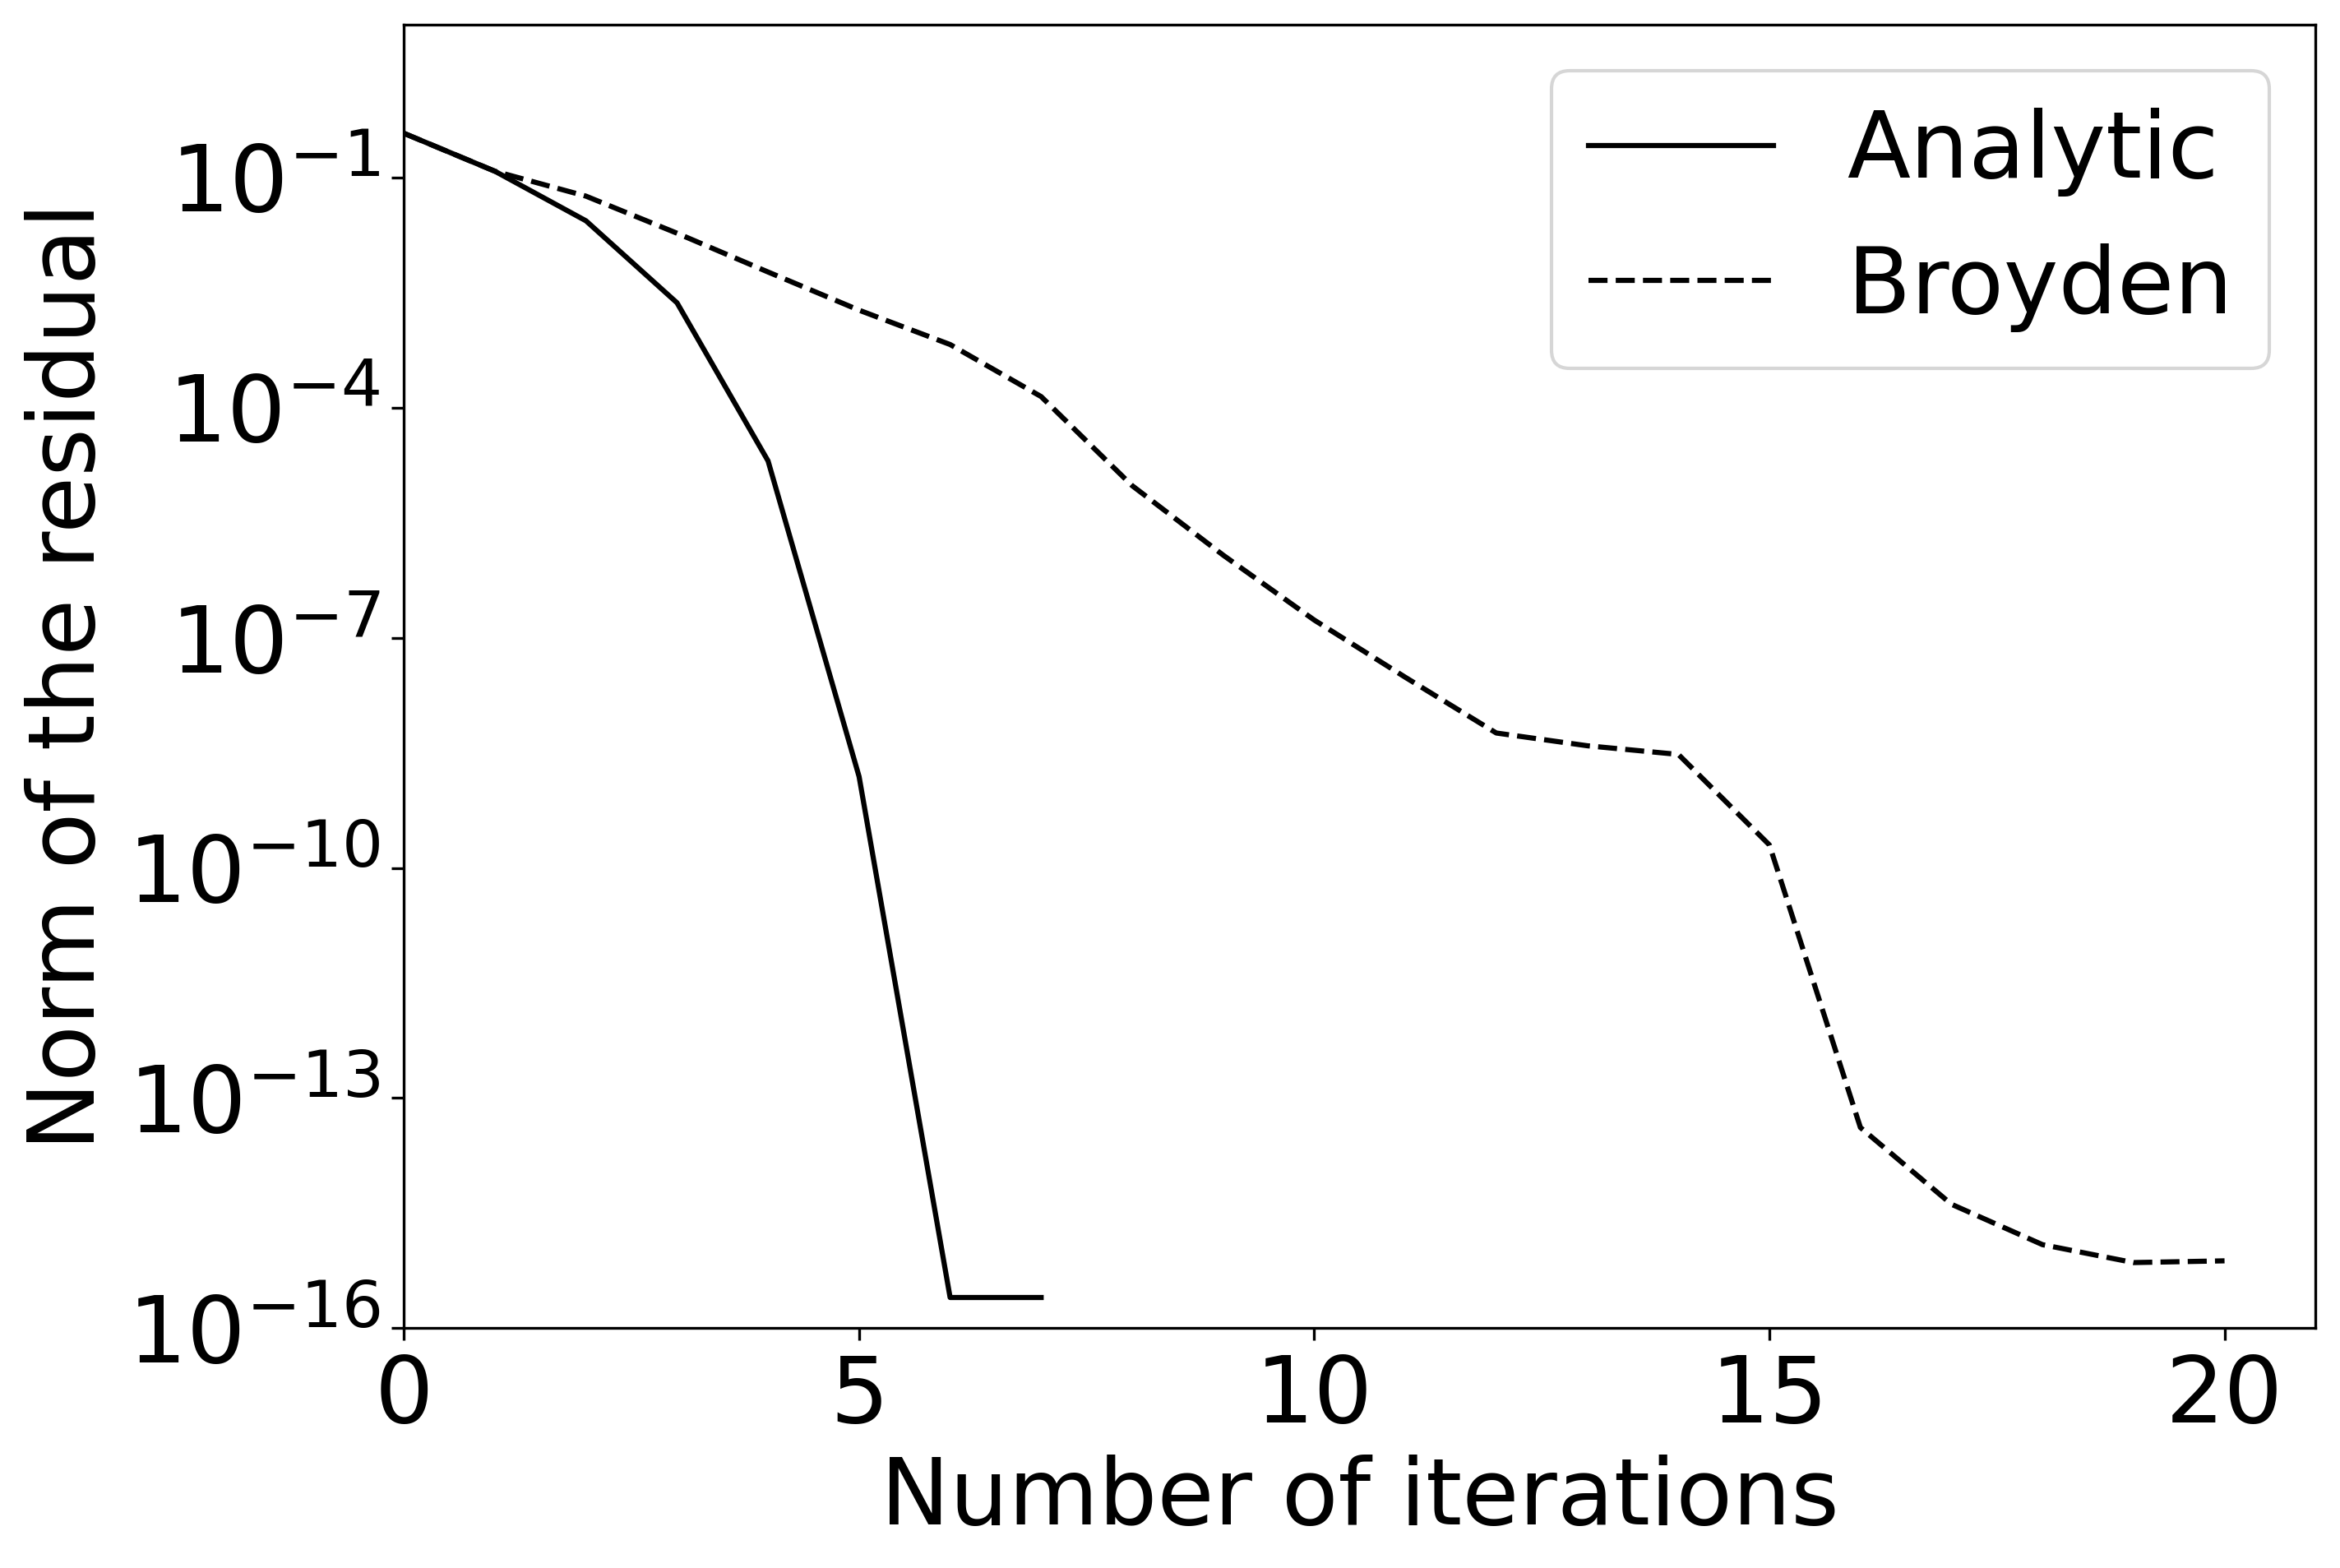
\includegraphics[width=0.9\textwidth]{images/NewtonIterationConvergence5Elements.png}
		\subcaption{5 fault elements} 
	\end{subfigure} 
	\begin{subfigure}{0.32\textwidth}
		\centering
		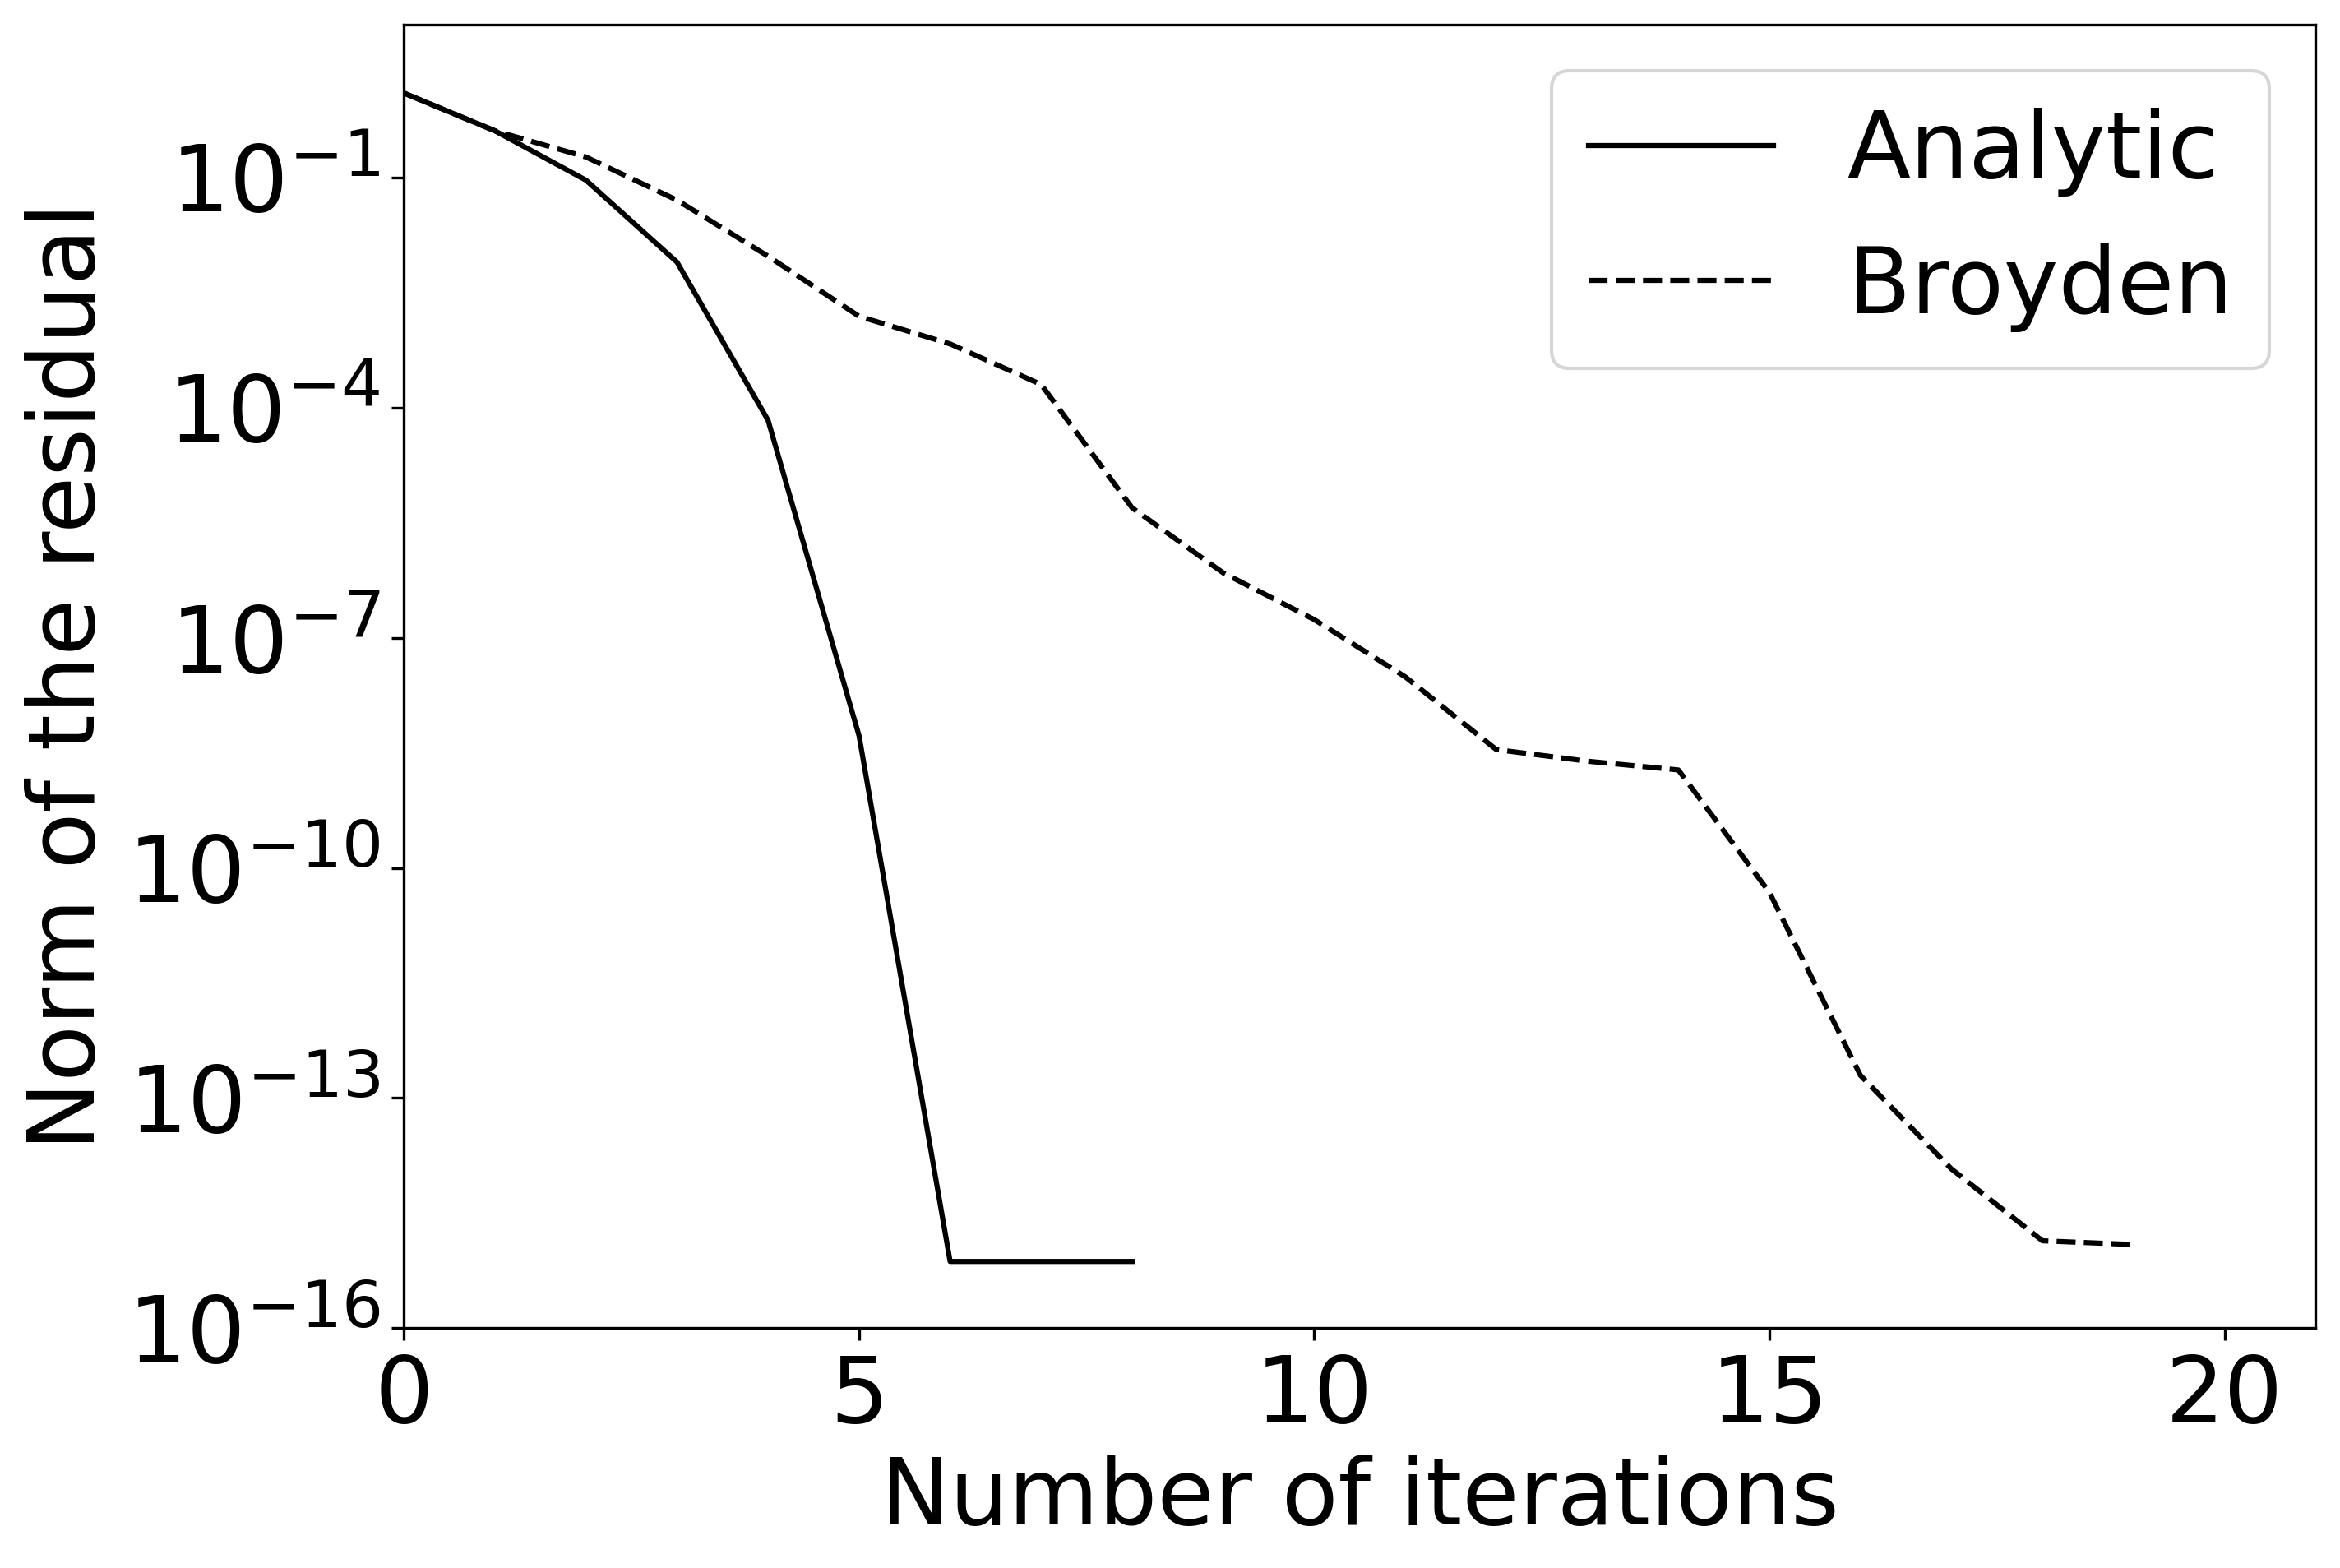
\includegraphics[width=1\textwidth]{images/NewtonIterationConvergence40Elements.png}
		\subcaption{40 fault elements} 
	\end{subfigure}
	\begin{subfigure}{0.32\textwidth}
		\centering
		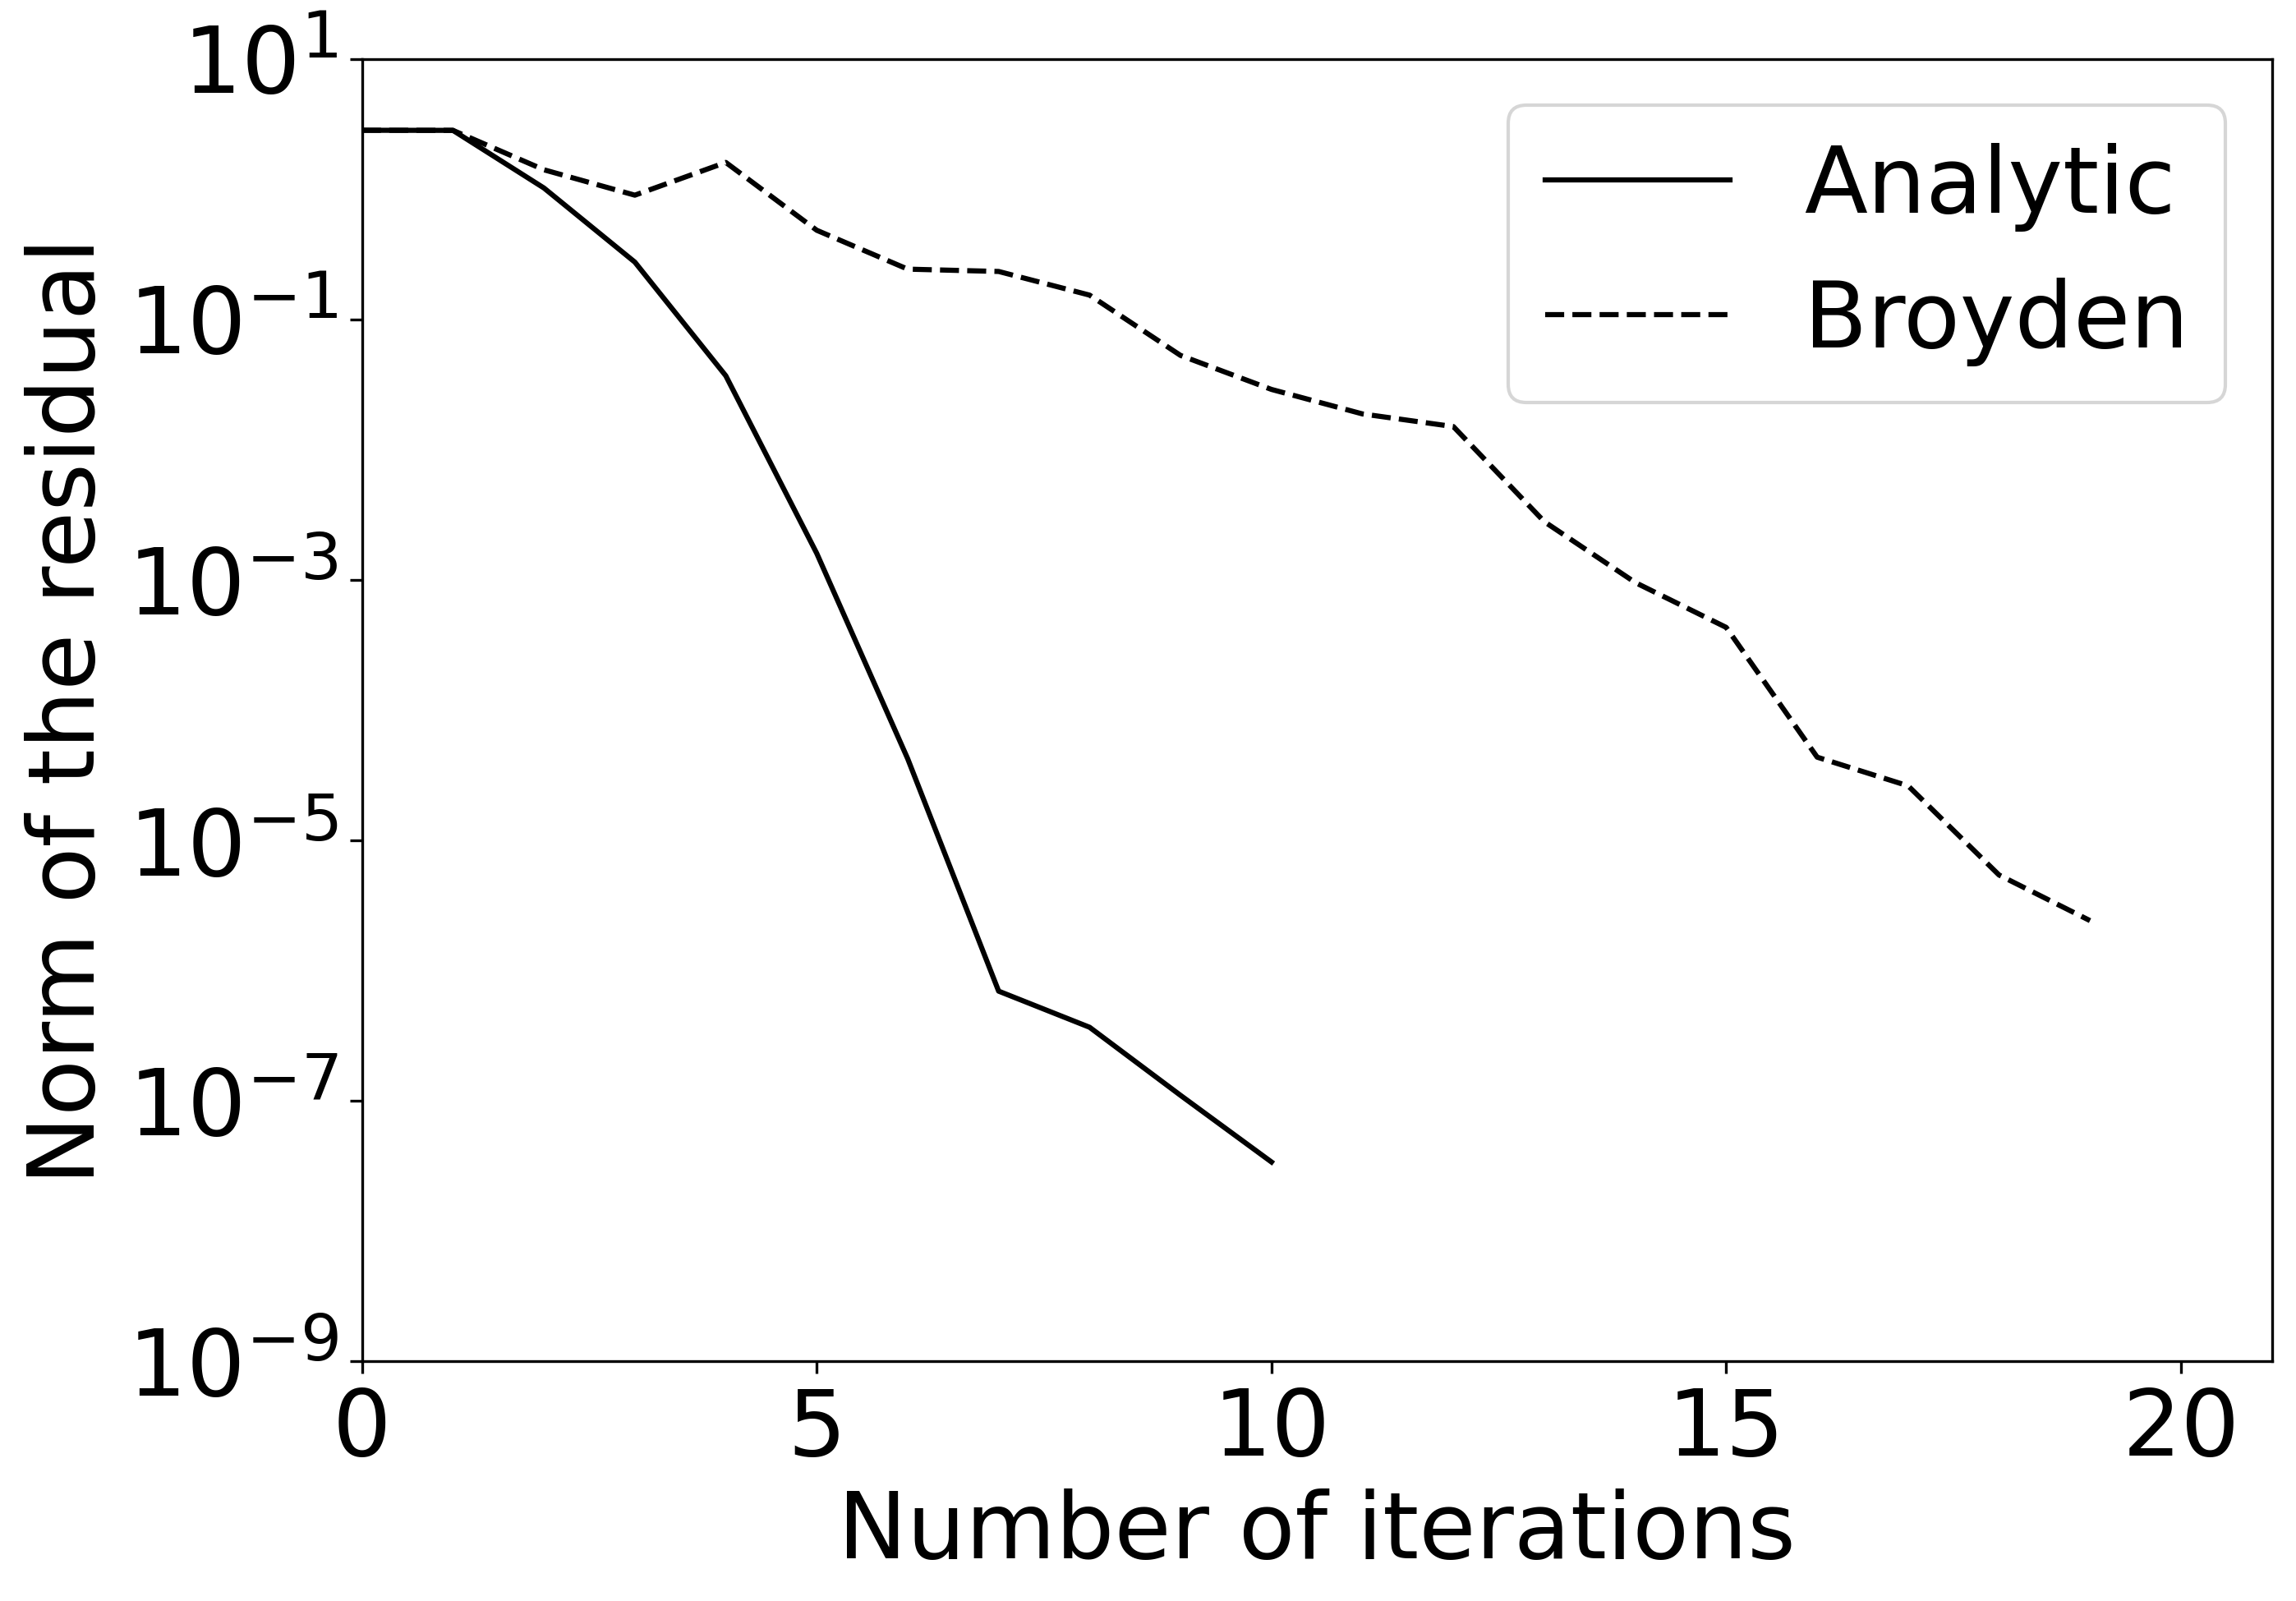
\includegraphics[width=1\textwidth]{images/NewtonIterationConvergence200Elements.png}
		\subcaption{200 fault elements} 
	\end{subfigure}
	\caption{Evaluation of the L2 norm of the residual $\phi(x_n)$ at each iteration of the Newton and Broyden methods}
	\label{fig:convergenceNewtonAndBroydenDifferentSizes}
\end{figure}
It can be immediately seen that the Newton method with an analytic expression of the Jacobian reaches much faster the maximum reachable accuracy of about $10^{-15}$ as if it was approximated with the Broyden method. The convergence rate even seems to be quadratic, as one would expect for the Newton iteration and the convergence is similarly fast for all tested domain sizes. The Broyden method on the other hand shows rather a linear convergence behavior, and the number of needed iterations increases with problem size. This makes the Broyden iteration particularly unsuitable for simulations on large domains. The approximated Jacobian matrix at the end of the Broyden iteration matches with high precision its analytic counterpart, since the maximum relative difference among the entries is of the order of $10^{-5}$. \\
So far, it has been shown that the Newton iteration converges well for various domain sizes. The chosen timestep size $10^5$s is still small, as in the aseismic slip, it may reach the order $10^7$s. \autoref{fig:convergenceNewtonAndBroydenDifferentTimeSteps} shows the norm of the residual for the timestep sizes $10^5$s $10^6$s and $10^7$s. The direct iteration with the analytic Jacobian matrix always has a quadratic convergence, and the slightly higher number of iterations for large timesteps is essentially due to the worse initial guess. In contrast, the Broyden iteration converges much slower if the timestep size increases. 
\begin{figure}[H]
	\centering
	\begin{subfigure}{0.45\textwidth}
		\centering
		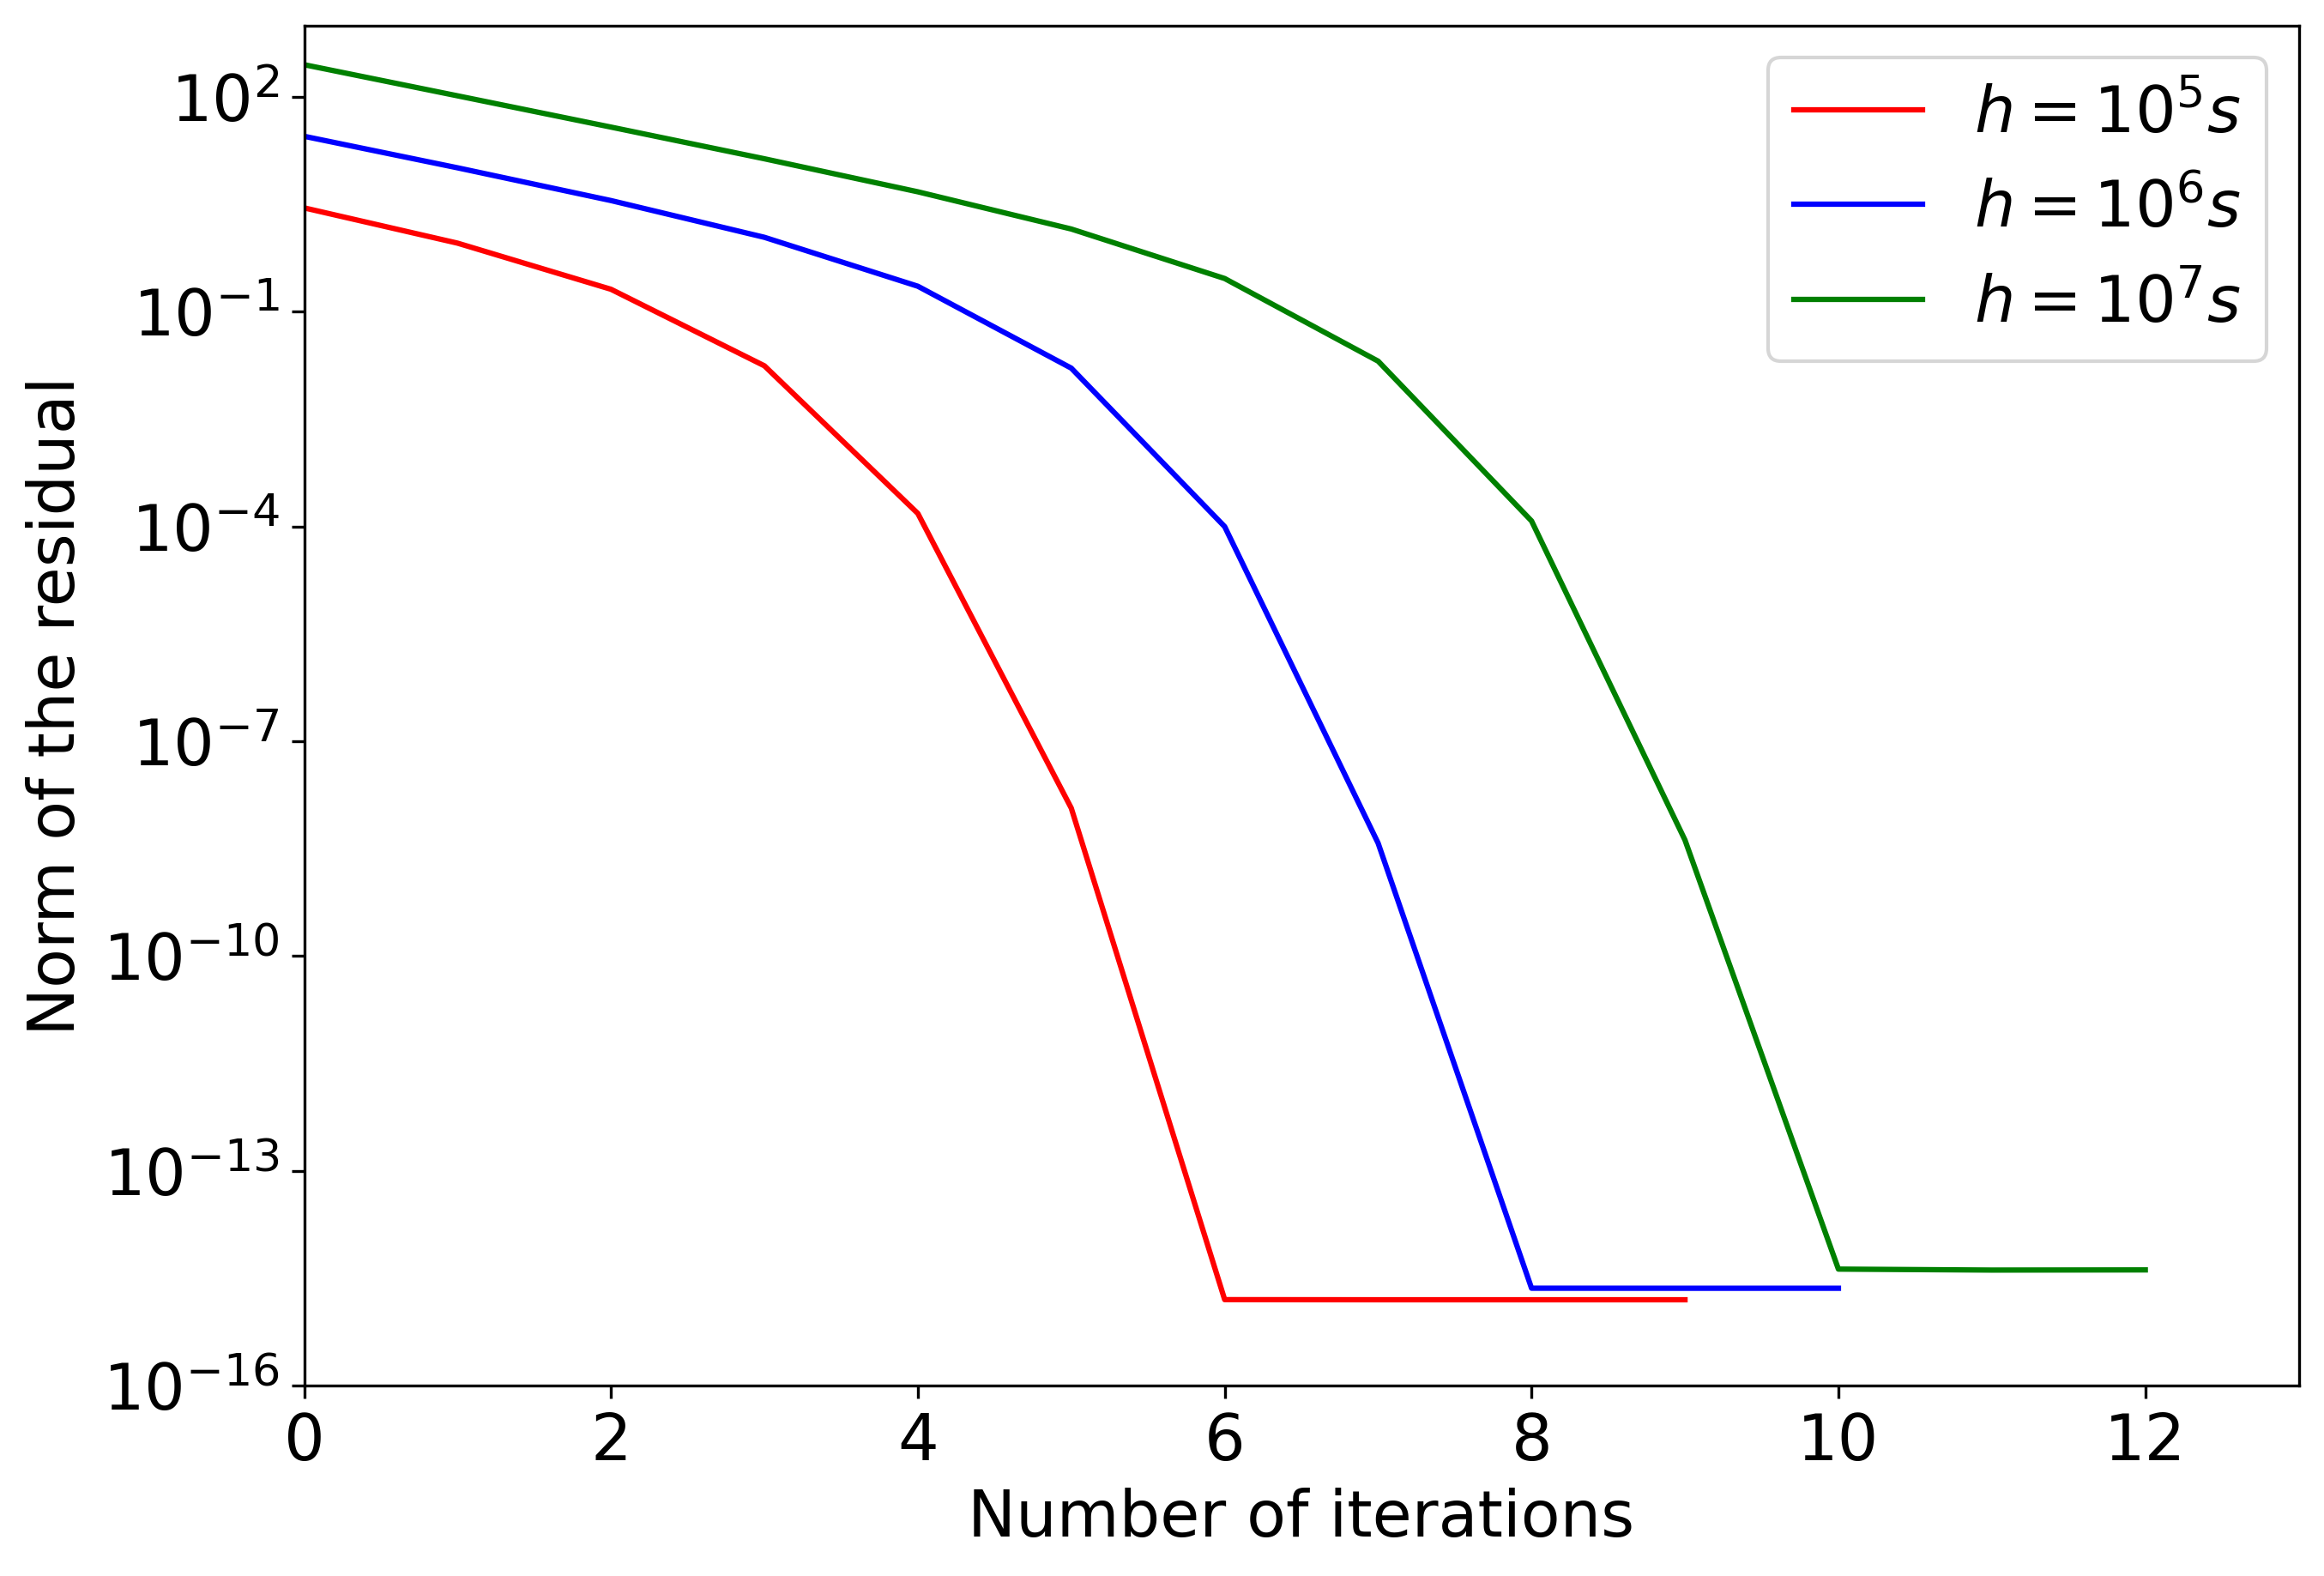
\includegraphics[width=1\textwidth]{images/NewtonIterationConvergence200Elements_DifferentDT_Analytic.png}
		\subcaption{Direct iteration}
	\end{subfigure}
	\begin{subfigure}{0.45\textwidth}
		\centering
		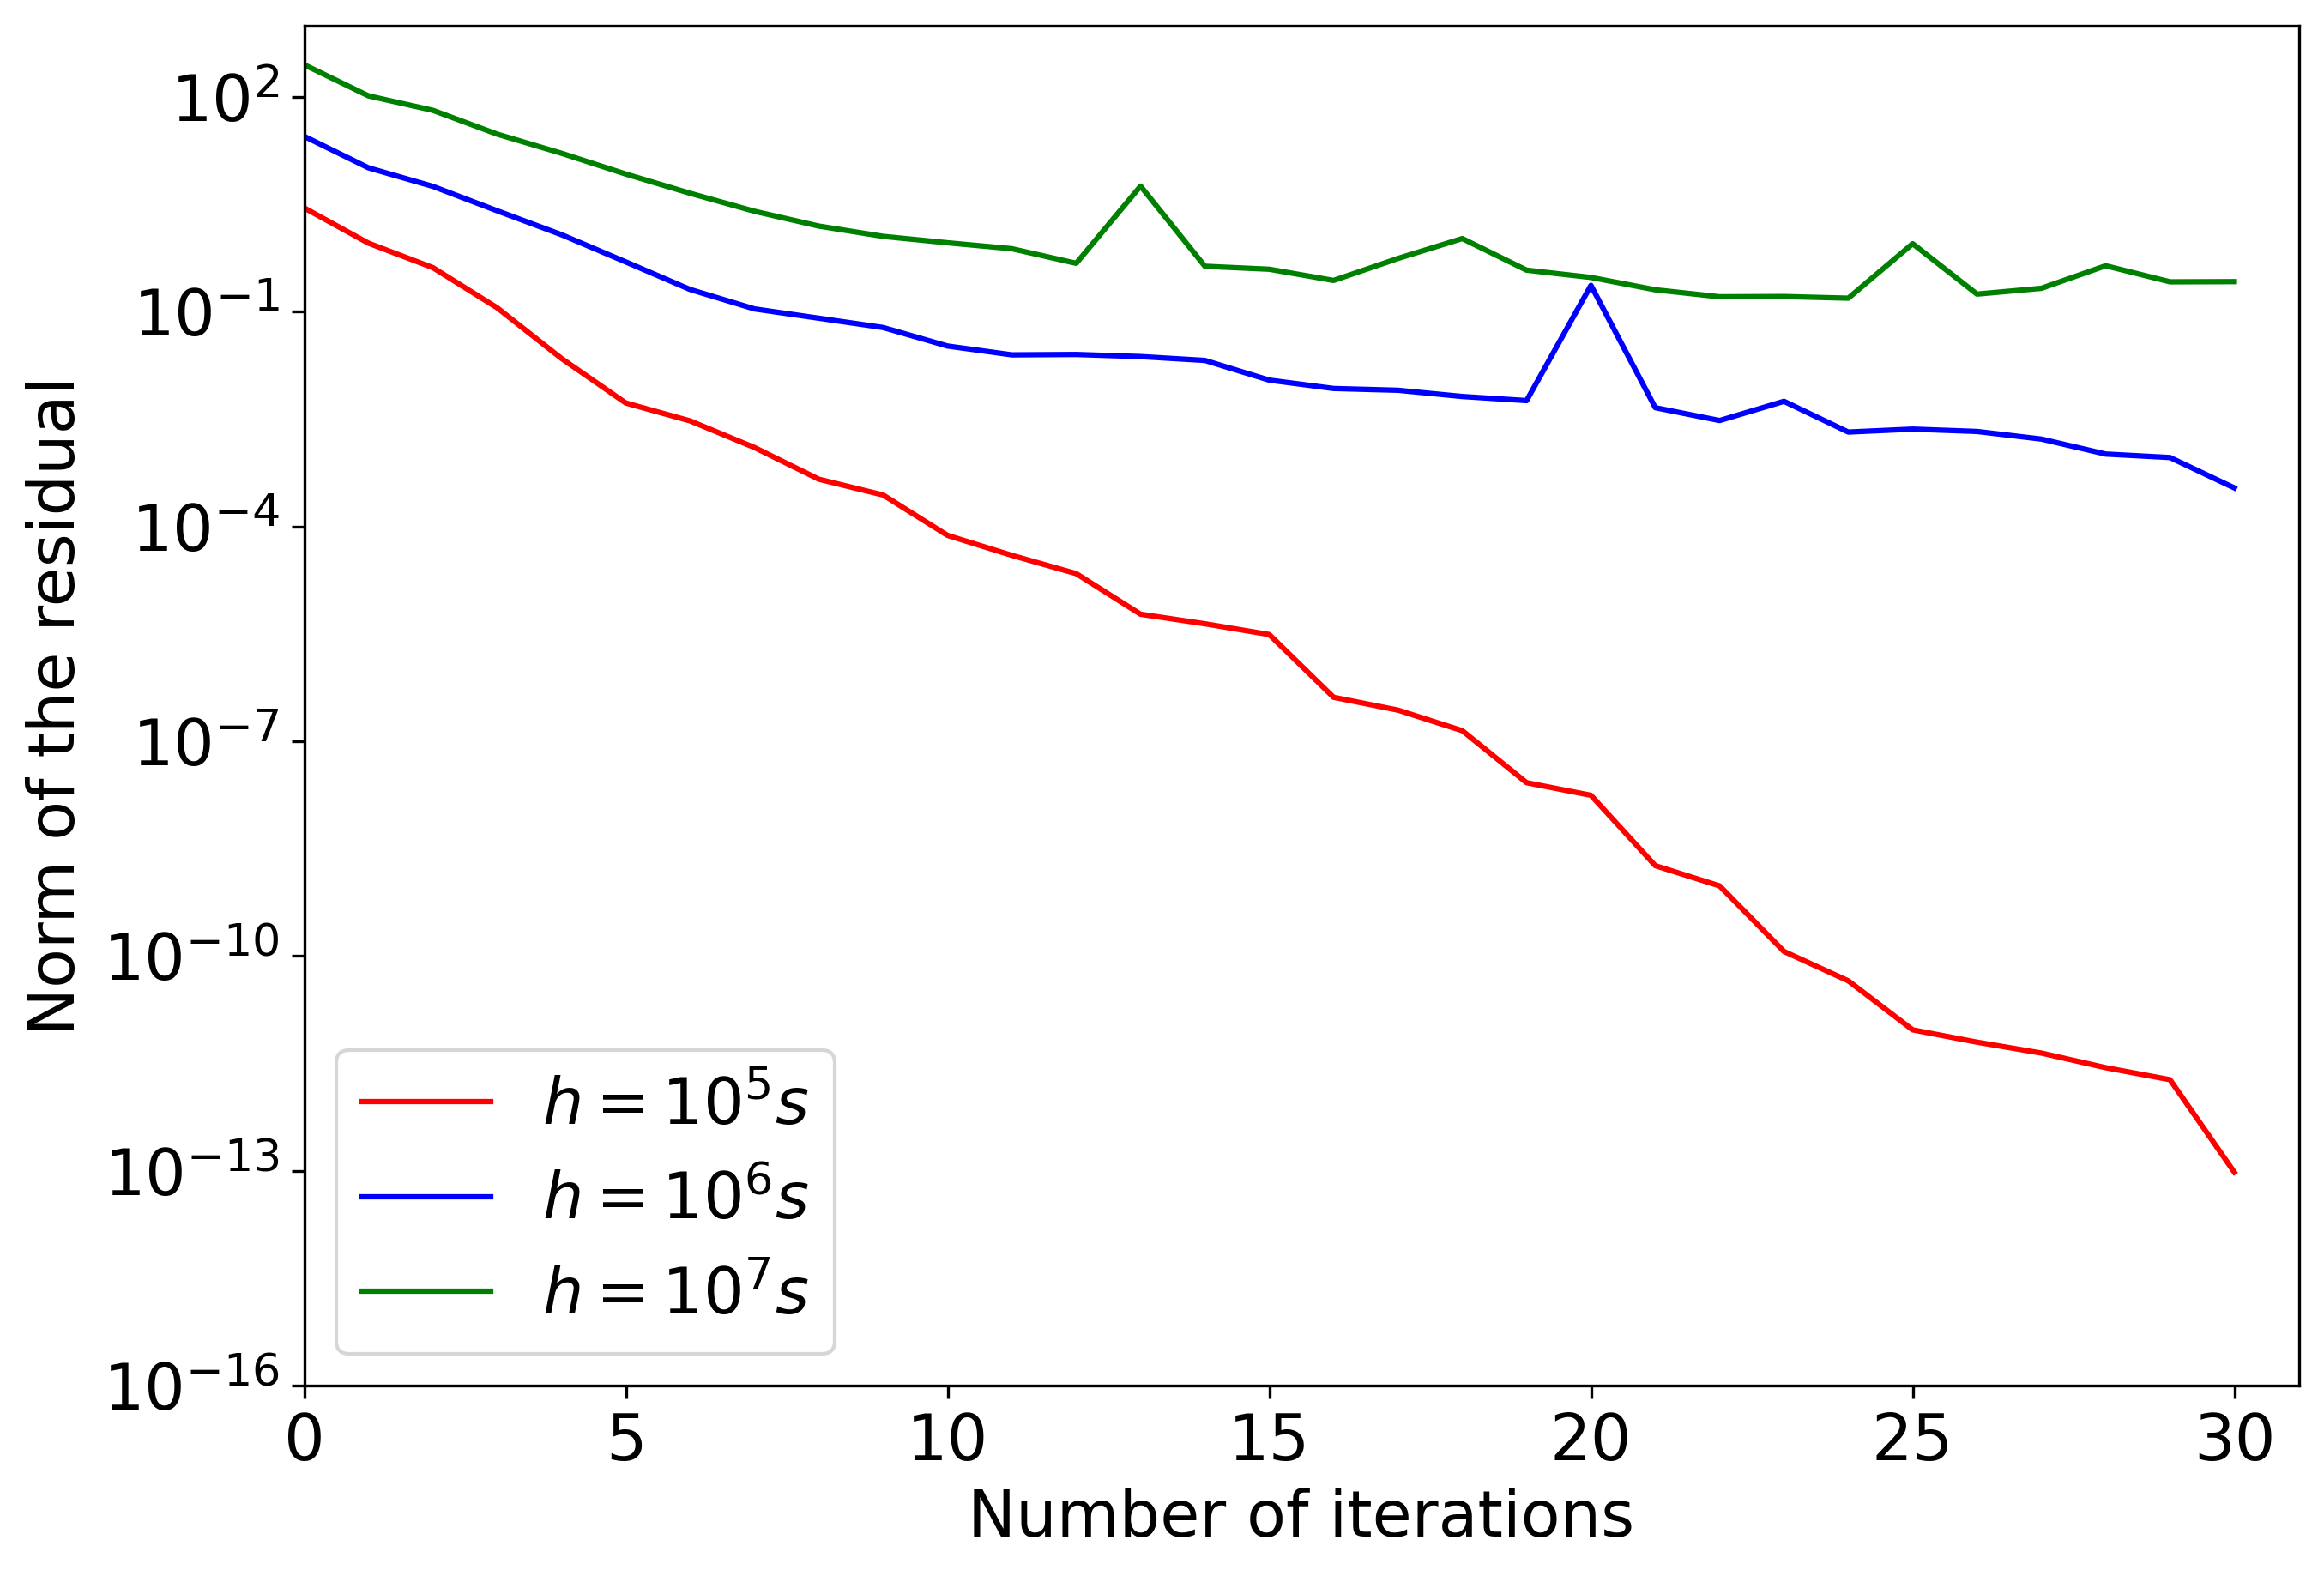
\includegraphics[width=1\textwidth]{images/NewtonIterationConvergence200Elements_DifferentDT_Broyden.png}
		\subcaption{Broyden iteration}
	\end{subfigure}
	\caption{Evaluation of the L2 norm of the residual $\phi(x_n)$ at each iteration of the Newton and Broyden methods for 200 fault elements}
	\label{fig:convergenceNewtonAndBroydenDifferentTimeSteps}
\end{figure}

It could be shown that the Newton iteration with the analytic Jacobian has excellent convergence properties for any domain sizes and large time step sizes. On the other hand, the alternative with a Broyden iteration, which approximates the Jacobian matrix along with the solution, converges only very slowly for large domains and large timesteps which is why this method is not suited to solve the problem. In practice, the  Newton iteration converges much faster because BDF schemes of higher order are used instead of the implicit Euler and the initial guess at the beginning of the iteration is obtained by extrapolating the previous solution vectors to the current simulation time. Usually, one Newton step is required to achieve the desired accuracy, which means two evaluations of the right-hand side function. \\

\subsection{Convergence issues with the compact DAE formulation}
The compact DAE formulation from \autoref{eq:DAE_compact_formulation_SEAS} shows a similar convergence behavior only during the aseismic slip. Whereas the method never diverges, the maximal achievable accuracy depends on the current time step size, in a way that for very small timesteps, the residual in the Newton iterations does not go below some large value. This bad convergence can be seen in \autoref{fig:convergenceIssuesCompactDAENewtonIterations}, which shows the infinity norm of the residual at each Newton step for different time step sizes. The largest instance, of the order $10^7$, is representative for the aseismic slip after the first earthquake and the other samples have been taken in the initial phase of the second earthquake, when the slip rate increases significantly and the timestep size decreases. \autoref{fig:convergenceIssuesCompactDAEMaxResidual_vs_dt} shows the maximum residual at the end of the Newton iteration in function of the current timestep size for all timesteps in the simulation. The locations of the samples in the first graph are highlighted by colored points. It can be clearly seen that a large residual norm inversely depends on the timestep size. \\ 
To obtain these results, the time integration itself has not been performed with the compact DAE formulation, since it obviously yields a poor accuracy, but rather with the 1st order ODE formulation using a classic adaptive RK4 scheme. At each timestep, the Newton iteration has been launched until the residual norm does not decrease anymore and the final result was discarded. Therefore, the solution vectors at the previous timesteps needed in the BDF method stem from the explicit RK4 time integration and thus slightly differ to the vectors in the time integration with the compact DAE formulation. To discuss the convergence, this difference is not significant, since the convergence issues arise in either case. \\

\begin{figure}[H]
	\centering
	\begin{subfigure}[t]{0.32\textwidth}
		\centering
		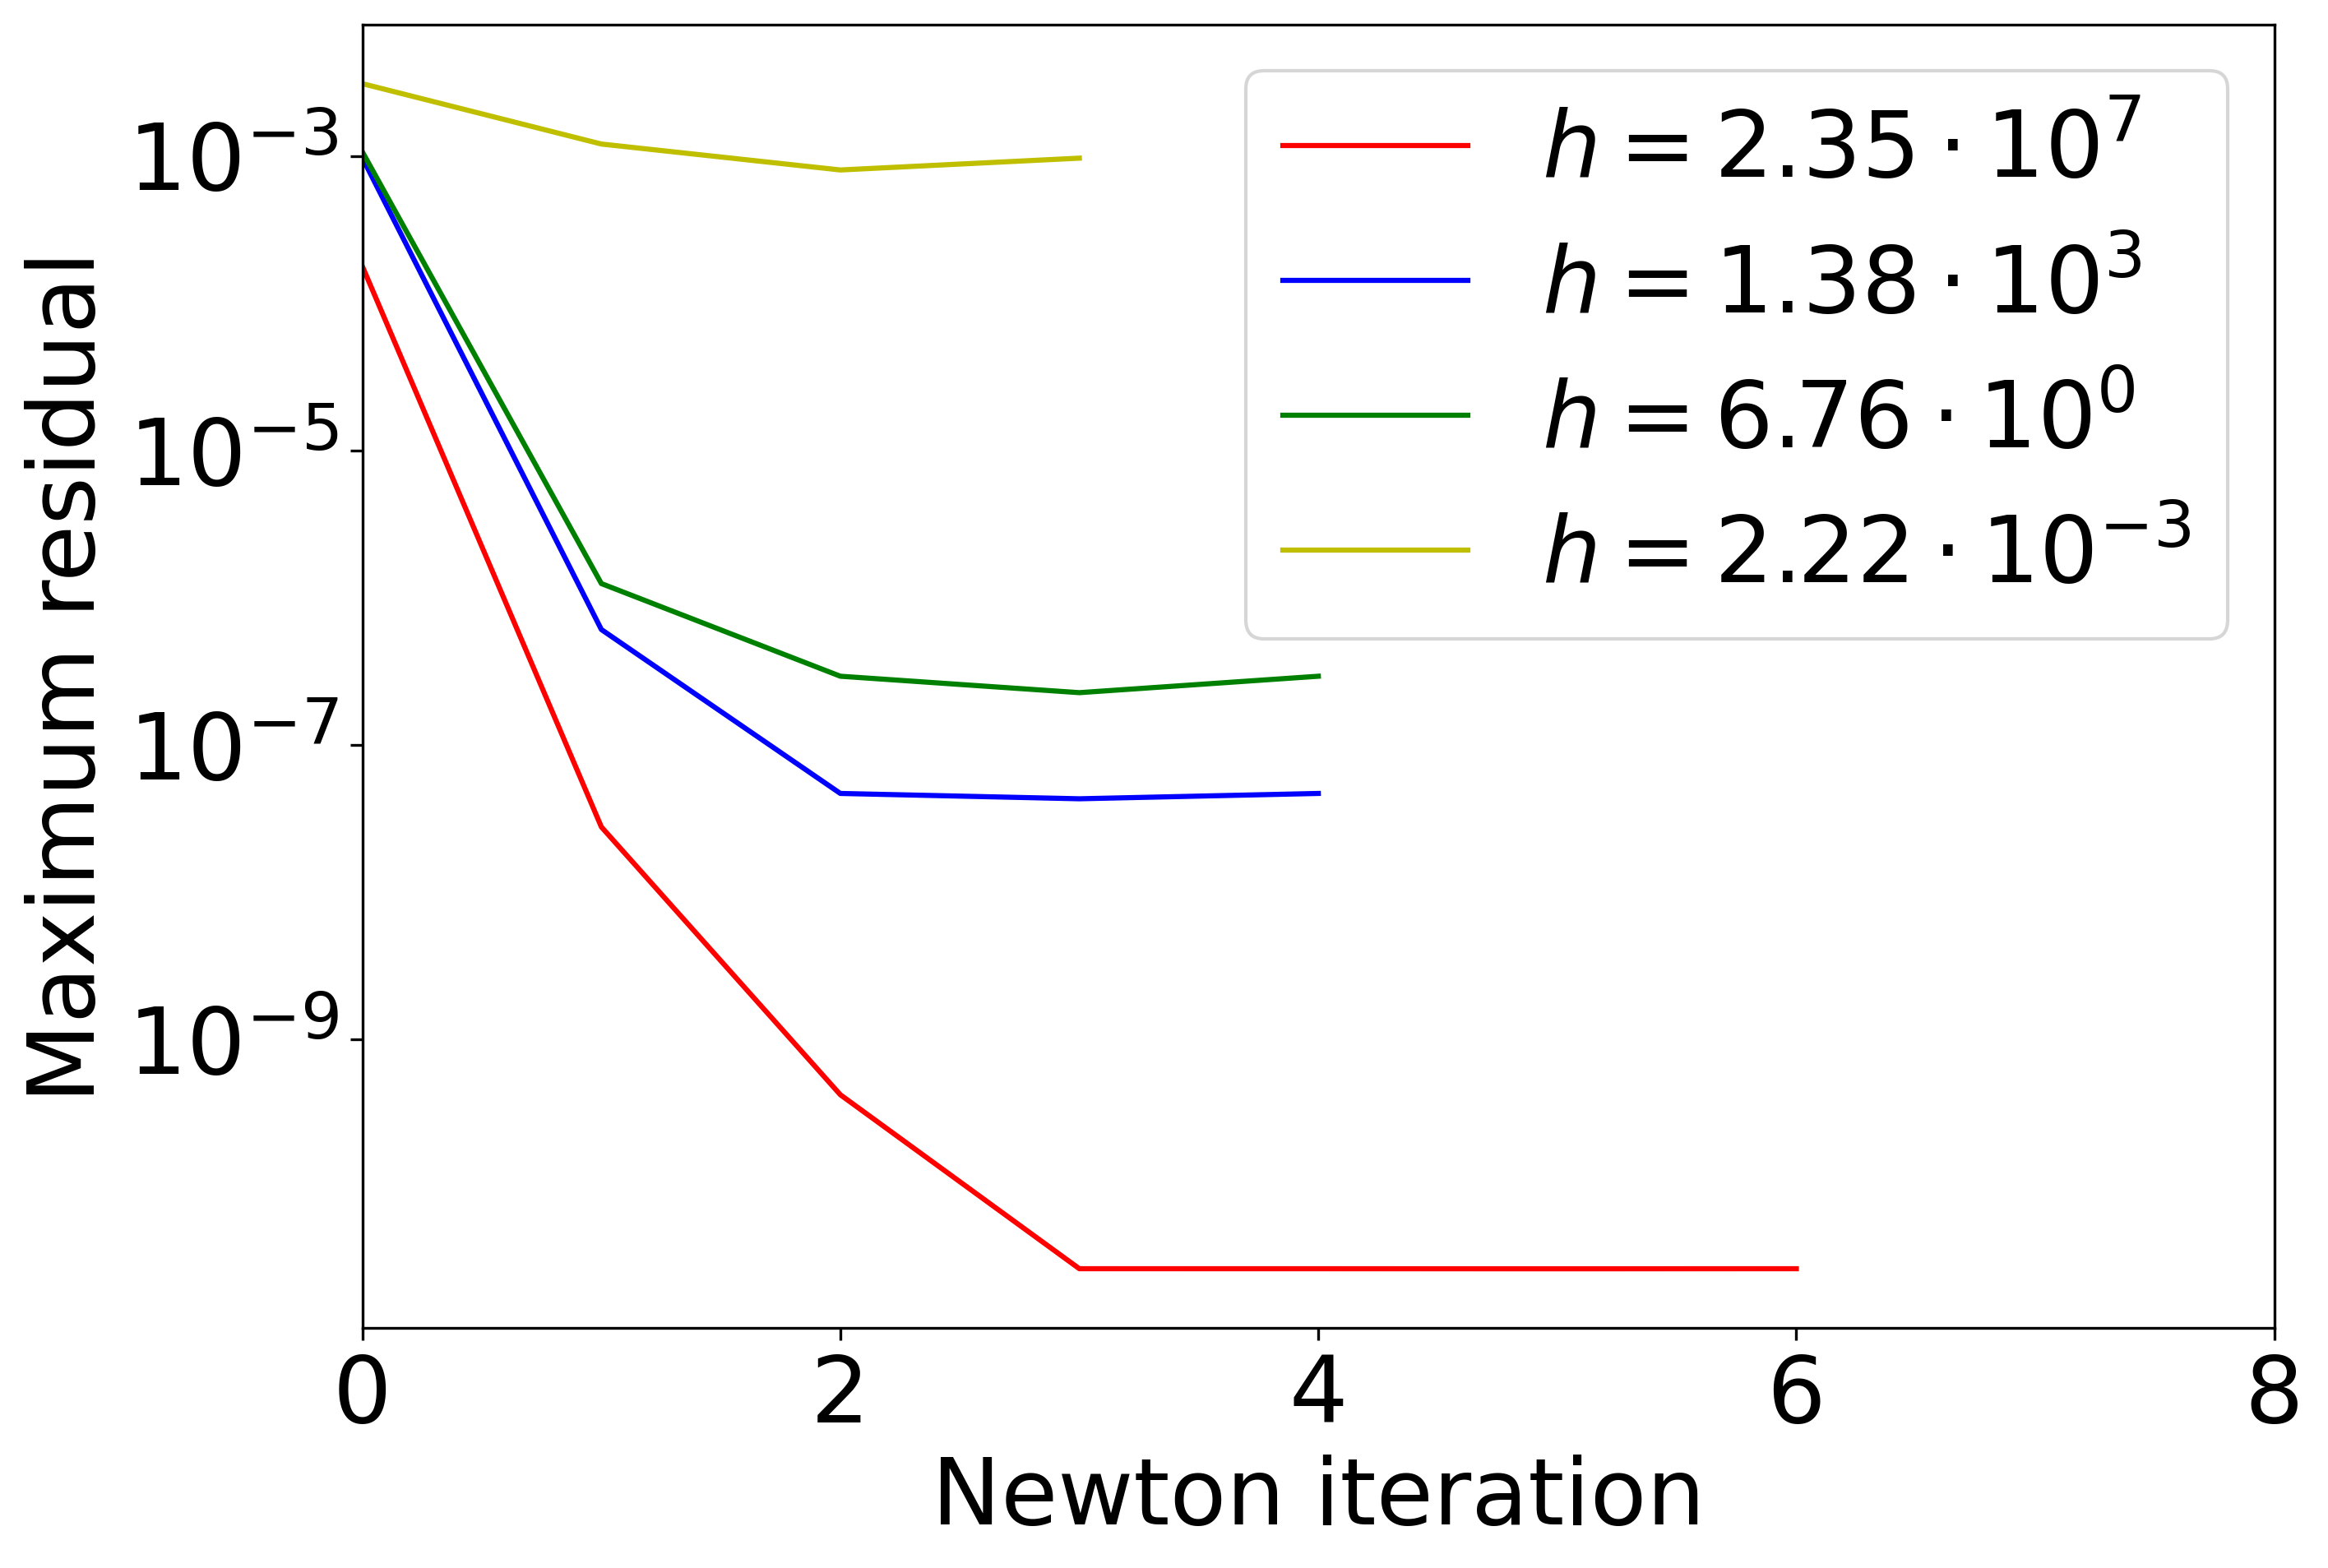
\includegraphics[width=0.9\textwidth]{images/TANDEMConvergenceAnalysisCompactDAENewton_Size5.png}
		\subcaption{$\infty$-norm of the residual in the Newton iterations at different time step sizes}
		\label{fig:convergenceIssuesCompactDAENewtonIterations}
\end{subfigure}
	\begin{subfigure}[t]{0.32\textwidth}
		\centering
		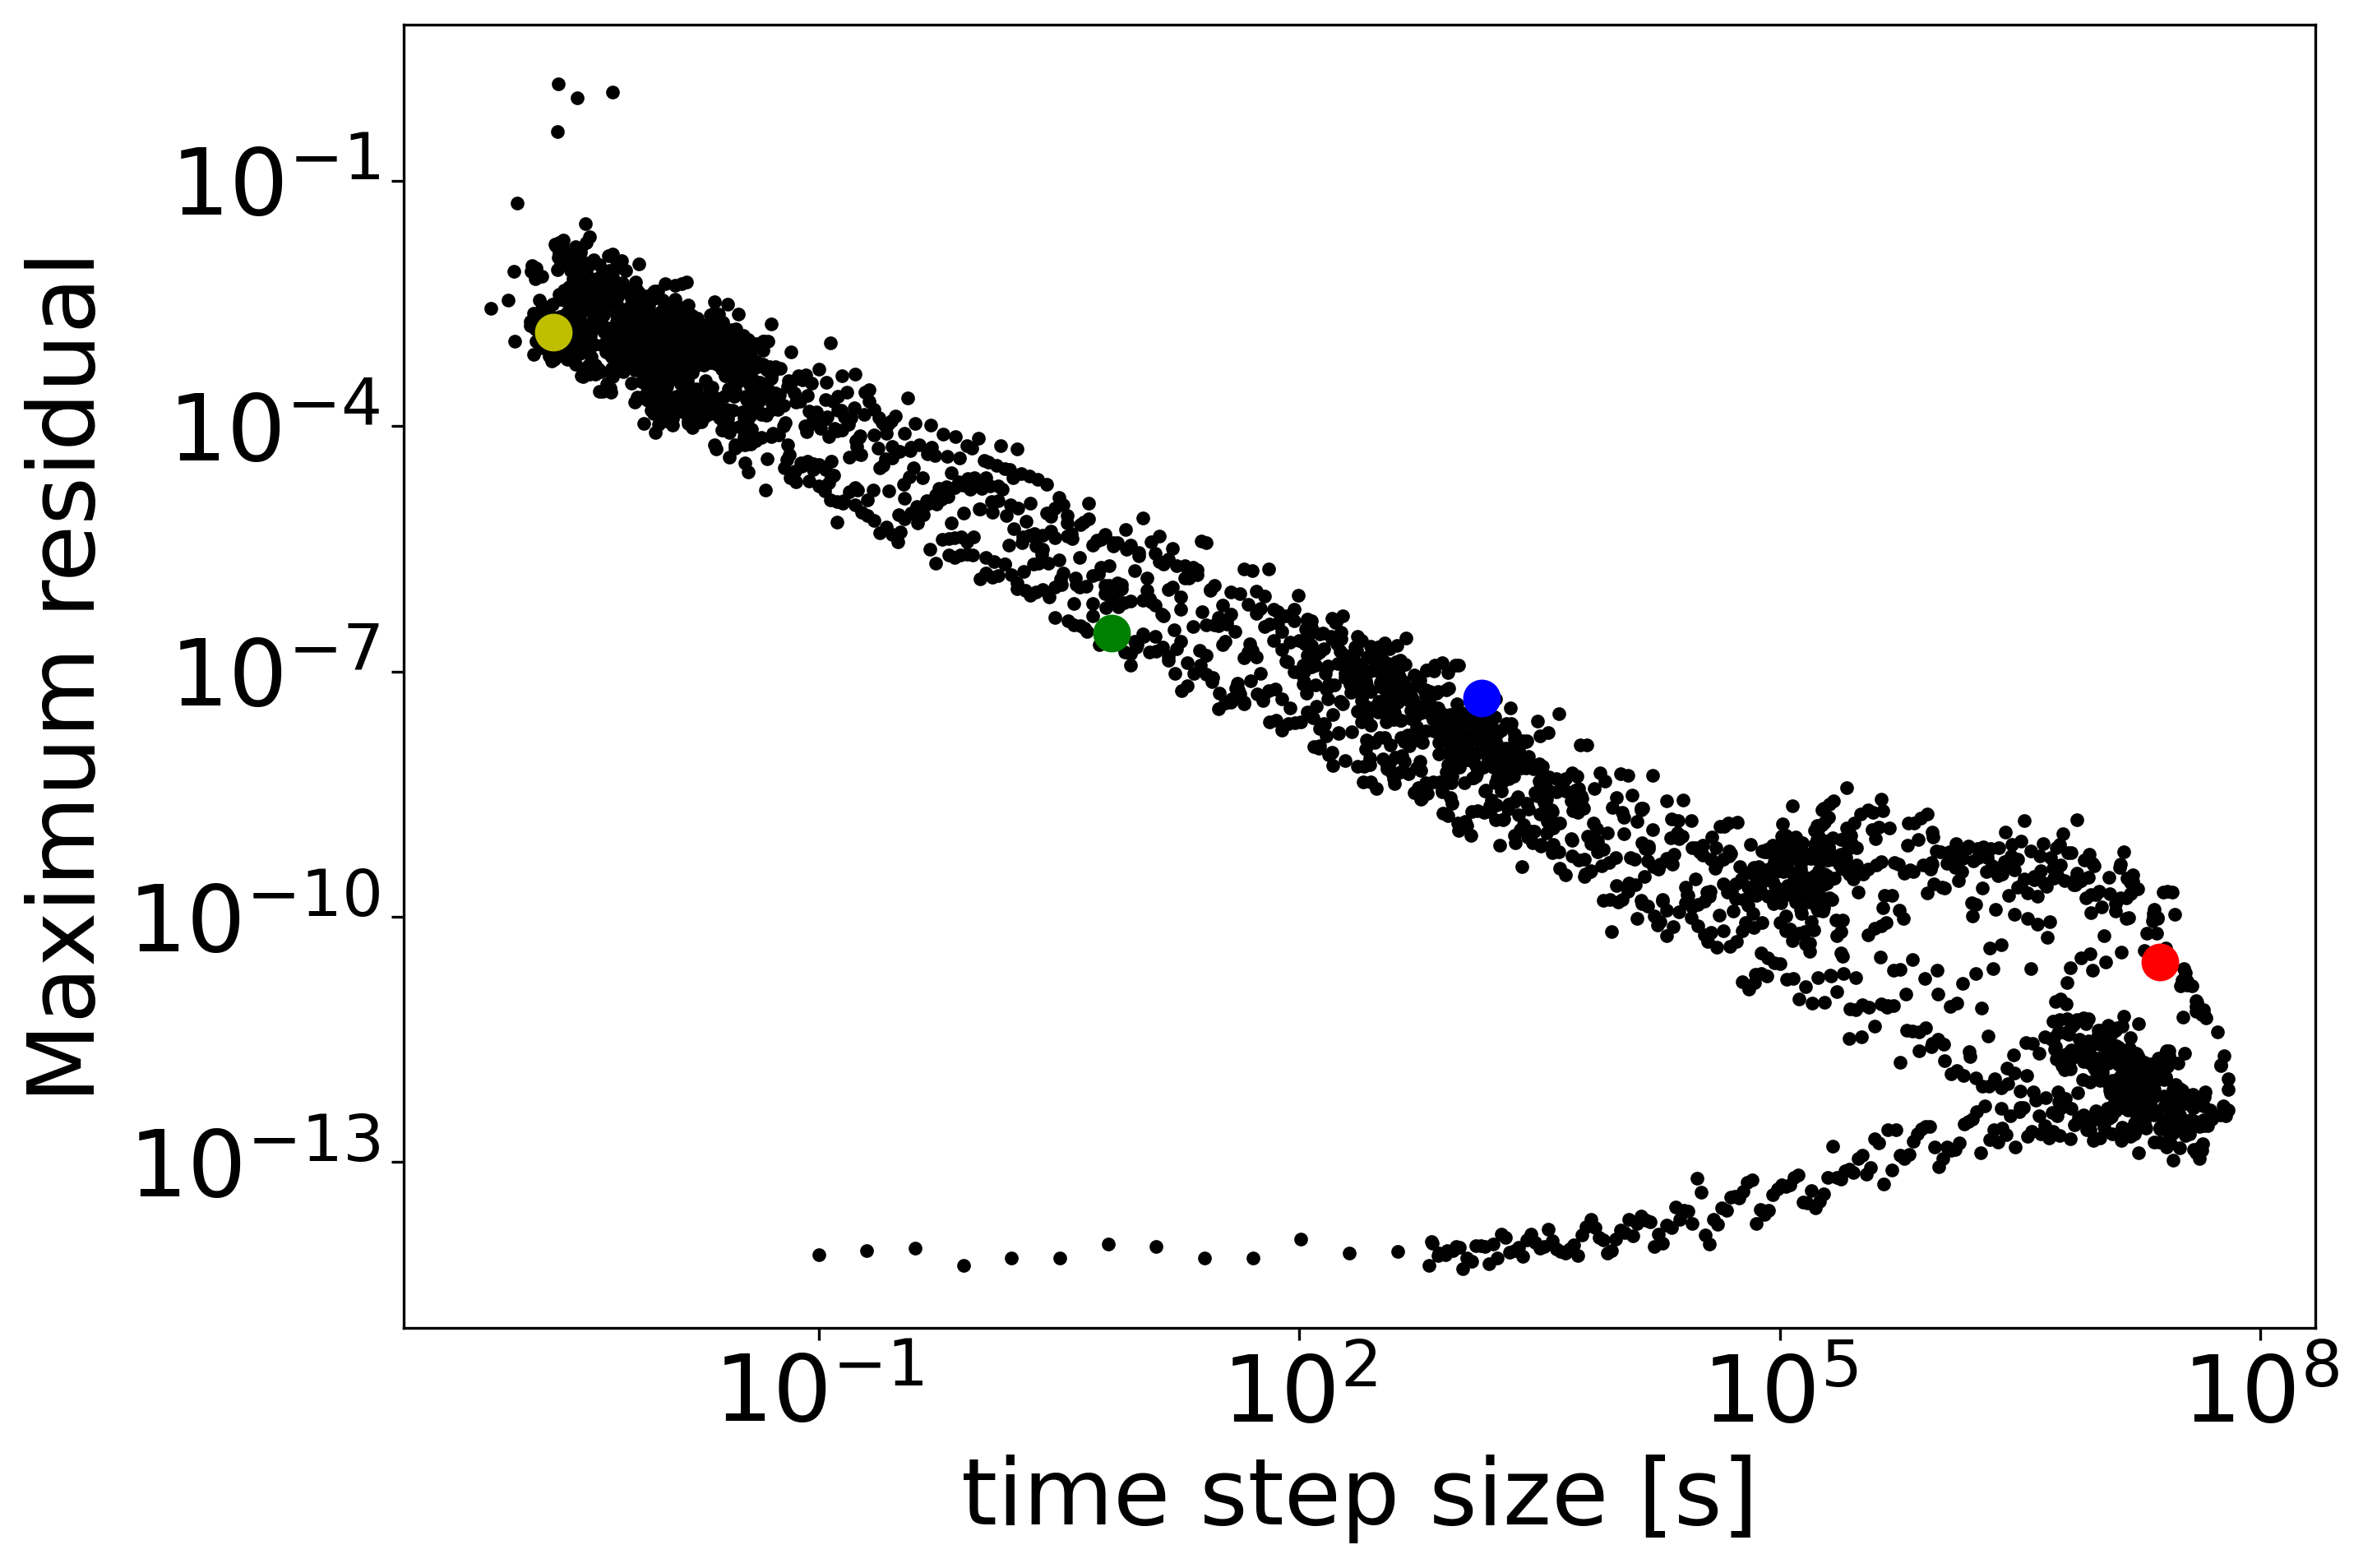
\includegraphics[width=1\textwidth]{images/TANDEMConvergenceAnalysisCompactDAEMaxResidual_Size5.png}
		\subcaption{Minimum achievable residual norms in function of the timestep size}
		\label{fig:convergenceIssuesCompactDAEMaxResidual_vs_dt}
	\end{subfigure}
	\begin{subfigure}[t]{0.32\textwidth}
		\centering
		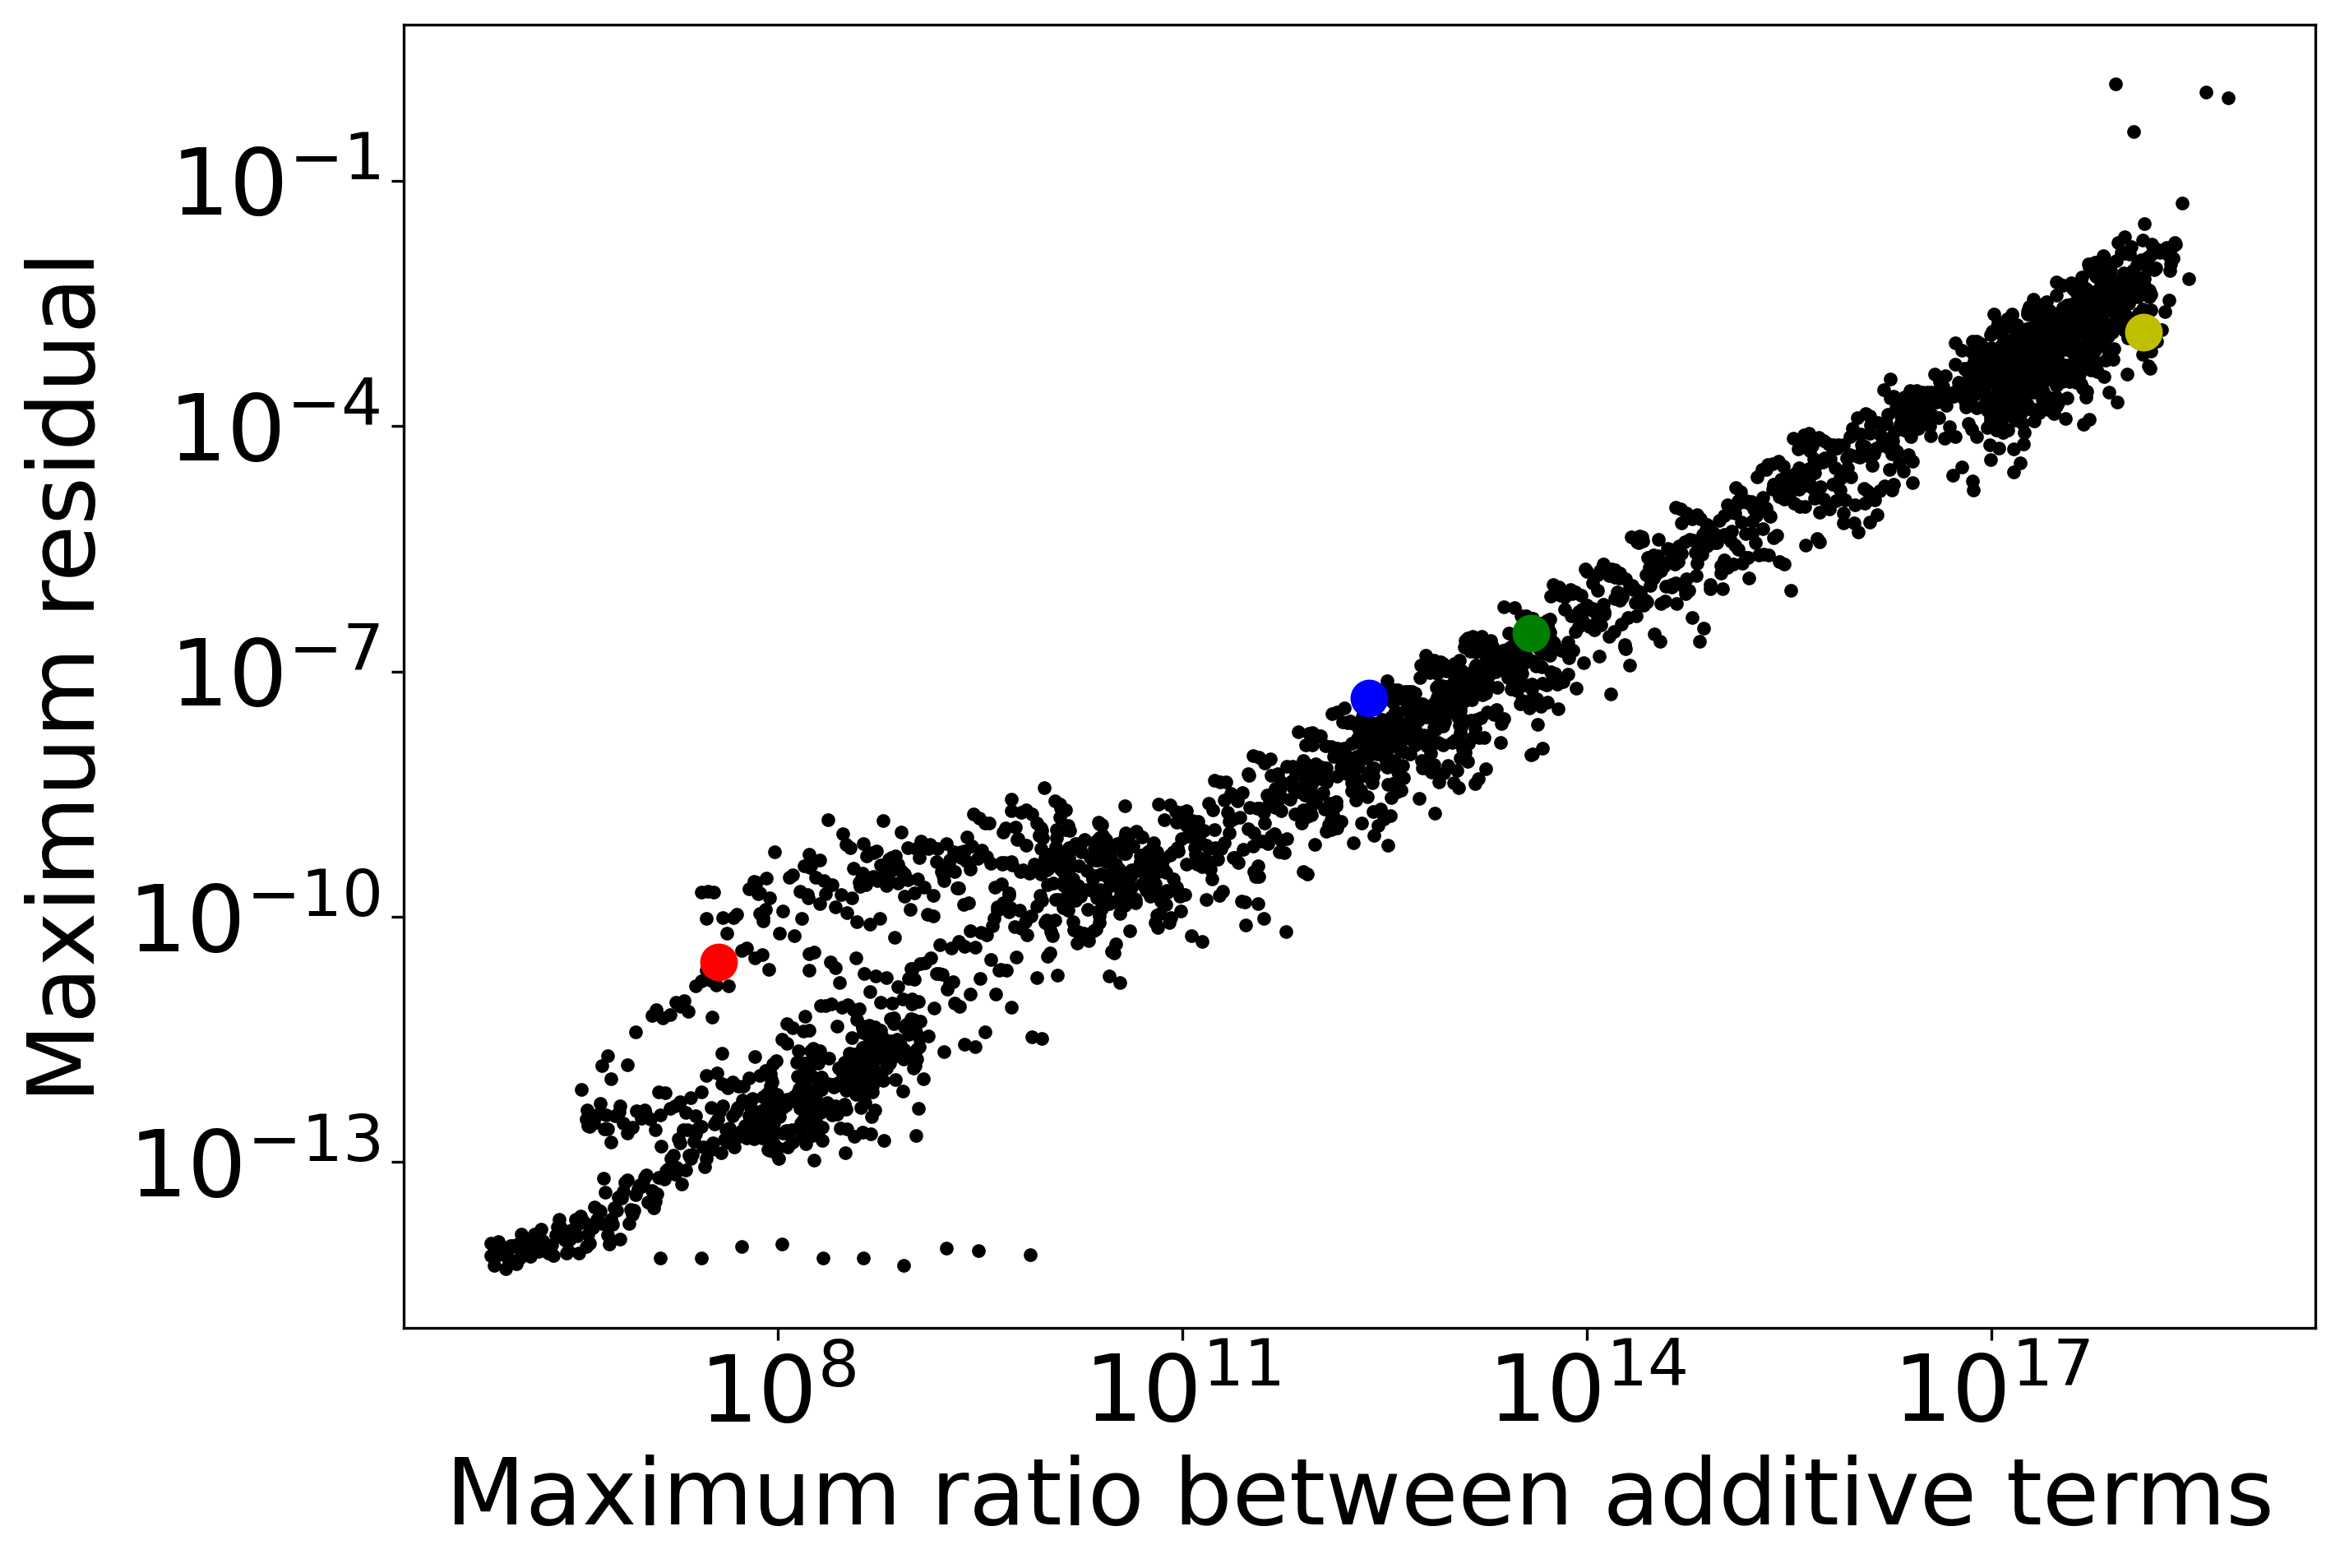
\includegraphics[width=1\textwidth]{images/TANDEMConvergenceAnalysisCompactDAERatioInAddition_Size5.png}
		\subcaption{Minimum achievable residual norms in function of the maximal ratio between the additive terms in the Jacobian matrix}
		\label{fig:convergenceIssuesCompactDAEMaxResidual_vs_ratio}
	\end{subfigure}
	\caption{Convergence properties of the compact DAE formulation with the 4th order BDF method on a small domain with 5 fault elements}
\end{figure}

The reason for this poor convergence can be found in the definition of the Jacobian matrix of the compact DAE formulation in \autoref{eq:Jacobian_compact_DAE}. As a quick remainder, the Jacobian matrix in the Newton iteration is obtained by $\mathbf{J} = \mathbf{F}_x + \sigma \mathbf{F}_{\dot{x}}$, where the shift $\sigma$ depends on the order $k$ of the BDF scheme and on the timestep sizes in the $k$ previous timesteps. The upper left block in the Jacobian is thus the sum of $\sigma\pdv{f}{V}$ and $\pdv{f}{S}$. The first partial derivative is of the magnitude $10^9$ in the aseismic slip and reaches values up to the order $10^{15}$ in an earthquake. On the other hand, the second summand takes values between $10^0$ and $10^2$. Since the former is a diagonal matrix, the sum only affects the diagonal elements. The timestep does not change by a lot between two time iterations, it can be assumed that they are of the same order of magnitude. The shift $\sigma$ is then of the order $\sigma = \Theta\left(h_n^{-1}\right)$, where $h_n$ is current timestep size. In the aseismic slip, $\sigma$ is thus of the order $10^{-7}$ and can go as high as $10^3$ during an earthquake. In the worst case, two terms of orders $10^{18}$ and $10^0$ have to be summed up, which cannot be represented anymore by a double precision floating point variable. The partial derivative $\pdv{f}{S}$ is therefore neglected in the Jacobian matrix during an earthquake and the friction law cannot be solved accurately anymore.
\autoref{fig:convergenceIssuesCompactDAEMaxResidual_vs_ratio} shows the maximum residual at the end of the Newton iteration in function of the ratio $\sigma\pdv{f}{V} / \pdv{f}{S}$ between the two problematic summands. As the ratio approaches and surpasses the machine precision of approximately $10^{16}$, the minimal achievable residual norm also increases. As a matter of fact, the bad accuracy only appears in the residual components in $S$, for which the problematic summation occurs, whereas the residual components in $\psi$ remain at very good values below $10^{-12}$ throughout the simulation.
\\
In the last two graphs, a band with high accuracy and low timestep size appears at the bottom. These points correspond to the initial phase of the simulation, which is always launched in the aseismic slip phase with $h_0=0.1s$. Since the solution vector contains the initial value in these points, the Newton iteration converges directly with a high precision. \\
This issue occurs only with the compact DAE formulation, because the Jacobian matrices of the ODE formulations do not require any summations and in the extended DAE formulation, the two problematic terms $\pdv{f}{V}$ and $\pdv{f}{S}$ are located in different submatrices of $\mathbf{F}_{\dot{x}}$ and $\mathbf{F}_x$ and are thus never added to each other. \autoref{fig:convergenceIssuesExtendedDAEMaxResidual_vs_dt} shows the same dependency as in \autoref{fig:convergenceIssuesCompactDAEMaxResidual_vs_dt} for the extended DAE formulation. The norm of the residual at the end of the Newton iteration here does not depend on the timestep size and it varies between $10^{-12}$ and $10^{-15}$ throughout the simulation. Since both the slip and the state variable are of the order of $10^0$, the achieved tolerance is excellent and close to machine precision. However, it seems that the best accuracy is only reached for large timesteps, whereas for very small timesteps, the Newton iteration only reached the "not the best but still very good" - accuracy of $10^{-12}$. In the definition of the Jacobian matrix for the extended DAE formulation in \autoref{eq:Jacobian_Newton_Iteration_extended_DAE}, there still is an addition between the shift $\sigma$ ($\sigma=1/h$ in the referred equation because it is related to the implicit Euler method) and the term $\pdv{g}{\psi}$. Since this last term is always of the order $10^{-7}$, the difference between the summands is not as extreme as for the compact formulation, but still noticeable for small time steps, where $\sigma \approx 10^3$. Looking at \autoref{fig:convergenceIssuesExtendedDAEMaxResidual_vs_dt_onlyPSI}, the components of the residual vector relative to $\psi$ increase if the timestep size decreases. This is the same behavior as previously, but on a much lower magnitude. Only in the earthquake phase, when timesteps below $0.1s$ are encountered, the residual in $\psi$ exceed the maximal precision $10^{-15}$ of the friction law and impacts the overall accuracy. 

\begin{figure}[H]
	\centering
	\begin{subfigure}[t]{0.45\textwidth}
	\centering
		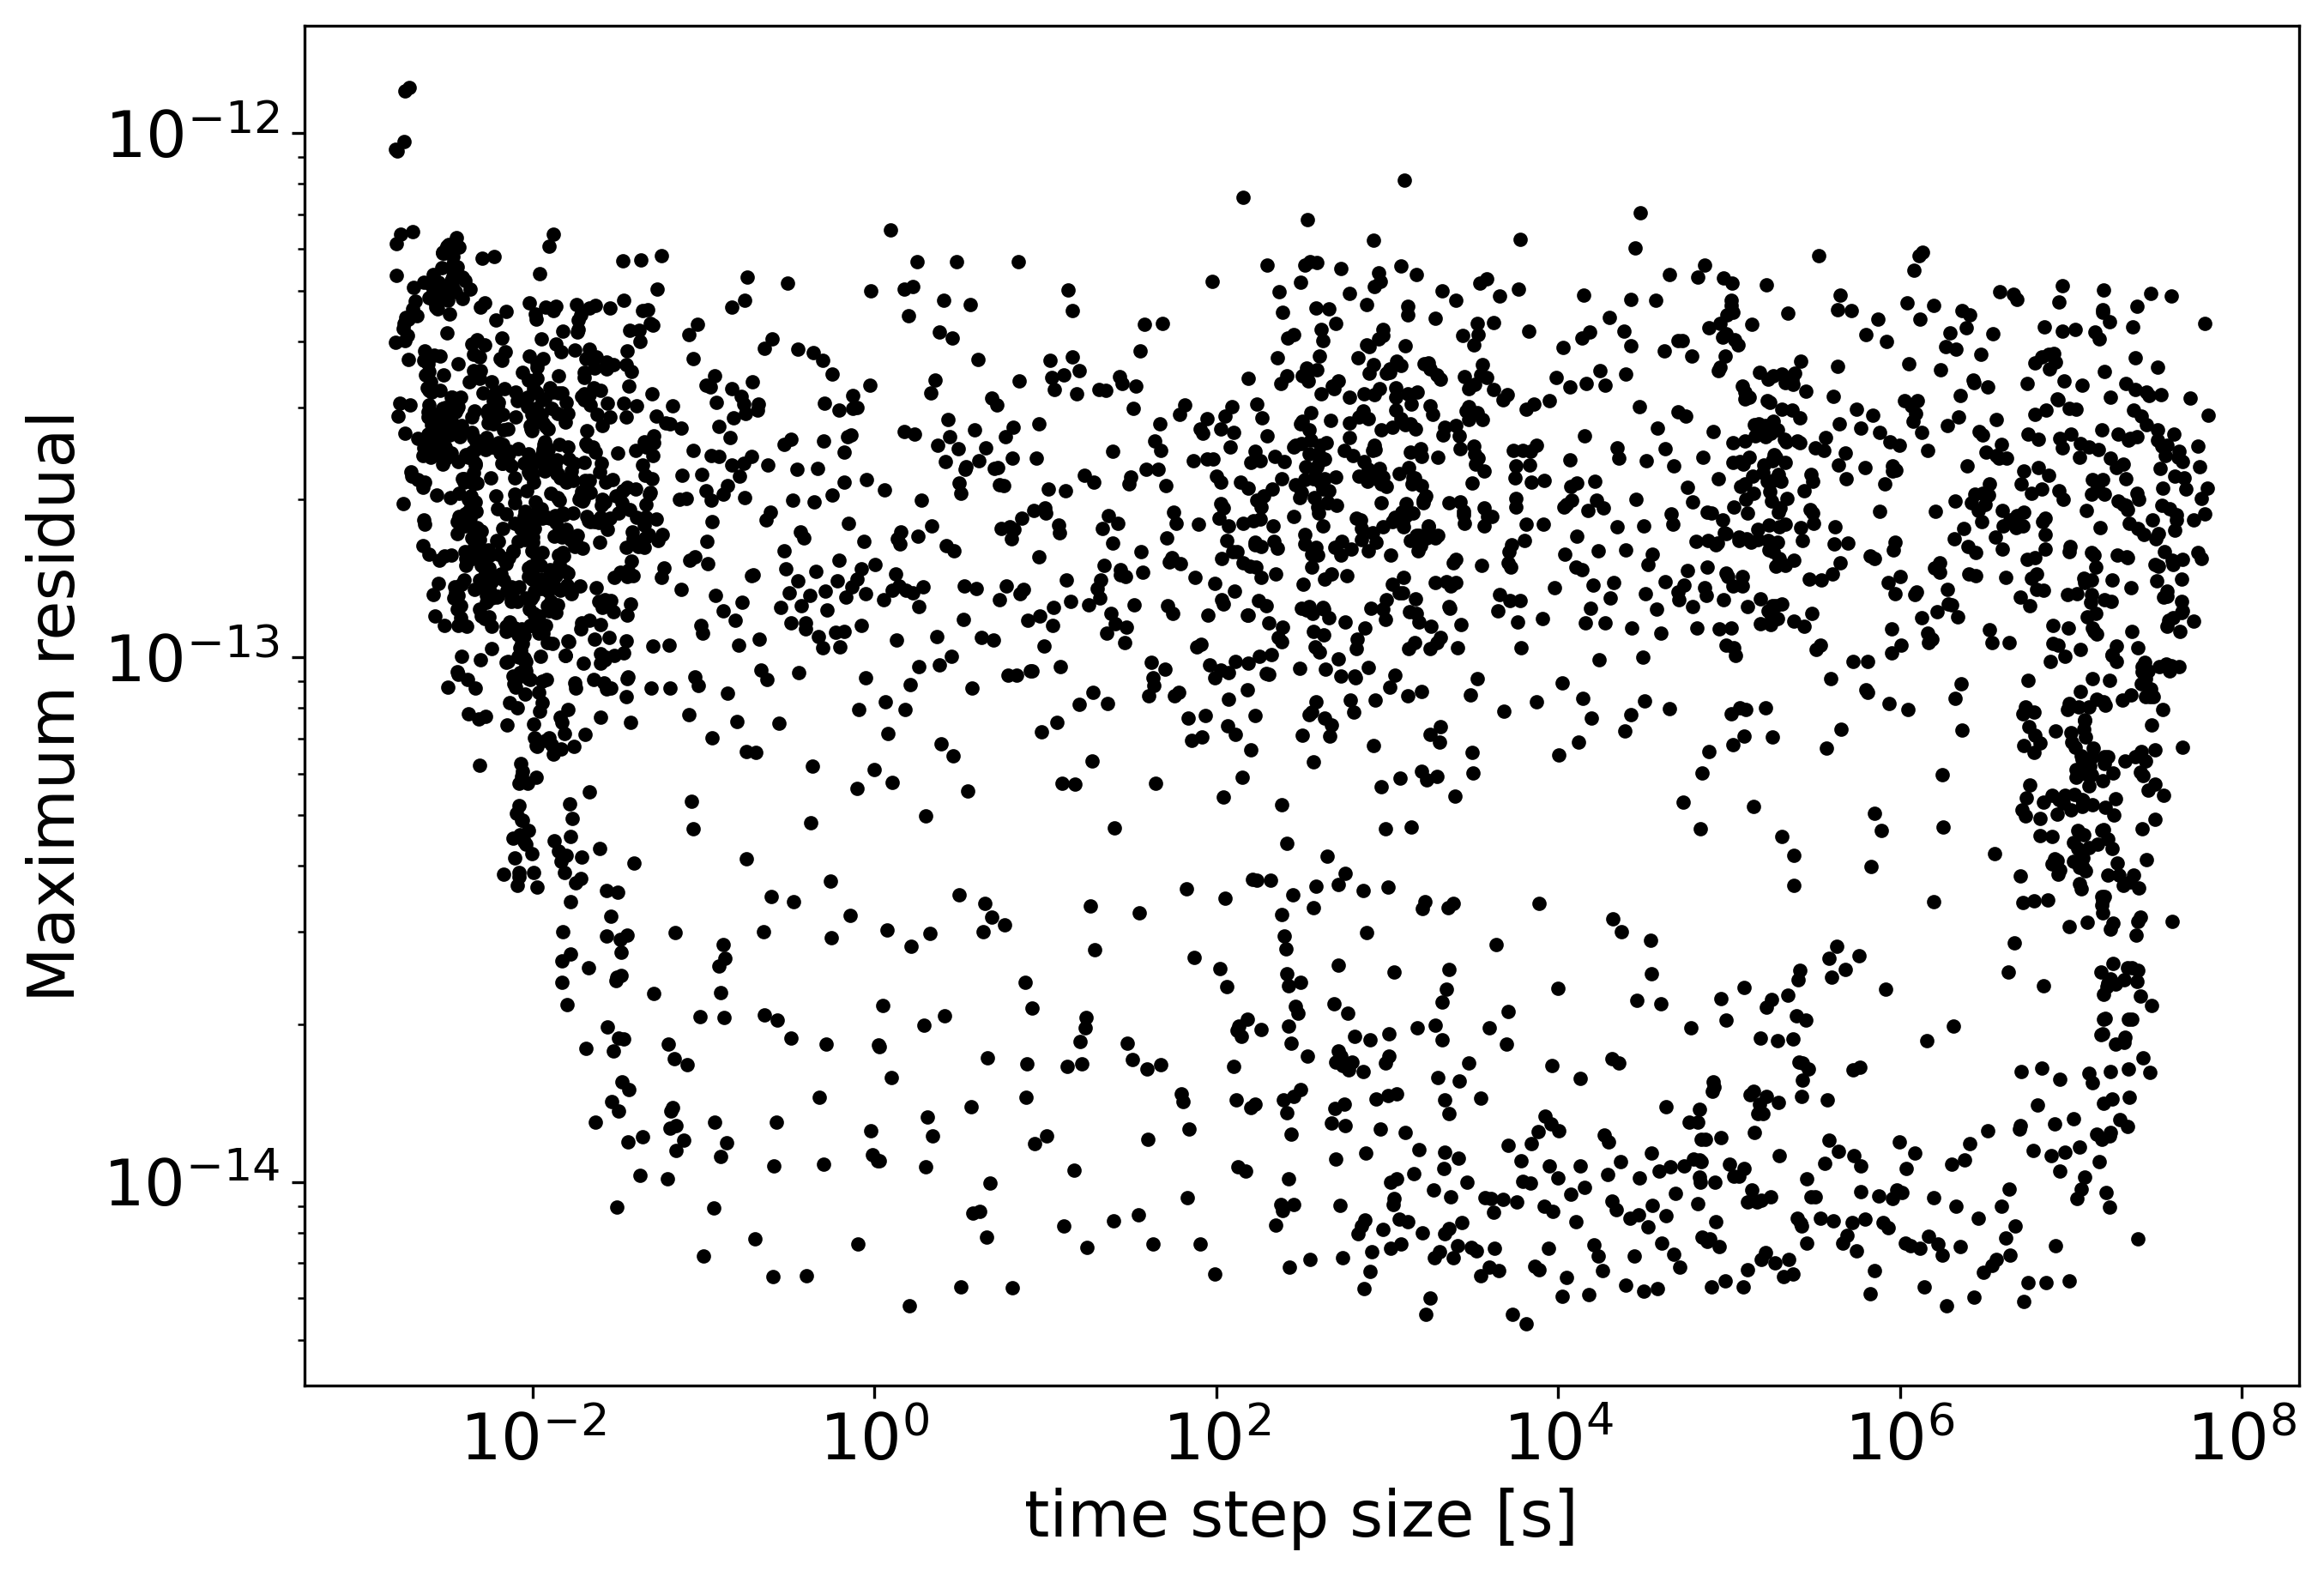
\includegraphics[width=1\textwidth]{images/TANDEMConvergenceAnalysisExtendedDAEMaxResidual_Size5.png}
		\caption{Residual of all components}
		\label{fig:convergenceIssuesExtendedDAEMaxResidual_vs_dt}
	\end{subfigure} 
	\begin{subfigure}[t]{0.45\textwidth}
		\centering
		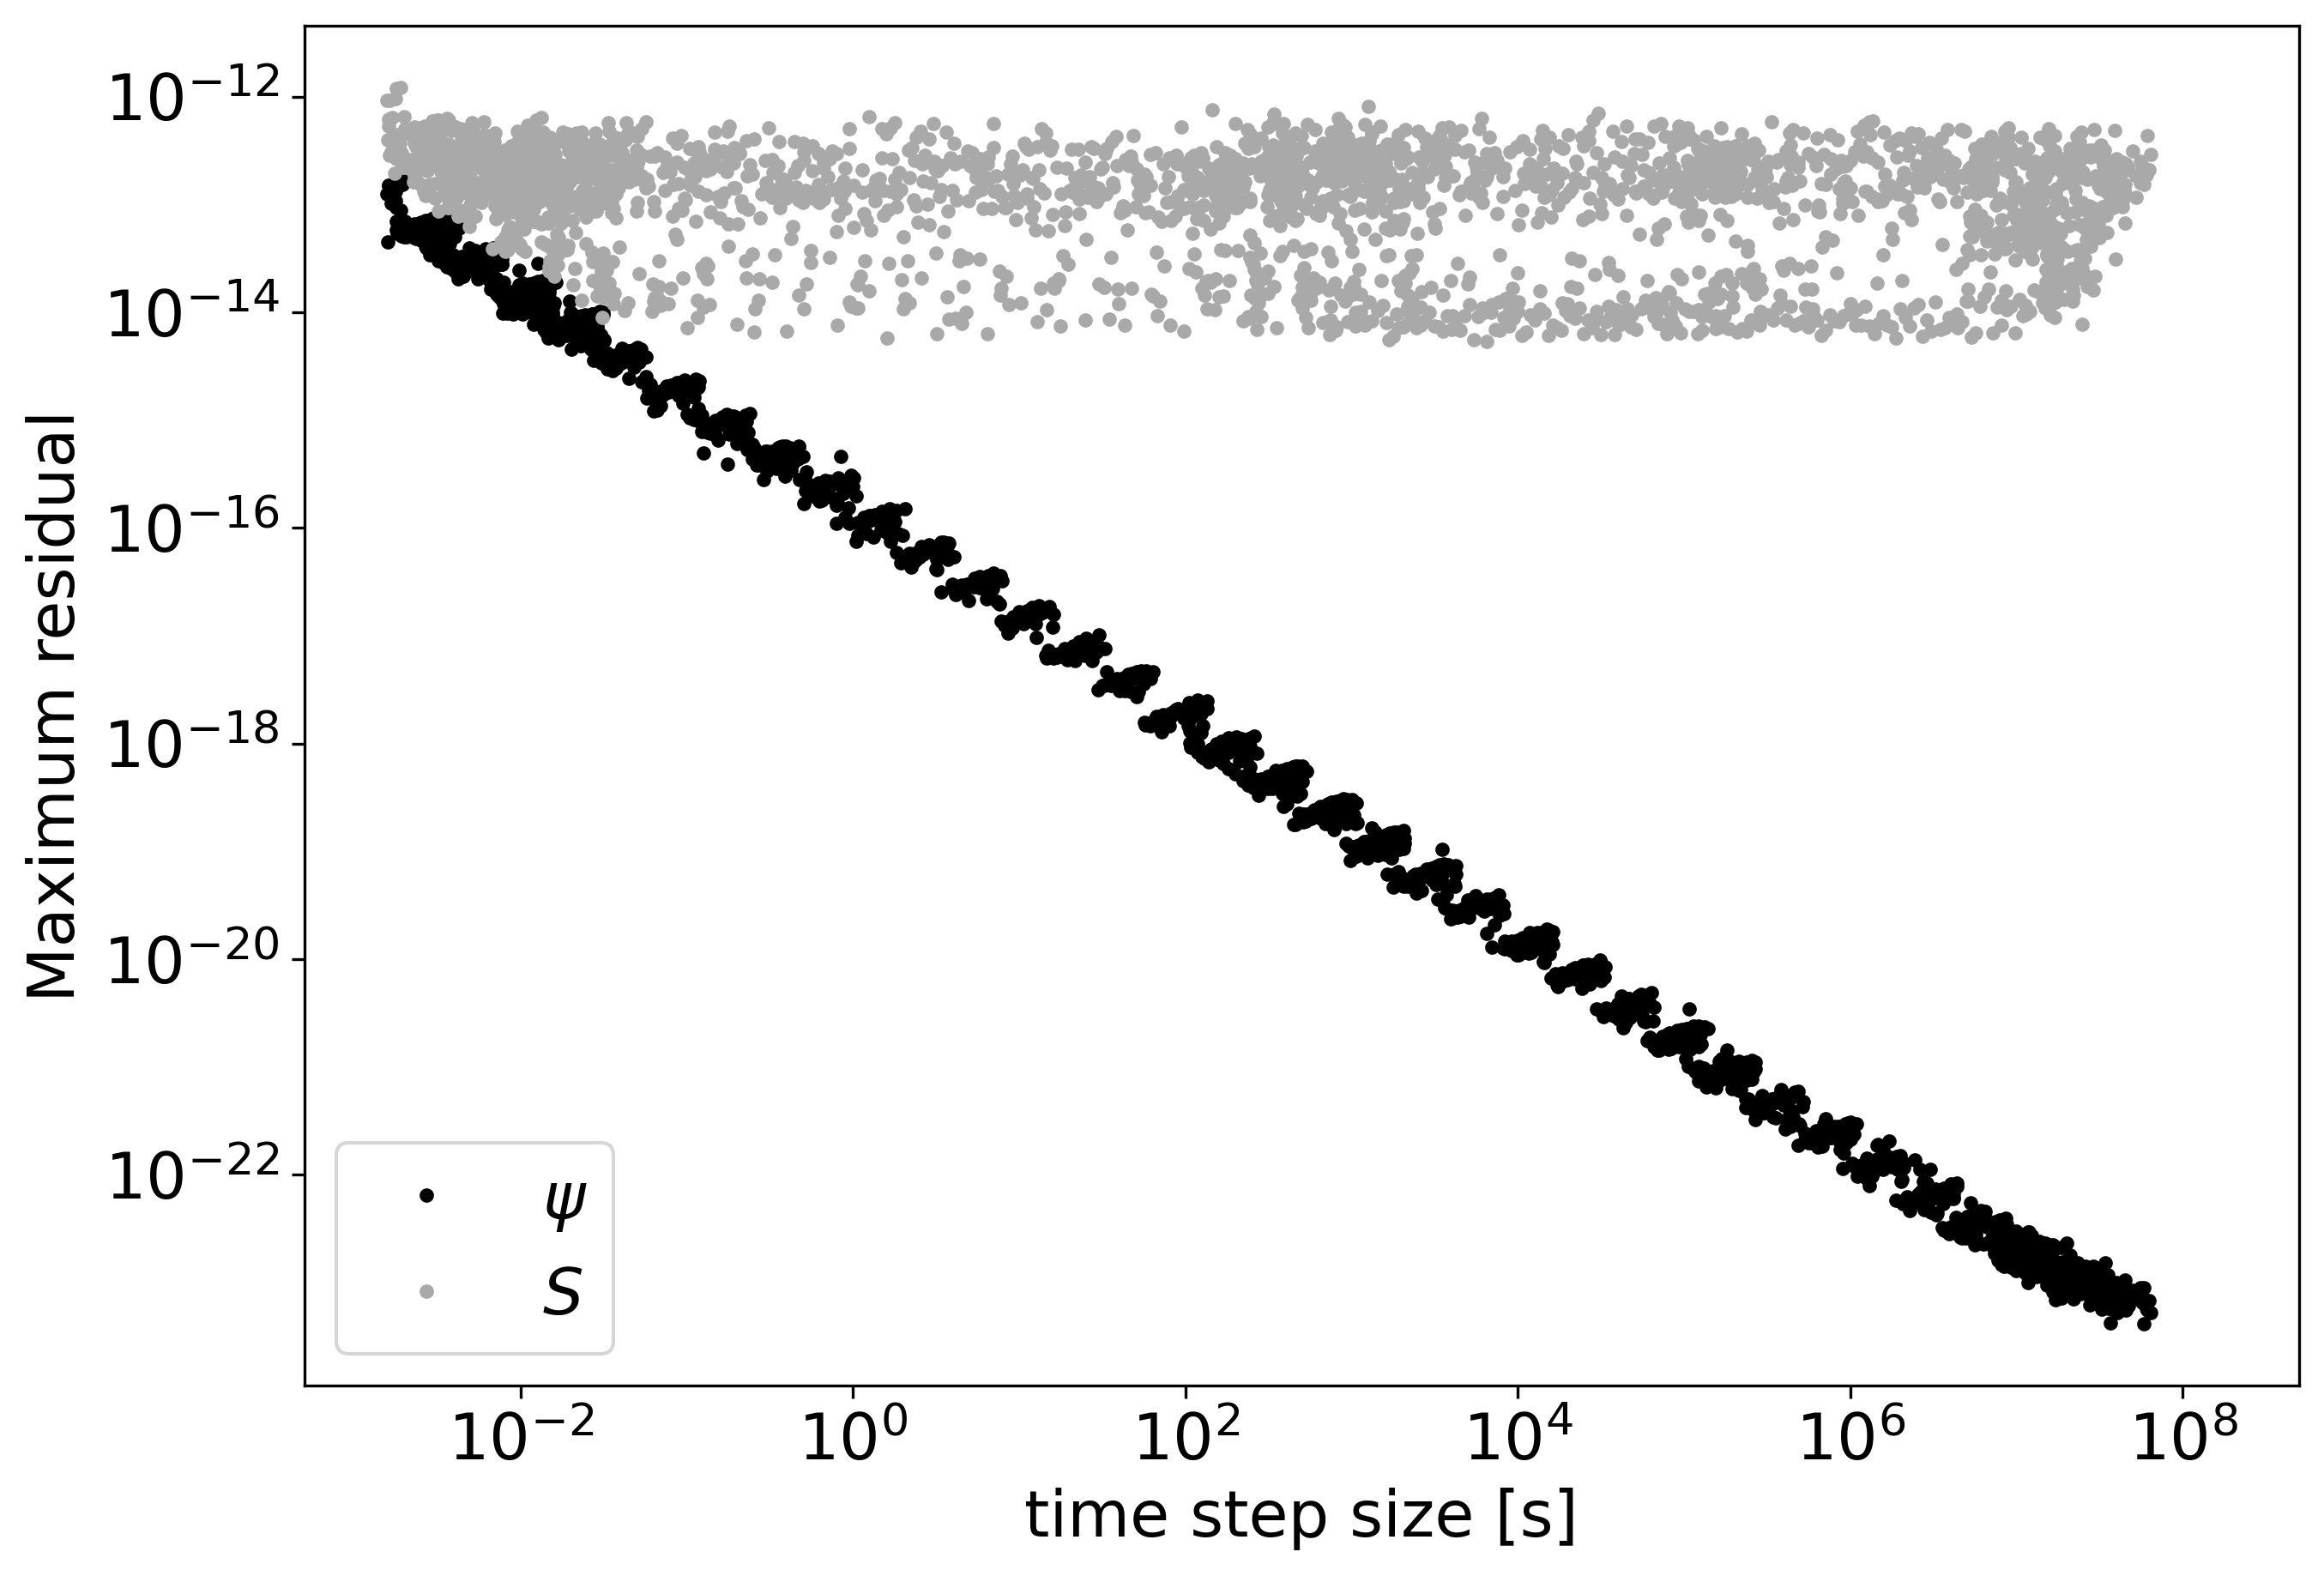
\includegraphics[width=1\textwidth]{images/TANDEMConvergenceAnalysisExtendedDAEMaxResidual_Size5_onlyPSI.png}
		\caption{Residual of the individual components $\psi$ and $S$}
		\label{fig:convergenceIssuesExtendedDAEMaxResidual_vs_dt_onlyPSI}
	\end{subfigure} 
	\caption{Minimum achievable residual norms in function of the timestep size for the extended DAE formulation with the 4th order BDF method on a small domain with 5 fault elements}
\end{figure}


In conclusion, the compact DAE formulation fails for the earthquake and can only be applied in the aseismic slip phase. Since the accuracy decreases along with the timestep size, the usual strategy to restart a step with a smaller timestep size if the nonlinear did not converge only leads to an even worse accuracy and is unsuitable. For this limited purpose, it still offers advantages over other methods which will be discussed in a further section.

\subsection{Stopping criterion}
The Newton iteration should be stopped when the norm of the residual reaches some tolerance value or if the last Newton step could not decrease the norm further, as it happened for the compact DAE formulation. In this latter case, the Newton iteration is not rejected, because the standard PETSc approach to reduce the timestep size does not allow a better convergence. Instead, a warning is printed to the terminal to notify the user that the Newton iteration could not reach the requested accuracy. In case a NaN value is encountered in the solution vector, or if the residual norm is larger then the initial norm, divergence is declared and an order to PETSc is ordered to restart the current timestep with a smaller timestep size. \\
It makes sense to prescribe different tolerances for the components of the residual in $S$, $\psi$, $V$ or $f$ as for the time integration, since their magnitudes greatly differ. To ensure comparability with explicit methods, the friction law is always solved up to the maximum precision $\varepsilon_{max}$. The other tolerances are defined in a way that the local truncation errors in $\varepsilon^S$, $\varepsilon^\psi$ and $\varepsilon^V$ derived in \autoref{ssec:LowerBoundTimeTolerance} from $\varepsilon_{max}$ can be reached here. We use here $\varepsilon^S=4\cdot10^{-12}$, $\varepsilon^\psi=2\cdot10^{-14}$ and $\varepsilon^V=V_{min}\varepsilon_{max}/\sigma_n=2\cdot10^{-24}$. In the BDF scheme, the derivatives $\dot{x}$ are defined by the weighted sum of the component $x$ at the $k$ previous timesteps, so the error in $\dot{x}$ is driven by $C\varepsilon^x$, where the factor $C$ comes from the BDF coefficients and is minimal for large timesteps, where $C_{min}\approx10^{-7}$. The error of the functions $g$ and $h$ are approximated, as always, by a first order Taylor polynomial. Depending on the chosen formulation, the functional $F$ contains a combination of the following four expressions, whose respective tolerances are limited by: 
\begin{align}
	\begin{cases}
		F_S = V - \dot{S} \\ F_psi = g(\psi,V) - \dot{\psi} \\ F_f = f(S,\psi,V) \\ F_h = h(t,\psi,V) - \dot{V}
	\end{cases}
\end{align}
\begin{align}
	&\begin{cases}
	t_S < \left|C\varepsilon^S + \varepsilon^V\right| \\
	t_\psi < \left|C\varepsilon^\psi + \pdv{g}{\psi}\varepsilon^\psi + \pdv{g}{V}\varepsilon^V\right| \\
	t_f = \varepsilon_{max} \\
	t_V < \left|C\varepsilon^V + \pdv{h}{\psi}\varepsilon^\psi + \pdv{h}{V}\varepsilon^V\right|
	\end{cases} &&\Leftrightarrow&
	\begin{cases}
	t_S < 4\cdot10^{-19} & (1)\\ 
	t_\psi < 5\cdot10^{-21} & (2)\\
	t_f = 1\cdot10^{-12} & (3) \\
	t_V < & (4)
	\end{cases}
\end{align}
The 1st order ODE formulation needs the conditions (1) and (2), the extended DAE needs (1), (2) and (3), the compact DAE needs (2) and (3) and finally the second order ODE needs (1), (2) and (4). 

\subsection{Iterative solvers for the Newton step update}
In each Newton step, an expensive linear system has to be solved in $\mathcal{0}\left(n^3\right)$, which is the main bottleneck for simulations on large domain. To solve this issue, several iterative methods have been tested  instead of the classical Gaussian elimination. PETSc comes along with a broad range of Krylov methods with even more preconditioners. Very good results could already obtained with the simple Jacobi method \cite[p. 230]{IterativeSolutionMethods}. More advanced stationary iterative methods, such as Gauss-Seidel or SOR, were not used because their PETSc implementation skips the convergence test and always performs a fixed number of iterations. Further, a Krylov method has also been tested, the generalized minimal residual method (GMRES) \cite{GMRES}. In each iteration $k$, it minimizes the residual in the $k$th-Krylov of the Jacobian matrix $J$ and returns the exact solution at latest after $n$ steps, so the complexity is the same as for a direct method in the worst case. To better its performance, both a Jacobi and a Gauss-Seidel preconditioner have been used. \\
The average number of iterations to solve the linear system, as well as the impact of its accuracy on the Newton iteration and on the total number of timesteps are shown in Tables \ref{tab:compactODE_iterativeSolversJacobian}-\ref{tab:extendedODE_iterativeSolversJacobian} for all four formulations. The simulation length has been choosen such that exactly one earthquake happens, except for the compact DAE formulation, which generally fails to converge for small timesteps. For the ODE formulations, the iterative solver is directly applied to the Jacobian matrix as it appears in the Newton iteration and for the DAE formulations, the system is first reduced as described in \autoref{ssec:iterative_solver_Jacobian}. This is especially crucial for the extended DAE formulation, since all methods fail to converge when directly applied to the Jacobian matrix. 

\begin{table}[H]
	\begin{tabular}{ | c || c c c | c |}
		\hline
		& Jacobi & Jacobi-GMRES & GS-GMRES & LU \\ \hline\hline
		Average number of iterations per Newton step &  6.97  &    5.72   &    3.08  & -  \\
		Average number of Newton steps & 3.28  &     3.28    &   3.28  &     3.27 \\
		Average final Newton residual &   $1.07\cdot10^{-12}$  & $1.17\cdot10^{-12}$  & $1.33\cdot10^{-12}$  & $1.54\cdot10^{-12}$ \\		Total number of timesteps & 4896  &      4906    &    4904    &    4901 \\
		\hline
	\end{tabular}
	\caption{Quality of iterative solvers for the Jacobian system on a 5th-order BDF scheme with the 1st order ODE formulation on 101 fault elements for 250 years}
	\label{tab:compactODE_iterativeSolversJacobian}
\end{table}

In the 1st order ODE formulation, the GMRES with a Guass-Seidel preconditioner only needs in average 3.08 iterations to solve the linear systems, as opposed to the Jacobi and Jacobi-GMRES methods with respectively 6.97 and 5.72 iterations. The quality of the Newton iteration and the total number of timesteps is very similar to the direct method for all three iterative methods, so the GS-GMRES method can be fully recommended for this formulation. 

\begin{table}[H]
	\begin{tabular}{ | c || c c c | c |}
		\hline
		& Jacobi & Jacobi-GMRES & GS-GMRES & LU \\ \hline\hline
		Average number of iterations per Newton step &  7.48  &    5.11   &    2.77  & -  \\
		Average number of Newton steps & 4.07  &     4.82    &   4.51  &     4.23 \\
		Average final Newton residual &   $8.73\cdot10^{-12}$  & $1.17\cdot10^{-10}$  & $1.13\cdot10^{-10}$  & $4.53\cdot10^{-12}$ \\ 
		Total number of timesteps & 4920  &      4919    &    4919    &    4919 \\
		\hline
	\end{tabular}
	\caption{Quality of iterative solvers for the Jacobian system on a 5th-order BDF scheme with the extended DAE formulation on 101 fault elements for 250 years}
	\label{tab:extendedDAE_iterativeSolversJacobian}
\end{table}

In the extended DAE formulation, the three methods converge after a similar number of steps and again, the GS-GMRES method performs the best. However, both GMRES methods require slightly more Newton steps and only allow the Newton iteration to converge up to $10^{-10}$ and not $10^{-12}$ as for the direct method or the Jacobi method. This reduced accuracy does not seem to impact the total number of timesteps, so the GS-GMRES can again be considered to be the best option, but there might be some simulation settings where the more accurate Jacobi method would be more appropriate.

\begin{table}[H]
	\begin{tabular}{ | c || c c c | c |}
		\hline
		& Jacobi & Jacobi-GMRES & GS-GMRES & LU \\ \hline\hline
		Average number of iterations per Newton step &  10.85  &    6.58   &    3.45  & -  \\
		Average number of Newton steps & 3.98  &     4.01    &   3.97  &     3.97 \\
		Average final Newton residual &   $2.20\cdot10^{-11}$  & $2.22\cdot10^{-11}$  & $2.12\cdot10^{-11}$  & $2.04\cdot10^{-11}$ \\
		Total number of timesteps & 686  &      686    &    686    &    686 \\
		 \hline
	\end{tabular}
	\caption{Quality of iterative solvers for the Jacobian system on a 5th-order BDF scheme with the compact DAE formulation on 101 fault elements for 200 years}
	\label{tab:compactDAE_iterativeSolversJacobian}
\end{table}
In the compact DAE formulation, a clear victory can be declared for GS-GMRES. Overall, more iterations are needed to converge than for its extended counterpart, albeit the comparison has only a limited significance, because the latter went through an earthquake event, which is impossible for the former. 

\begin{table}[H]
	\begin{tabular}{ | c || c c c | c |}
		\hline
		& Jacobi & Jacobi-GMRES & GS-GMRES & LU \\ \hline\hline
		Average number of iterations per Newton step &  5.41  &    4.95   &    2.57  & -  \\
		Average number of Newton steps & 3.25  &     2.72    &   2.72  &     2.72 \\
		Average final Newton residual &   $1.91\cdot10^{-7}$  & $9.03\cdot10^{-16}$  & $7.85\cdot10^{-16}$  & $7.41\cdot10^{-16}$ \\
		Total number of timesteps & 11504  &      8308    &    8321    &    8306 \\
		 \hline
	\end{tabular}
	\caption{Quality of iterative solvers for the Jacobian system on a 5th-order BDF scheme with the 2nd order ODE formulation on 101 fault elements for 250 years}
	\label{tab:extendedODE_iterativeSolversJacobian}
\end{table}
Finally, in the 2nd order ODE formulation, there is a massive difference between the Jacobi and the GMRES methods. The Jacobi methods induces a much higher final residual in the Newton iteration, with a direct consequence on the total number of timesteps. On the other hand, with the GMRES methods, the simulation works as good as with a direct solver, and, as usual, the Gauss-Seidel preconditioner leads to fewer iterations than the Jacobi preconditioner. \\
$ S_1 \quad S_2 \quad S_3 \quad \psi_1 \quad \psi_2 \quad \psi_3$

In conclusion, iterative solvers are well-suited to update the Newton step. For all formulations, the GMRES method with a Gauss-Seidel preconditioner performs the best. The Jacobi preconditioner has exactly the same impact on the overall performance of the simulation, but requires more iterations to converge, so it does not bring any benefits. The Jacobi method has to be remembered as an alternative for the extended DAE formulation because the Newton iteration with GMRES is less accurate, which might impact the overall performance and accuracy under certain conditions. However, the Jacobi method should be avoided at any cost for the 2nd order ODE formulation, because it considerably affects the accuracy and performance of the simulation. 
	
\section{Data structure}
\subsection{Block structure}
The solution vector is organized in a block structure that depends of the discretization of the DG scheme. The full 2D domain is discretized into triangular elements, which each contains nodes at which the physical quantities are calculated. In our case, there are three nodes on each edge of an element, and this structure is preserved in the solution vectors and Jacobian matrices that are used in the time integration. Concretely, for one element, the values of a quantity at the three nodes are stored contiguously followed by the values of the next quantity. This structure is then repeated for all elements to form the entire solution vector. The order of the components is sketched in \autoref{fig:blockStructureScheme} for formulations which solve for the slip and the state variable. For the extended DAE and the 2nd order ODE formulations, the components of the slip rate $V_i$ are added elementwise after $\psi_i$.

\begin{figure}[H]
	\centering
	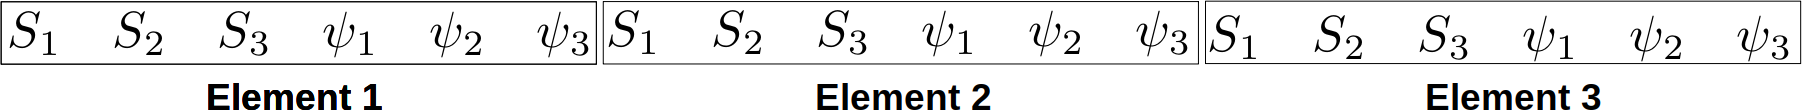
\includegraphics[width=0.9\textwidth]{images/blockStructure.png}
	\label{fig:blockStructureScheme}
	\caption{Schematic representation of the components in the solution vector for the 1st order ODE and compact DAE formulations on three elements}
\end{figure}

This block structure is also applied to the Jacobian matrices, such that they can be directly used in the Newton iteration. Setting up the matrix and the block matrix transformations in \autoref{ssec:iterative_solver_Jacobian} required thus nasty index operations.

\subsection{Memory requirements}
When the simulation will be scaled up to larger domain, memory requirements have to be taken into account. The most problematic term here will be the full matrix $\pdv{f}{S}$, whose size increases quadratically with the number of fault nodes. For example, a domain with 10 000 fault elements and 3 nodes per fault requires, if all components are stored with double precision, 57.6GB memory just for the Jacobian matrix. Typically, such large simulations will be run on multiple cores once the code is parallelized, and the matrix is stored on multiple processors. The communication overhead to solve the Newton update will seriously hamper the performance, since there is no apparent pattern in $\pdv{f}{S}$ that could be efficiently used with parallel iterative solvers. The 1st order ODE with an explicit time integration is the only method that does not require to set up the dense matrix $\pdv{f}{S}$ and is not affected by these considerations. 

